
\documentclass [PhD] {uclathes}

% Packages
\usepackage{xspace}
\usepackage{amsmath}
\usepackage{graphicx}
\usepackage{hyperref}
\hypersetup{
  colorlinks=true,
  citecolor=blue,
  linkcolor=blue,
  urlcolor=magenta
}
\usepackage{topcapt}
\usepackage{multirow}

% Words
\newcommand {\etal}{\mbox{et al.}\xspace}
\newcommand {\ie}{\mbox{i.e.}\xspace}
\newcommand {\eg}{\mbox{e.g.}\xspace}
\newcommand {\etc}{\mbox{etc.}\xspace}
\newcommand {\vs}{\mbox{vs.}\xspace}

% Particles
\newcommand{\Pp}{\ensuremath{\mathrm{p}}}
\newcommand{\PZ}{\ensuremath{\mathrm{Z}}}
\newcommand{\Pgm}{\ensuremath{\mathrm{\mu}}}

% Units
\newcommand{\unit}[1]{\ensuremath{\text{\,#1}}\xspace}
%% Energy
\newcommand{\keV}{\ensuremath{\,\text{ke\hspace{-.08em}V}}\xspace}
\newcommand{\keVns}{\ensuremath{\text{ke\hspace{-.08em}V}}\xspace}
\newcommand{\GeV}{\ensuremath{\,\text{Ge\hspace{-.08em}V}}\xspace}
\newcommand{\GeVns}{\ensuremath{\text{Ge\hspace{-.08em}V}}\xspace}
\newcommand{\MeV}{\ensuremath{\,\text{Me\hspace{-.08em}V}}\xspace}
\newcommand{\MeVns}{\ensuremath{\text{Me\hspace{-.08em}V}}\xspace}
\newcommand{\TeV}{\ensuremath{\,\text{Te\hspace{-.08em}V}}\xspace}
\newcommand{\TeVns}{\ensuremath{\text{Te\hspace{-.08em}V}}\xspace}
%% Length
\newcommand{\cm}{\ensuremath{\,\text{cm}}\xspace}
\newcommand{\mm}{\ensuremath{\,\text{mm}}\xspace}
%% Time
\newcommand{\mus}{\ensuremath{\,\mu\text{s}}\xspace}
%% Other
\newcommand{\fbinv} {\mbox{\ensuremath{\,\text{fb}^{-1}}}\xspace}
\newcommand{\percms}{\ensuremath{\,\text{cm}^{-2}\,\text{s}^{-1}}\xspace}
\newcommand{\muA}{\ensuremath{\,\mu}A\xspace}

% Names
\newcommand{\GEANTfour}{{\textsc{Geant4}}\xspace}
\newcommand {\Lone}{Level-1\xspace}

% Symbols
\newcommand{\pt}{\ensuremath{p_{\mathrm{T}}}\xspace}

% Combo symbols
\newcommand{\pp}{\Pp\Pp\xspace}
\newcommand{\ZMM}{\PZ$\to$\Pgm\Pgm\xspace}
\newcommand{\chem}[2]{$^{#1}$#2}

% Constants
\newcommand{\reflumi}{\ensuremath{10^{34}}\percms}

% Formatting
\newcommand{\posstyle}[1]{#1}

% CMS formatting wants Fig. in the middle of a sentence,
% and Eq. and Eqs. always, but I don't
%\newcommand{\Eq}{Eq.}
%\newcommand{\Eqs}{Eqs.}
%\newcommand{\Fig}{Figure}
%\newcommand{\FigDot}{Fig.}
%\newcommand{\Figs}{Figures}
%\newcommand{\FigsDot}{Figs.}
%\newcommand{\Sec}{Section}
%\newcommand{\Secs}{Sections}
%\newcommand{\Tab}{Table}
%\newcommand{\Tabs}{Tables}
\newcommand{\Eq}{Equation}
\newcommand{\Eqs}{Equations}
\newcommand{\Fig}{Figure}
\newcommand{\FigDot}{Figure}
\newcommand{\Figs}{Figures}
\newcommand{\FigsDot}{Figures}
\newcommand{\Sec}{Section}
\newcommand{\Secs}{Sections}
\newcommand{\Tab}{Table}
\newcommand{\Tabs}{Tables}

% Math
\newcommand{\dd}[1]{\ensuremath{\mathop{}\!\mathrm{d}#1}}
\newcommand{\vc}[1]{\ensuremath{\mathbf{#1}}}

\newlength\dummyFigWidth
\setlength\dummyFigWidth{0.85\textwidth}
\newlength\halfFigWidth
\setlength\halfFigWidth{0.6\dummyFigWidth}
\newlength\twoThirdsFigWidth
\setlength\twoThirdsFigWidth{0.77\dummyFigWidth}
\newlength\fullFigWidth
\setlength\fullFigWidth{1.17\dummyFigWidth}

\clubpenalty=9999
\widowpenalty=9999
\newcommand{\ExtraClearPage}{\clearpage}
                         % personal LaTeX macros

%%%%%%%%%%%%%%%%%%%%%%%%%%%%%%%%%%%%%%%%%%%%%%%%%%%%%%%%%%%%%%%%%%%%%%
%
% Usually things live in separate flies.
%
% \input {prelim}                           % preliminary page info

%%%%%%%%%%%%%%%%%%%%%%%%%%%%%%%%%%%%%%%%%%%%%%%%%%%%%%%%%%%%%%%%%%%%%%%%
%                                                                      %
%                          PRELIMINARY PAGES                           %
%                                                                      %
%%%%%%%%%%%%%%%%%%%%%%%%%%%%%%%%%%%%%%%%%%%%%%%%%%%%%%%%%%%%%%%%%%%%%%%%

\title          {My Very First PhD Thesis}
\author         {Abhigyan (Riju) Dasgupta}
\department     {Physics}
% Note:  degreeyear should be optional, but as of  5-Feb-96
% it seems required or you get a year of ``2''.   -johnh
\degreeyear     {2019}

%%%%%%%%%%%%%%%%%%%%%%%%%%%%%%%%%%%%%%%%%%%%%%%%%%%%%%%%%%%%%%%%%%%%%%%%

\chair          {Robert Cousins}
\member         {Zvi Bern}
\member         {Jay Hauser}
\member         {David Saltzberg}

%%%%%%%%%%%%%%%%%%%%%%%%%%%%%%%%%%%%%%%%%%%%%%%%%%%%%%%%%%%%%%%%%%%%%%%%

\dedication     {\textsl{Dedication}}

%%%%%%%%%%%%%%%%%%%%%%%%%%%%%%%%%%%%%%%%%%%%%%%%%%%%%%%%%%%%%%%%%%%%%%%%

\acknowledgments {(Acknowledgments omitted for brevity.)}

%%%%%%%%%%%%%%%%%%%%%%%%%%%%%%%%%%%%%%%%%%%%%%%%%%%%%%%%%%%%%%%%%%%%%%%%

\vitaitem   {2009--2013}
            {Undergraduate Research Assistant, CONCEPT Laboratory, UC Berkeley.}
\vitaitem   {2013}
            {B.A.~(Physics) and B.A.~(Mathematics), UC Berkeley.}
\vitaitem   {2013--2015}
            {Teaching Assistant, Physics Department, UCLA.}
\vitaitem   {2014}
            {M.S.~(Physics), UCLA.}
\vitaitem   {2015--present}
            {Graduate Student Researcher, Physics Department, UCLA.
             Based full time at CERN on the Franco-Swiss border.}

%%%%%%%%%%%%%%%%%%%%%%%%%%%%%%%%%%%%%%%%%%%%%%%%%%%%%%%%%%%%%%%%%%%%%%%%

\publication    {\textsl{Title} Info}

%%%%%%%%%%%%%%%%%%%%%%%%%%%%%%%%%%%%%%%%%%%%%%%%%%%%%%%%%%%%%%%%%%%%%%%%

\abstract       {(Abstract omitted for brevity)}

%%%%%%%%%%%%%%%%%%%%%%%%%%%%%%%%%%%%%%%%%%%%%%%%%%%%%%%%%%%%%%%%%%%%%%%%

\begin {document}
\phantomsection
\makeintropages

%%%%%%%%%%%%%%%%%%%%%%%%%%%%%%%%%%%%%%%%%%%%%%%%%%%%%%%%%%%%%%%%%%%%%%

\chapter{Introduction}
I am an introduction.

\chapter{Theory}
The Standard Model is awesome.

\chapter{The CMS Detector at the CERN LHC}
\label{chap:cms}
\PretentiousQuote{The expectations of life depend upon diligence; the mechanic that would perfect his work must first sharpen his tools.}{Confucius}{Analects of Confucius}

The Compact Muon Solenoid (CMS) detector is a general-purpose detector for studying the physics of fundamental particles produced by proton-proton (\pp) and heavy ion collisions at the Large Hadron Collider (LHC) at CERN.
Two beams of protons circle the 27.6\unit{km} circumference of the LHC in opposite directions and collide at various locations along it; one of these locations is the CMS detector.

\section{The CERN LHC}
The LHC is a two-ring circular hadron collider designed to collide protons at a center-of-mass energy of $\sqrt{s} = 14\TeV$ and at a design instantaneous luminosity of $\lumi = 10^{34} \cm^{-2} \unit{s}^{-1}$ \cite{Evans:2008zzb}.
Run 2 of the LHC began in 2015 with its superconducting dipole magnets operating such that the corresponding center-of-mass energy is $\sqrt{s} = 13\TeV$ \cite{Todesco:2017tcj}.

\subsection{Accelerator Complex, Proton Injection Chain, and Bunch Structure}
\Fig~\ref{cms:lhc} is a diagram of the CERN accelerator complex.
The LHC tunnel has eight arcs and eight straight sections.
Each straight section can serve as a location for experiments, but only four are used as such.
Beam crossings occur at four of these points: the locations of the four largest experiments at the LHC.
The two high-luminosity, general-purpose experiments, CMS and ATLAS, are located at Point~5 and Point~1, respectively.
The two lower luminosity, more special purpose experiments, ALICE and LHCb, are located at Point~2 and Point~8, respectively.
Yellow dots indicate these four experiments in \Fig~\ref{cms:lhc}, each with their own large detectors in underground caverns receiving collisions from the LHC.

\begin{figure}[p]
  \centering
  \includegraphics[width=0.8\textwidth]{figures/cms/LHCAcceleratorComplex.pdf}
  \caption[Overview of the CERN accelerator complex.]{Overview of the CERN accelerator complex, reproduced from Reference~\cite{Mobs:2636343}.}
  \label{cms:lhc}
\end{figure}

\begin{figure}[p]
  \centering
  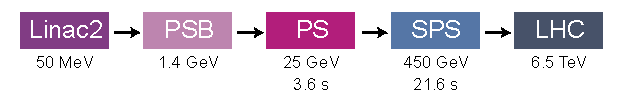
\includegraphics[width=0.8\textwidth]{figures/cms/InjectionChain.pdf}
  \caption[Summary of the injection chain of the LHC.]{Summary of the injection chain of the LHC, including the proton beam energy, which increases at each step, and (for the PS and SPS) the synchrotron cycle time. Multiple cycles of the PS and SPS are required to fill the LHC.}
  \label{cms:injectionchain}
\end{figure}

\Fig~\ref{cms:injectionchain} is a diagram summarizing the injection chain by which protons are accelerated in the LHC.
Protons begin at Linac2, a linear accelerator, and are subsequently injected into the Proton Synchrotron Booster (PSB), the Proton Synchrotron (PS), the Super Proton Synchrotron (SPS), and finally the LHC.
Filling the LHC requires 12 cycles of the SPS and 3--4 cycles of the PS, yielding a total LHC filling time of approximately 4 minutes per beam.

Proton beams at the LHC are not continuous streams of protons, but rather organized into high-intensity bunches spaced 25\unit{ns} apart, corresponding to a crossing frequency of 40\unit{MHz}.
The LHC has 3564 bunch places, of which up to 2808 are filled with protons in colliding bunches.
Consecutive bunches of protons occur in trains of filled bunches separated by gaps.
Proton-proton collisions occur when bunches of protons cross, called bunch crossings.
\Fig~\ref{cms:lhcbunchpattern} is a diagram showing the 3564 bunch places, each represented by a square, and the pattern of filled bunches, represented by squares filled in blue.

\begin{figure}[tpb]
  \centering
  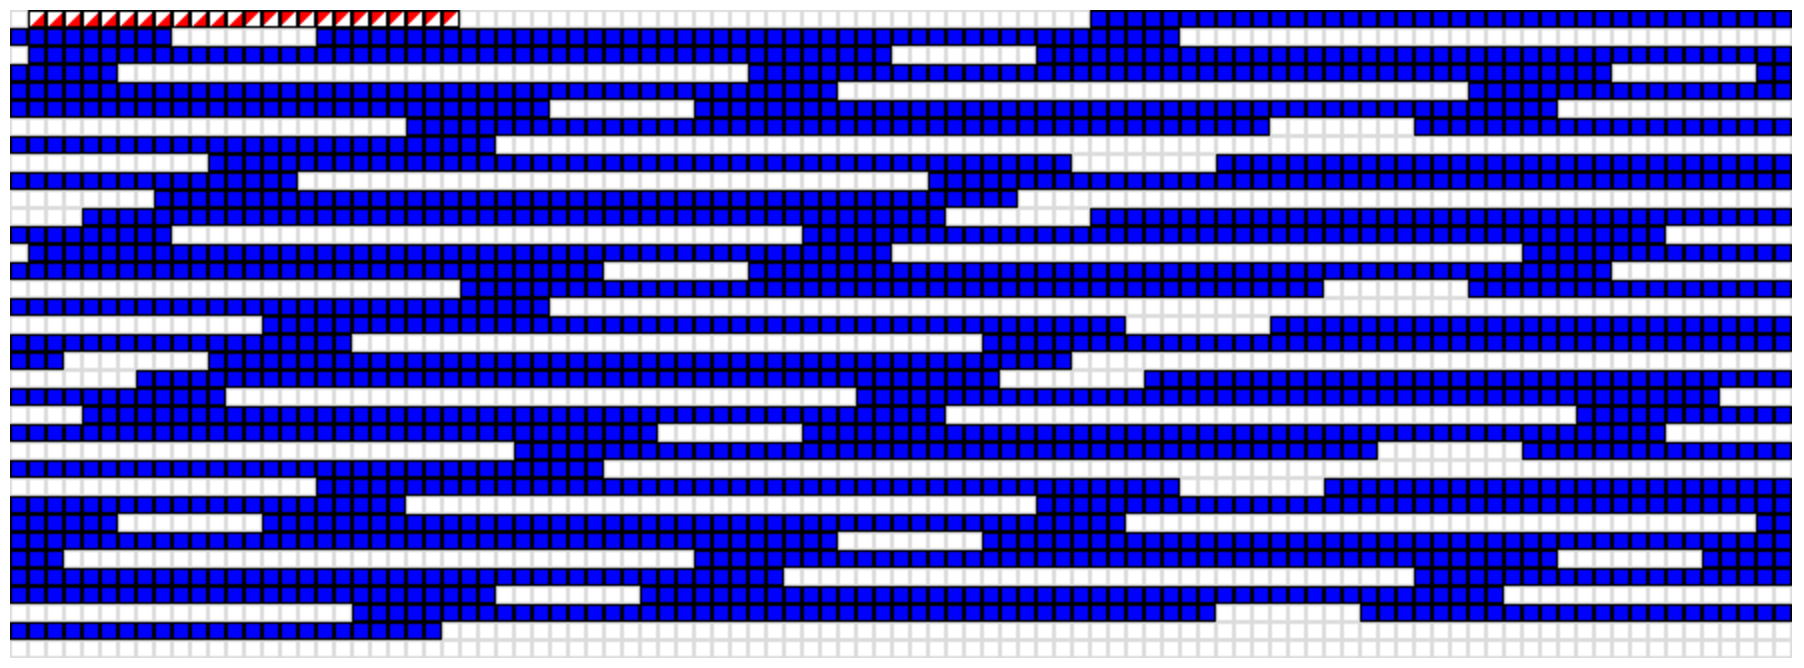
\includegraphics[width=0.8\textwidth]{figures/cms/Fill5423BunchPattern.png}
  \caption[Diagram of the bunch places of an LHC proton beam showing filled and empty places.]{Diagram of the bunch places of an LHC proton beam, showing filled bunches (blue) and empty places (gray). The grid is $99 \times 36 = 3564$ squares, \ie they wrap around. Reproduced from Reference~\cite{CMSWBM:Fill5423} for Fill 5423 of the LHC in October 2016.}
  \label{cms:lhcbunchpattern}
\end{figure}

\subsection{RF Cavities and Steering Magnets}
Protons are accelerated from the 450\GeV of the SPS to the 6.5\TeV of the LHC by a system of eight radio frequency (RF) cavities.
These RF cavities oscillate at 400\unit{MHz} at a maximum amplitude of 2\unit{MV}, for a total of 16\unit{MV} per beam, increasing the proton energy by about 0.5\MeV per revolution.

The phase of the RF waveform is carefully modulated to create and maintain bunches of protons, and to accelerate them to and maintain them at the desired energy.
The 3564 bunch places of the LHC are separated by 25\unit{ns}, meaning a bunch place passes through a particular RF cavity at a frequency of 40\unit{MHz}.
The RF cavity frequency is ten times that: 400\unit{MHz}.
This divides a bunch place into ten RF buckets, which are individual regions of space in which a bunch of protons can be confined, the shape and size of which are determined by the RF voltage amplitude and the number of bunch places.
When coasting (at collision energy), a (hypothetical) particle with energy such that the RF frequency is exactly an integer multiple of the orbit frequency, synchronized such that the particle passes through the RF cavity at exactly a time of zero voltage within the RF waveform is called a synchronous particle.
Particles with higher or lower energy or arriving early or late with respect to the synchronous particle will experience a non-zero voltage and therefore experience a restoring force.
These particles oscillate longitudinally around the synchronous particle.
The size of an RF bucket is given as an area in energy-time phase space, defined with respect to a synchronous particle: it is parametrized by the maximum energy deviation of a particle within the bunch from that of the synchronous particle (in \unit{eV}) and the maximum deviation in arrival time of a particle within the bunch from that of the synchronous particle (in seconds).
A proton bunch occupies a single RF bucket and is depicted by an ellipse within the bucket in energy-time phase space, representing the trajectory of particles within the bunch.
An LHC proton bunch has a 4$\sigma$ bunch length of 1.06\unit{ns} at collision energy.
\Fig~\ref{cms:rfbucket} depicts an RF bucket, football-shaped in energy-time phase space, as well as the ellipse contained within it that represents the proton bunch. The area of the bunch in this diagram is called the longitudinal emittance, with units of $\text{eV}\cdot\text{s}$.

\begin{figure}[p]
  \centering
  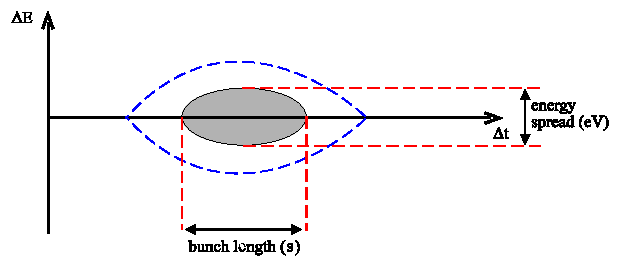
\includegraphics[width=0.8\textwidth]{figures/cms/RFBucket.pdf}
  \caption[Phase space diagram of an RF bucket and the elliptical boundary of a proton bunch within the bucket.]{Phase space diagram of an RF bucket and the elliptical boundary of a proton bunch within the bucket, reproduced from Reference~\cite{Baird:1017689} with minor typographical corrections.}
  \label{cms:rfbucket}
\end{figure}

Beams of particles in the LHC are steered by a network of 1232 superconducting dipole magnets, interspersed with quadrupole magnets for focusing.
The superconducting wire windings in these magnets are made of niobium-titanium, cooled by liquid helium to their operating temperature of 1.9\unit{K}, and producing a magnetic field of 8.33\unit{T}.
\Fig~\ref{cms:dipole} is a diagram of the cross section of an LHC dipole magnet as well as a visualization of the magnetic field lines within the beam pipe.

\begin{figure}[p]
  \centering
  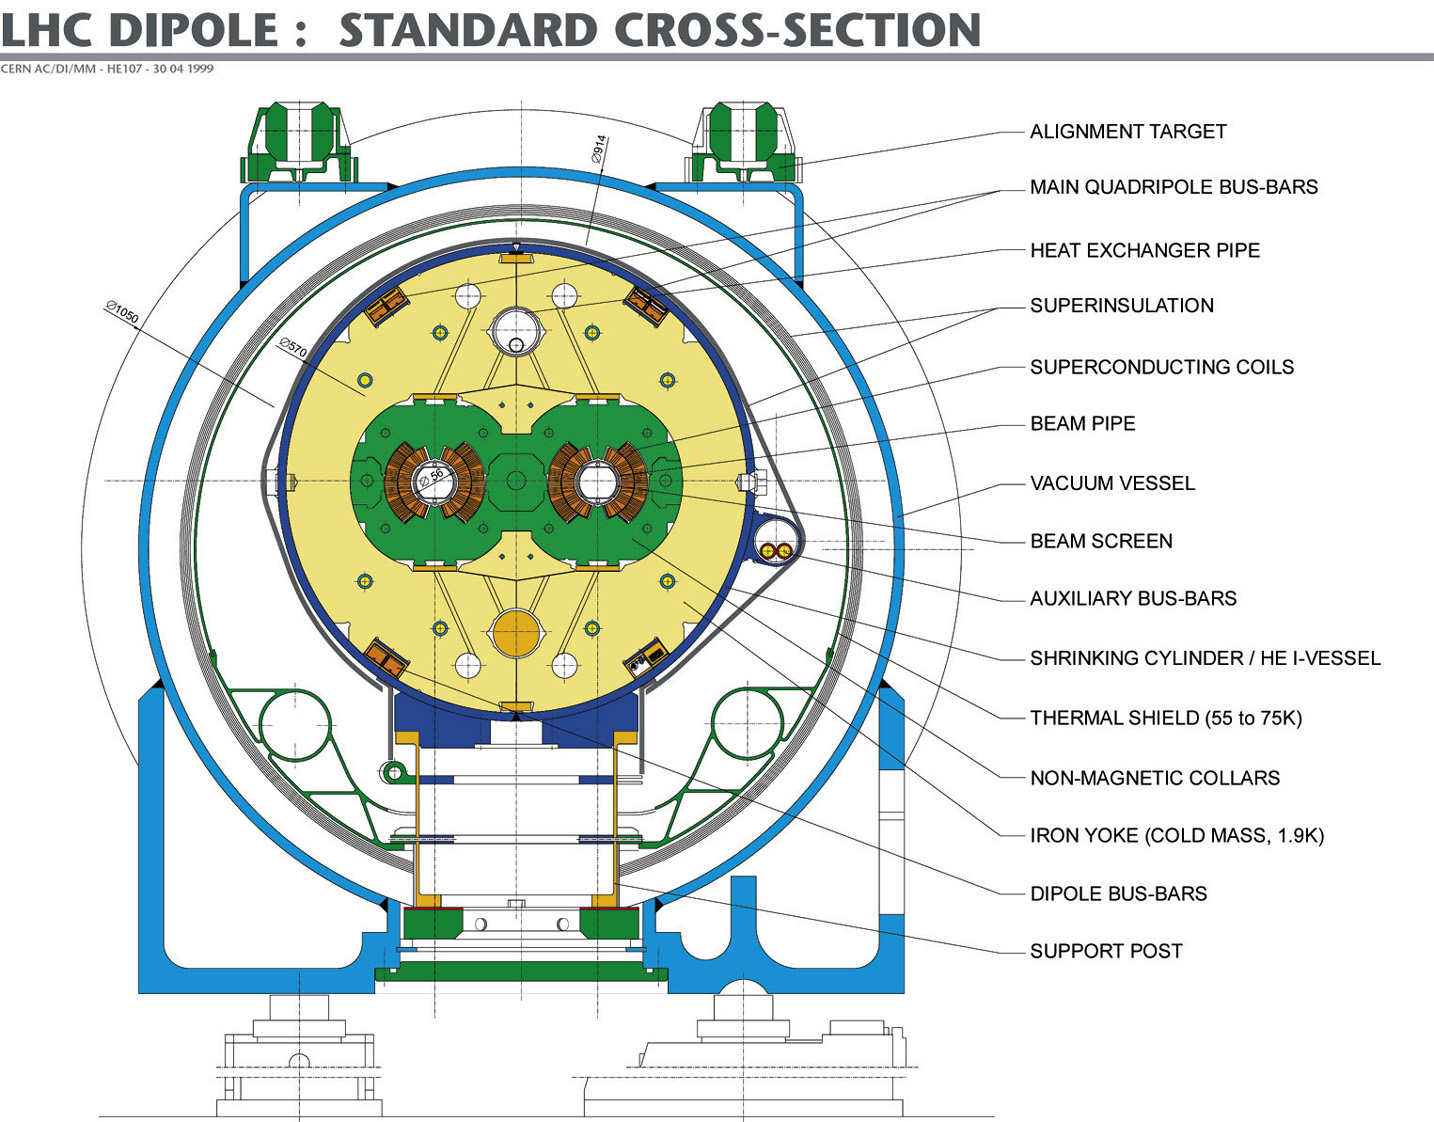
\includegraphics[width=0.55\textwidth]{figures/cms/DipoleCrossSection.jpeg}
  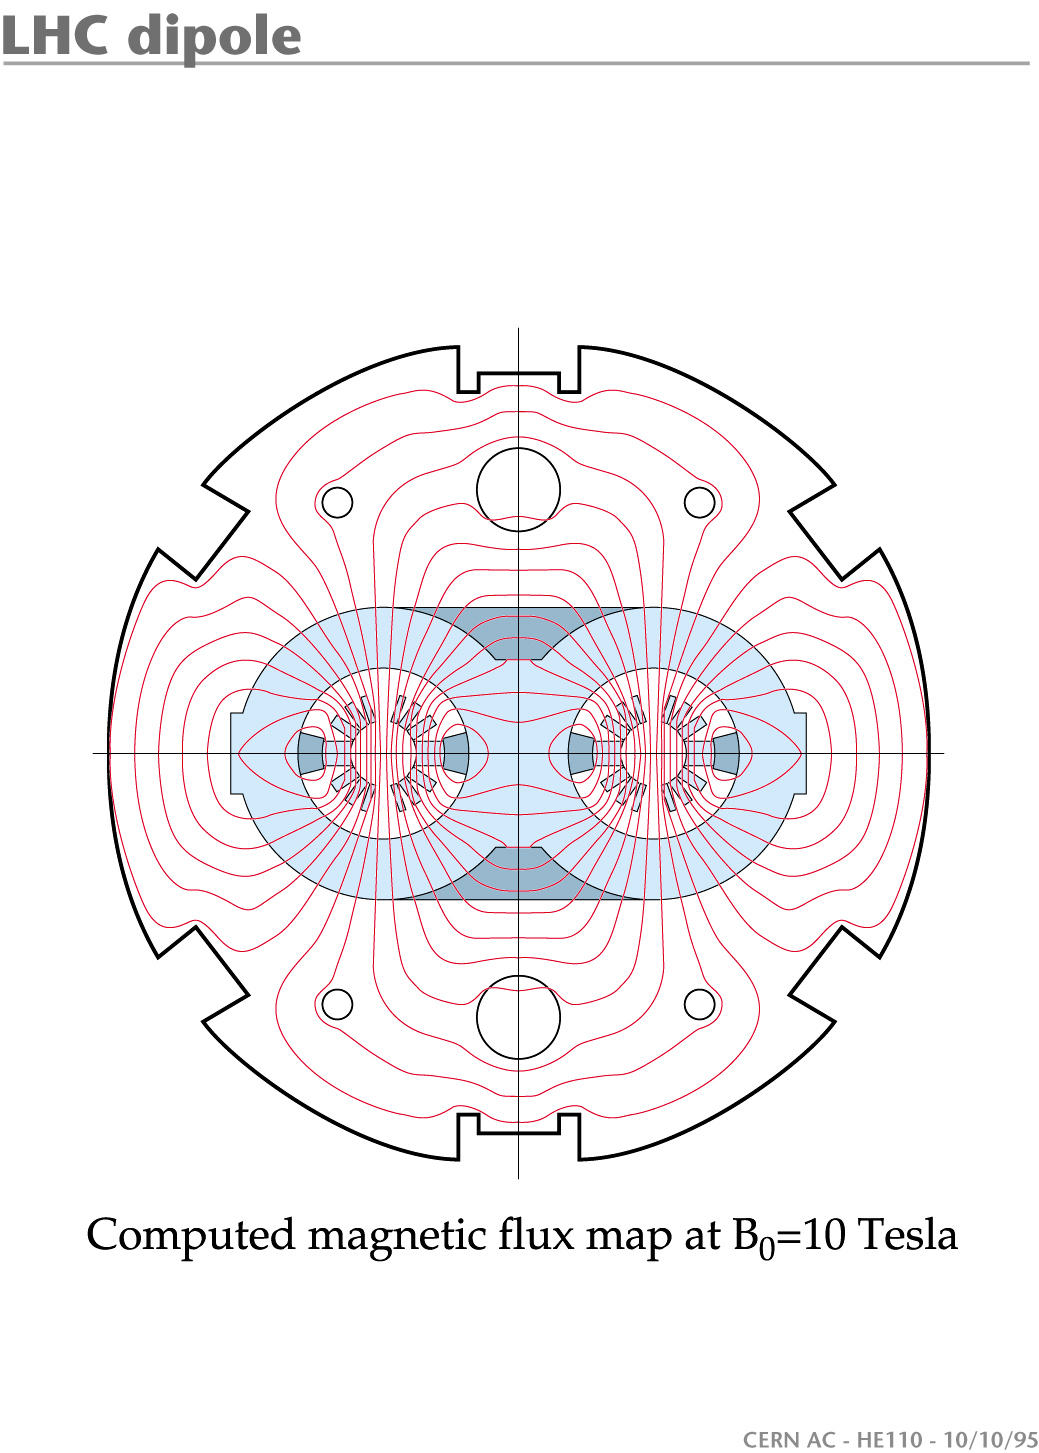
\includegraphics[width=0.35\textwidth]{figures/cms/FieldLines.jpg}
  \caption[Diagram of cross section of an LHC steering dipole magnet and depiction of the magnetic field lines in the magnets.]{(left) Diagram of cross section of an LHC steering dipole magnet, reproduced from Reference~\cite{Team:40524}, showing the two beam pipes and the windings. (right) Depiction of the magnetic field lines in the magnets, reproduced from Reference~\cite{Jean-Luc:841503}, showing them to point in the vertical direction within the beam pipe, as is required to circulate particles along the surface of the earth.}
  \label{cms:dipole}
\end{figure}

\subsection{Instantaneous and Integrated Luminosity}
The number of events per second generated by the LHC for a process of cross section $\sigma$ is
\begin{equation}
  \frac{\dd N}{\dd t} = \lumi \sigma
  \label{cms:nEvents}
\end{equation}
where $\lumi$ is the instantaneous luminosity, and depends only on machine parameters:
\begin{equation}
  \lumi = \frac{N_p^2 N_b f \gamma}{4 \pi \epsilon \beta^*} R 
  \label{cms:instlumi}
\end{equation}
where $R$ is a geometrical factor accounting for the beam crossing angle,
\begin{equation}
  \frac{1}{R} = \sqrt{1 + \left(\frac{\theta\sigma_z}{2\sigma^*}\right)^2}
  \label{cms:geo}
\end{equation}
The design LHC beam parameters in \Eqs~\ref{cms:instlumi}--\ref{cms:geo} are defined and summarized in \Tab~\ref{cms:beam} \cite{Baird:1017689, Bruning:782076}.
This yields a peak instantaneous luminosity of $\lumi = 10^{34} \,  \mathrm{cm}^{-1} \, \mathrm{s}^{-1}$.

\begin{table}
  \centering
  \begin{tabular}{lll}
    \hline
    Symbol     & Name                                                          & Value                 \\ \hline
    $N_p$      & protons per bunch                                             & $1.15 \times 10^{11}$ \\
    $N_b$      & bunches per beam                                              & 2808                  \\
    $f$        & revolution frequency (1/24.95\unit{ns}/3564)                  & 11.25\unit{kHz}       \\
    $\gamma$   & relativistic Lorentz factor for protons ($E_p/m_p$)           & 7461                  \\
    $\epsilon$ & normalized transverse beam emittance                          & 3.75\mum              \\
    $\beta^*$  & optical $\beta$ function (amplitude of betatron oscillations) & 55\unit{cm}           \\
    $\theta$   & beam crossing angle                                           & 285 $\mu\text{rad}$   \\
    $\sigma_z$ & longitudinal RMS bunch length                                 & 7.55\unit{cm}         \\
    $\sigma^*$ & transverse RMS beam size                                      & 16.7\mum              \\
    & & \\ \hline
  \end{tabular}
  \caption[LHC nominal design beam parameters.]{LHC nominal design beam parameters, reproduced from Reference~\cite{Bruning:782076}.}
  \label{cms:beam}
\end{table}

Proton collisions lead to a natural decrease in luminosity over time, with a luminosity lifetime of 15--25 hours.
The integral of the instantaneous luminosity over time is called the integrated luminosity, $\intlumi$.
The total number of events generated by the LHC for a process of cross section $\sigma$ is then given by the integrated luminosity times the cross section, so that
\begin{align}
  N = \sigma \int{\lumi\,\dd t} = \sigma \intlumi
  \label{cms:intlumi}
\end{align}
Since the \pp interaction cross section is a constant, the total integrated luminosity delivered to (and recorded by) an experiment is therefore also a measure of the number of events and hence the amount of data recorded by the experiment.
For convenience with handling large exponents, the integrated luminosity is given in inverse femtobarns: $1\unit{fb} = 10^{-39}\unit{cm}^2$.
\Fig~\ref{cms:totallumi} is a plot of the total \pp integrated luminosity over time, by year and calendar month, for the entirety of Run~1 and Run~2.
This thesis presents two analyses using data taken by the CMS experiment in 2016: a search for displaced dimuons using the full 2016 integrated luminosity of 35.9\fbinv, and a study of neutron-induced background in muon chambers using one era of 2016 data taking, corresponding to 8.73\fbinv.

\begin{figure}[tpb]
  \centering
  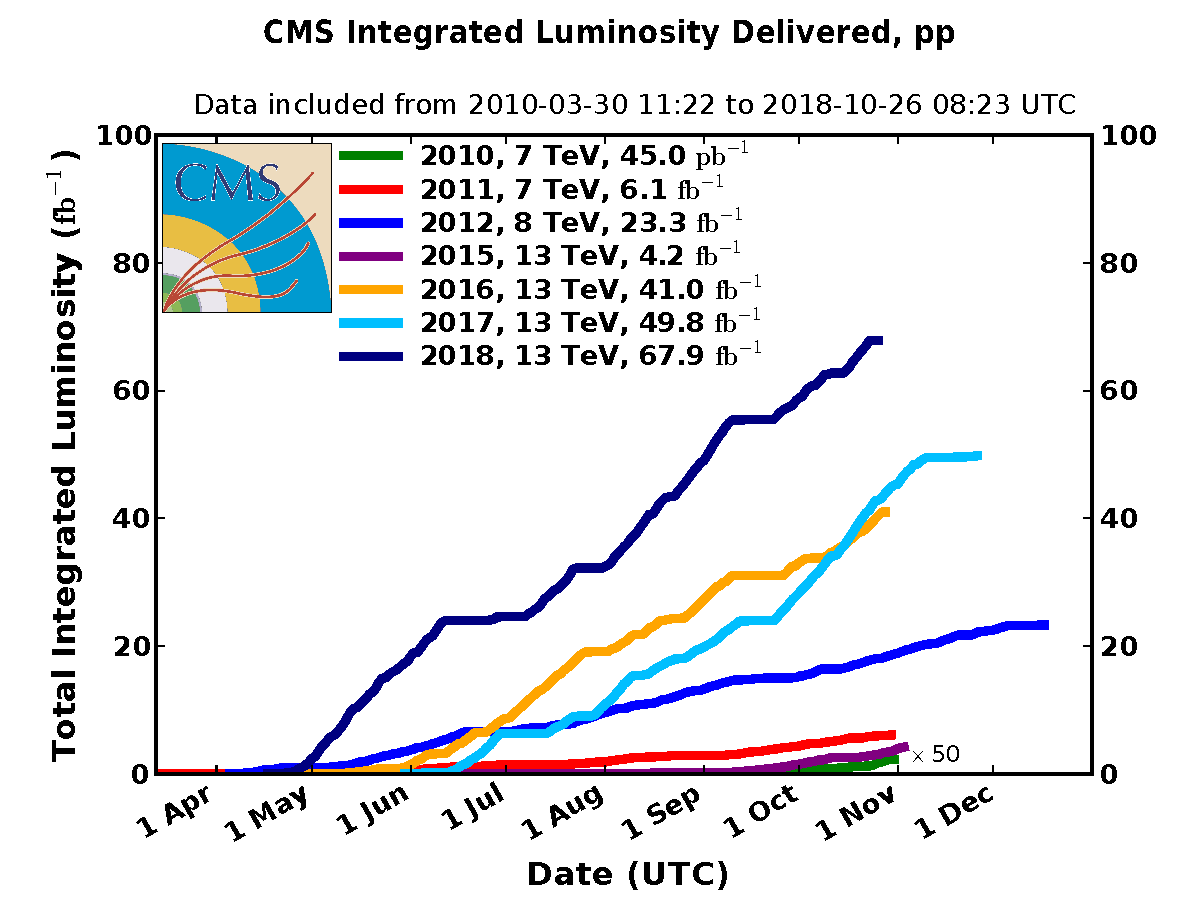
\includegraphics[width=0.8\textwidth]{figures/cms/CMSIntLumi.pdf}
  \caption[Total \pp integrated luminosity recorded by CMS during Run~1 and Run~2 by year and month.]{Total \pp integrated luminosity recorded by CMS during Run~1 and Run~2 by year and month, reproduced from Reference~\cite{LumiTwiki}.}
  \label{cms:totallumi}
\end{figure}

\section{The CMS Detector}
\subsection{Introduction}
\label{cms:intro}
CMS is located at Point~5 of the LHC in the commune of Cessy in eastern France, at the level of the LHC beam line, 100\unit{m} underground.
Its overall shape is a cylinder 15\unit{m} in diameter and 21.6\unit{m} in length, weighing 14,000 tons.
It is named for three of its distinguishing features: its \textbf{c}ompactness, its \textbf{m}uon system, and its \textbf{s}olenoid magnet.
A large magnetic field with high bending power is required to precisely measure the momentum of high-energy charged particles.
This informs a choice of superconducting technology, and so a superconducting solenoid magnet sits at the heart of the cylindrically symmetric CMS detector, producing a continuous magnetic field of 3.8\unit{T}.
CMS is quite compact for all the detector material it contains, especially compared to ATLAS.
Notably, the bulk of the CMS hadronic calorimeter is completely contained the solenoid magnet, with important consequences for its design.
The muon system, on the other hand, is outside the solenoid.
Muons are one of the five general categories of particles directly detected by CMS, and unique among them in that they typically neither stop nor decay within the boundaries of the detector.
They are less subject to energy losses when passing through detector material than electrons and so provide a powerful lens with which to study high-energy processes in the presence of high background.
The outermost bulk of CMS is thus a dedicated system for identifying and measuring muons, consisting of three kinds of gas ionization detectors \cite{Chatrchyan:2008zzk}.

The CMS detector is structured like an onion, in layers, consisting of the following basic subsystems, ordered from innermost to outermost:
\begin{itemize}
  \item silicon tracker
  \item electromagnetic calorimeter
  \item hadronic calorimeter
  \item superconducting solenoid magnet
  \item muon system
\end{itemize}

\Fig~\ref{cms:interactive} is a diagram of a slice of the CMS detector illustrating these layers.
\begin{figure}[tpb]
  \centering
  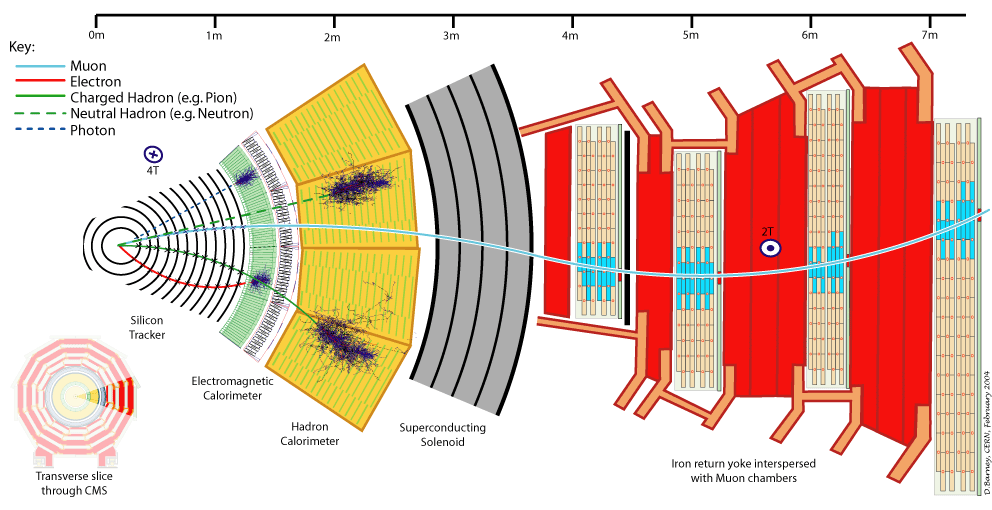
\includegraphics[width=\textwidth]{figures/cms/CMSSlice.png}
  \caption[Transverse slice of the CMS detector illustrating the basic structure of CMS and the shapes of the tracks and energy deposits formed by the five general categories of particles directly detected by CMS.]{Transverse slice of the CMS detector, reproduced from Reference~\cite{Davis:2205172}, illustrating the basic structure of CMS and the shapes of the tracks and energy deposits formed by the five general categories of particles directly detected by CMS by one or more of its subsystems.}
  \label{cms:interactive}
\end{figure}
It also shows the detector signatures of the general categories of particles directly detected by CMS:
\begin{itemize}
  \item electrons
  \item photons
  \item charged hadrons
  \item neutral hadrons
  \item muons
\end{itemize}
The charged particles---electrons, muons, and charged hadrons---are detected as they form curved, helical tracks in the silicon tracker (and in the case of muons, in the muon system as well).
Electrons, charged hadrons, and the neutral particles---photons and neutral hadrons---leave energy deposits in the electromagnetic and hadronic calorimeters.

\subsection{Coordinate System}
The origin of the coordinate system used by CMS is the nominal \pp collision point.
The $y$-axis points upwards, the $x$-axis points radially inwards towards the center of the LHC, approximately south, and thus the $z$-axis points approximately west.
The azimuthal angle $\phi$ about the $z$-axis is measured from the $x$-axis and the radial coordinate in the $xy$-plane is denoted $r$.
The polar angle measured from the $z$-axis is denoted $\theta$.
However, a more conventional coordinate used in hadron collider physics is the pseudorapidity $\eta$, defined as
\begin{equation}
  \eta = -\ln\tan\left(\frac{\theta}{2}\right)
  \label{eq:eta}
\end{equation}
For a particle of three-momentum $\vc{p}$ with $z$-component $p_z$, pseudorapidity can be written
\begin{equation}
  \eta = \frac12\ln\left(\frac{|\vc{p}|+p_z}{|\vc{p}|-p_z}\right)
  \label{eq:eta_p}
\end{equation}
This form elucidates its relationship to rapidity (along the $z$-axis),
\begin{equation}
  y = \frac12\ln\left(\frac{E+p_z}{E-p_z}\right),
  \label{eq:rap}
\end{equation}
which is a quantity Lorentz invariant under boosts in the $z$-direction \cite{Hama:1981}.
The pseudorapidity has the advantage that it converges to rapidity (along the $z$-axis) in the high-velocity, low-mass limit (as $|\vc{p}|\to E$), and is only dependent on the polar angle $\theta$ and not on the energy of the particle.
\Fig~\ref{cms:quadrant} is a schematic diagram of one quadrant of CMS, showing the placement of the components of CMS within the coordinate system.
\begin{figure}[tpb]
  \centering
  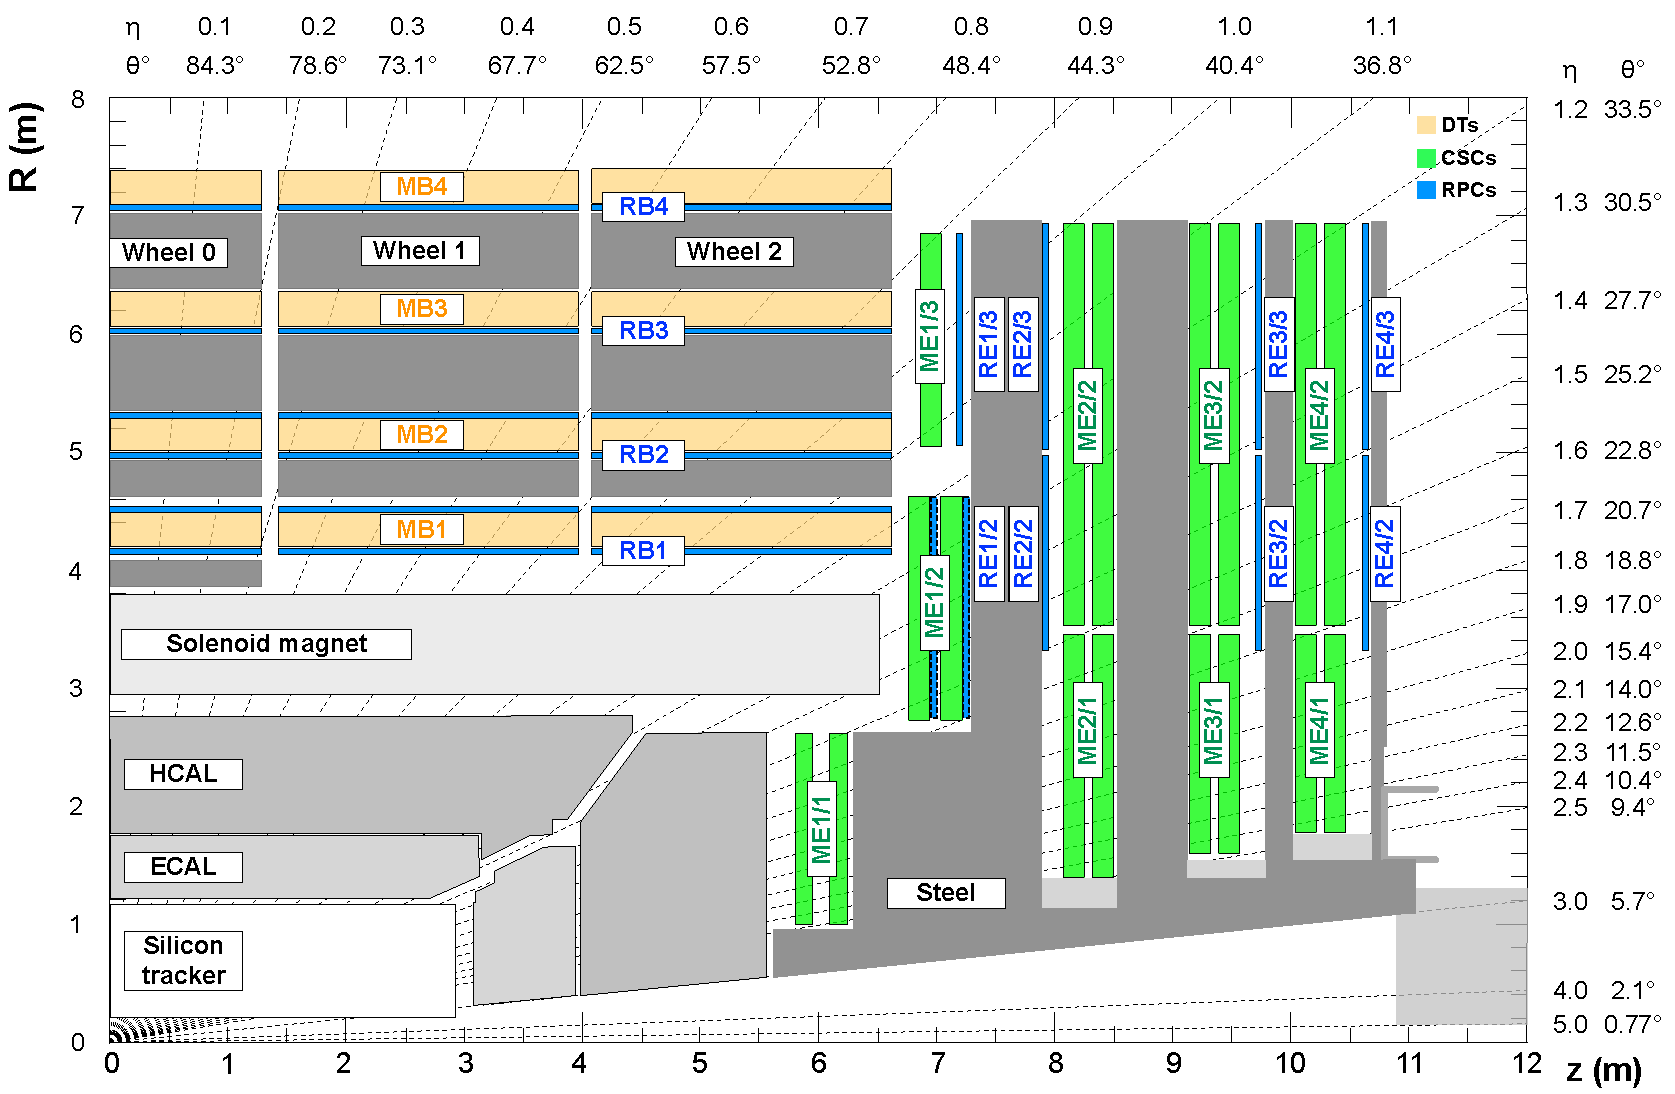
\includegraphics[width=\textwidth]{figures/cms/CMSGeometry.pdf}
  \caption[Schematic diagram of one quadrant of CMS in $r$-$z$.]{Schematic diagram of one quadrant of CMS in $r$-$z$, reproduced from Reference~\cite{Sirunyan:2018fpa}, illustrating the position of all the subsystems with respect to the coordinate system, in both the barrel and the endcap.}
  \label{cms:quadrant}
\end{figure}

The diagram illustrates that $\eta = 0$ points upwards, while $\eta \to \infty$ points along the $z$-axis.
For this reason the ``forward'' regions close to the beam line (which are also less instrumented) are referred to as ``high $\eta$.''
The diagram also illustrates two distinct loci within the CMS detector: the barrel, which covers approximately (depending on subsystem) the region $|\eta| < 1.2$, and the endcap, which covers approximately (depending on subsystem) the region $1.2 < |\eta| < 3$.

\subsection{Silicon Tracker}
The inner tracking system of CMS must provide precise measurements of charged particle trajectories and reconstructions of secondary vertices of (on average) a thousand particles every 25\unit{ns} bunch crossing, exposed to the full flux of the radiation of the LHC.
These requirements on precision, speed, and radiation hardness inform a choice of silicon detector technology.
The ionization induced by an energetic charged particle passing through produces electron-hole pairs, which are measured as current in the presence of an applied voltage.

The CMS tracker consists of two silicon detector technologies: pixels and strips.
The innermost component of the tracker, closest to the collision point, is the pixel detector, consisting of three barrel layers and two endcap disks on each side of the barrel.
The 66 million silicon pixel sensors are $n$-on-$n$ devices, measuring $100 \mum \times 150 \mum$, giving a spatial resolution of 15--20\mum.
Just outside the pixel detector is the strip detector, consisting of ten barrel layers and twelve endcap disks on each side of the barrel.
The 9.6 million silicon strip sensors are $p$-on-$n$ type microstrip sensors, manufactured on 6\unit{in} wafers, varying in width from 80--180\mum.
The CMS tracker measures transverse momentum ($\pT$) to a resolution of 1\% for 100\GeV particles.
Containing altogether 205~$\text{m}^2$ of silicon sensors with 75 million individual channels, the CMS tracker is the largest silicon detector in the world \cite{Chatrchyan:2008zzk, CERN-LHCC-98-006, HARTMANN201225}.


\subsection{Electromagnetic Calorimeter}
The electromagnetic calorimeter (ECAL) was designed to achieve the excellent energy resolution critical for observing the decay of the SM Higgs boson to two photons: $H \to \gamma\gamma$.
The ECAL is a homogeneous calorimeter consisting of about 76,000 scintillating lead tungstate (PbWO$_4$) crystals, a material chosen for its high density and short radiation length.
Electrons or photons passing through the detector material result in a cascade of electromagnetic interactions, producing a shower of particles culminating in a release of energy proportional to the energy of the incident particle.
The corresponding photons are then measured by photodetectors installed on each crystal \cite{Chatrchyan:2008zzk, CERN-LHCC-97-033, Fabjan:692252}.

\subsection{Hadronic Calorimeter}
The hadronic calorimeter (HCAL) is a sampling calorimeter: it consists of repeating, alternating layers of an absorber, which interacts with an incident particle to produce more particles of lower energy, and an active medium, which provides a detectable signal.
This is in contrast to a homogeneous calorimeter, like the ECAL, in which a single type of material performs both functions.

The HCAL consists of four parts: the barrel and endcap HCAL (HB and HE), the outer HCAL (HO), and the forward HCAL (HF).
In the HB and HE, the absorber material consists of thick tiles of brass, and the active medium consists of thinner tiles of scintillating plastic with wavelength-shifting readout fibers.
Brass is a dense material with many nuclei to interact strongly with incident hadron showers.
It is also non-magnetic, a necessary property of the absorber for the HB and HE, which lie within the solenoid and experience its full 3.8\unit{T} magnetic field.

As the HB and HE lie within the solenoid and hence are only about 6 interaction lengths thick, the first layer of the muon system is instrumented with scintillator tiles, treating the solenoid as an additional absorber.
This ``tail catcher'' is known as the outer calorimeter, or HO.

The HF is located 11\unit{m} from the interaction point, in the pseudorapidity range of approximately $3.0 < |\eta| < 5.0$.
This forward region experiences very high levels of LHC radiation and thus is constructed out of radiation-hard materials: steel for the absorber and quartz fiber for the active material, which detects the Cherenkov radiation produced by energetic jets \cite{Chatrchyan:2008zzk, CERN-LHCC-97-031, Penzo2009}.

\subsection{Solenoid Magnet}
The CMS magnet is a superconducting solenoid, 12.5\unit{m} long with an inner diameter of 6.3\unit{m}. Liquid helium cools the magnet to its superconducting operating temperature of 4\unit{K}. It draws 19\unit{kA} of current and is the largest magnet in the world in terms of its 2.6\unit{GJ} of stored energy.

A powerful magnetic field is crucial for precise momentum measurement of high-energy charged particles.
As an introduction to issues related to muon \pT measurement, consider a charged particle of charge $q$ and transverse momentum $\pT = \vc{p} \cdot \hat{\vc{r}}$ in a uniform magnetic field of strength $B$ pointing in the $z$-direction, which is a good model for a charged particle in the CMS tracker. Such a particle travels in a helix of (signed) radius
\begin{equation}
  R = \frac{\pT}{qB}
  \label{cms:radius}
\end{equation}
The radius of curvature of a charged particle in a magnetic field is thus proportional to its transverse momentum.
However, what is measured directly is not the radius of curvature, but rather the positions of the hits, whose resolution functions are Gaussian.
To illustrate an important consequence of this, consider \Fig~\ref{cms:sagitta}, which depicts the circular arc left by a charged particle in the tracker.
Let $L$ be the length of the chord joining the outermost points, which is also the radius of the tracker.
Let $s$ be the sagitta, \ie the distance between the midpoint of the chord and the center of the arc.
\begin{figure}[tpb]
  \centering
  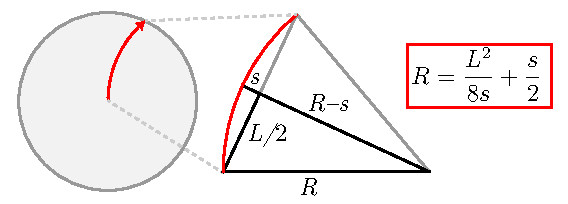
\includegraphics[width=0.8\textwidth]{figures/cms/Sagitta.pdf}
  \caption[Radius of curvature from sagitta.]{Radius of curvature from sagitta. On the left is a depiction of a charged particle leaving a circular arc (red) in the CMS tracker (gray). The length of the chord is $L$, which is also typically the radius of the tracker. The sagitta $s$ is approximately inversely proportional to the radius of curvature $R$, with important consequences for the uncertainty in the desired \pT measurement.}
  \label{cms:sagitta}
\end{figure}
Then $R$, the radius of curvature, can be computed from $L$ and $s$ as follows:
\begin{equation}
  R = \frac{L^2}{8s} + \frac{s}{2} \approx \frac{L^2}{8s}
  \label{cms:eqn_sagitta}
\end{equation}
Since $s$ is typically small compared to $L$, the $s/2$ term can be dropped.
Then $q/\pT$ is approximately proportional to $s$:
\begin{align}
  \frac{q}{\pT} = \frac{1}{BR} \approx \frac{8s}{BL^2}
  \label{cms:pTError}
\end{align}
Since $s$ is linear in the position measurements, its distribution is also Gaussian, and therefore it is the distribution of $q/\pT$, and not $\pT$, that is Gaussian.
The uncertainty on a measurement of \pT obtained from applying standard error propagation to $q/\pT$ must therefore be considered carefully, as it does not describe standard deviations of a variable distributed as a Gaussian.

\subsection{Muon System}
As mentioned in \Sec~\ref{cms:intro}, muon detection is a powerful tool for studying high-energy processes in the presence of high background.
Because of the amount of material in the inner subsystems, typically mostly muons travel through the solenoid.
A track in the muon system therefore is associated with a muon.
Hadronic ``punchthrough'' in the muon system is minimal.

The muon system has three tasks: triggering (\Sec~\ref{cms:trigger}), muon identification, and muon reconstruction.
As with the other subsystems, the shape of the solenoid informs a design of a cylindrical barrel section and an endcap disk section.
Both sections consist of four stations of muon detectors, concentric for the barrel and sequential for the endcap.
The muon system consists of three kinds of gaseous ionization detectors: drift tubes (DT), cathode strip chambers (CSC), and resistive plate chambers (RPC).

The chambers of the muon system are embedded within a set of steel disks in the endcap and concentric twelve-sided steel cylinders in the barrel, referred to as the return yoke.
The return magnetic flux of the solenoid is mostly contained within this return yoke \cite{Chatrchyan:2008zzk, CMS:1997dma}.

\subsubsection{Drift Tubes}
The barrel region of the muon system consists of four stations instrumented with 250 drift tube chambers.
Drift tubes were chosen to be the tracking detectors in the barrel region in light of the low expected rate and relatively low intensity of the local magnetic field.
\Fig~\ref{cms:dt} is a diagram showing the principle of operation of a drift tube cell.
A cathode tube with cross-sectional dimensions $42 \mm \times 13 \mm$ contains an anode wire (operating at 3600\unit{V}) under tension.
The tube is filled with a gas mixture of 85\% Ar and 15\% CO$_2$.
An energetic muon passing through this cell ionizes the gas, and the resulting electrons drift towards the wire.
Measuring the drift time (a maximum of 380\unit{ns}) yields a measurement of position within the cell.

The smallest independent unit of a DT is a superlayer (SL), consisting of four layers of drift cells staggered by a half cell.
A drift tube chamber consists of three (or two) SLs.
The wires in the two outer SLs are parallel to the beam line, and provide a track measurement in the $r$-$\phi$ (bending) plane.
The wires in the inner SL are orthogonal to the beam line, and measure the $z$-position along the beam.
This inner SL is not present in the fourth muon station, which consequently only measures the $\phi$ coordinate.

\begin{figure}[tpb]
  \centering
  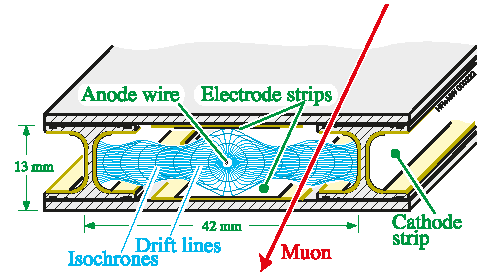
\includegraphics[width=0.8\textwidth]{figures/cms/DT.pdf}
  \caption[Principle of operation of a drift tube cell.]{Principle of operation of a drift tube cell, reproduced from Reference~\cite{Chatrchyan:2013sba}, showing the structure of a cell, as well as the drift lines and isochrones.}
  \label{cms:dt}
\end{figure}

\subsubsection{Cathode Strip Chambers}
The endcap region of the muon system consists of four stations instrumented with 540 cathode strip chambers.
Cathode strip chambers were chosen to be the tracking detectors in the endcap region for their excellent position resolution in the $\phi$ direction achieved by precision cathode charge readout and interpolation.
The CSCs are arranged in circular disks.
Each CSC consists of six layers, each layer lying in an $r$-$\phi$ plane of CMS, consisting of a gas mixture of 50\% CO$_2$, 40\% Ar, and 10\% CF$_4$ in between a plane of copper cathode strips and a plane of anode wires, operating at 2900--3600\unit{V}.
An energetic muon passing through a CSC ionizes the gas, and the resulting electrons drift towards the wires, causing an avalanche of charge that induces an opposite charge on the cathode strips.
Interpolating these charges yields a precise localization of the avalanche.
A more detailed overview of CSCs in the context of a study of neutron-induced background is given in \Sec~\ref{sec:csc_electronics}.

\subsubsection{Resistive Plate Chambers}
Interspersed throughout both the barrel and endcap muon system are 480 and 576 resistive plate chambers, respectively, whose purpose is a fast time response and resolution comparable to that of scintillators.
RPCs therefore are part of a dedicated muon trigger for identifying muon tracks and assigning the bunch crossing with high efficiency.
An RPC consists of two parallel plates of phenolic resin coated with conductive graphite, with a 2\mm gap filled with a gas mixture of 95.2\% freon (C$_2$H$_2$F$_4$, known as R134a), 3.5\% isobutane (i-C$_4$H$_{10}$), and 0.3\% sulfur hexafluoride (SF$_6$).
An energetic muon crossing the chamber ionizes the gas and induces an image charge, which is sampled and read out.
The RPCs have a time resolution of about 2\unit{ns}, a much shorter time than the 25\unit{ns} between LHC bunch crossings, but much coarser position resolution than DTs or CSCs.

\subsubsection{Muon Momentum Resolution}
An important consequence of a dedicated muon system for reconstructing muons is that it improves the \pT resolution for muons at high muon \pT.
\Fig~\ref{cms:muonpT} shows plots of the muon \pT resolution using the inner tracking system only, using the muon system only, and combining both, as a function of \pT.
At lower \pT values, the tracker is sufficient to precisely measure the curvature of the muon track, and the tracker-only resolution dominates.
But at higher \pT values, the tracker track is much straighter, and the additional information about muon position obtained from the muon system results in a \pT resolution superior to that obtained by using either system alone.

\begin{figure}[tpb]
  \centering
  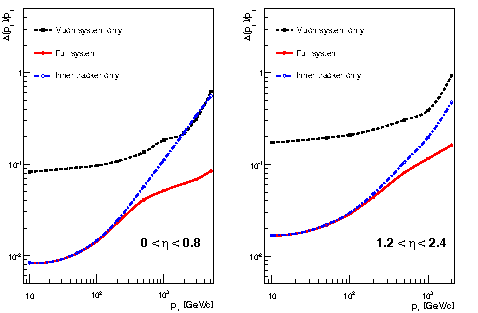
\includegraphics[width=\textwidth]{figures/cms/MuonMomentumResolution.pdf}
  \caption[Muon \pT resolution as a function of muon \pT for the barrel and endcap using the tracking system only, muon system only, and combining both.]{Muon \pT resolution as a function of muon \pT, for (left) the barrel and (right) the endcap, using the inner tracking system only, using the muon system only, and combining both. Reproduced from Reference~\cite{Chatrchyan:2008zzk}.}
  \label{cms:muonpT}
\end{figure}

\subsection{Trigger System}
\label{cms:trigger}
The LHC provides \pp collisions every 25\unit{ns}, corresponding to a crossing frequency of 40\unit{MHz}.
It is impossible to process and store this large amount of data synchronously with such a high rate, and so a rate reduction must be achieved, selecting a subset of the most interesting candidate events for physics analysis.
This rate reduction is performed by the CMS trigger system, an elaborate system of hardware and software that analyzes every bunch crossing and ``triggers'' on potentially interesting events.
The CMS trigger system operates in two steps.
The Level-1 (L1) trigger makes its decisions at the hardware level with custom-built programmable electronics, synchronously with the LHC, and is designed to reduce the rate from 40\unit{MHz} to 100\unit{kHz}.
The High-Level Trigger (HLT) makes its decisions at the software level, performing its computations in real time with respect to the full rate of the LHC, using a processor farm located on the surface at Point~5.
HLT processing operates more slowly than the L1 trigger, but faster than the full event readout, serving to reduce the rate from 100\unit{kHz} to the data acquisition rate of hundreds of Hz \cite{Chatrchyan:2008zzk, Adam:2005zf}.

The L1 trigger consists of a muon trigger and a calorimeter trigger, organized into local, regional, and global components.
Both the ECAL and all components of the HCAL participate in the calorimeter trigger, and all three muon chambers---DTs, CSCs, and RPCs---participate in the muon trigger, the first muon trigger to measure momentum at the hardware Level-1.
The local components are the lowest level, based on energy deposits in the calorimeters and hits and segments in the muon system.
Regional components combine the information from the local components using pattern recognition and track finding and rank trigger objects in small regions.
The global components determine the highest-rank objects and transfer them to the global trigger of the L1 system.
The global trigger then makes the decision to reject or accept the event at Level-1.
A Level-1 Accept (L1A) decision is communicated to the subsystems and the event is passed to the HLT for further evaluation.
The L1 trigger must analyze every bunch crossing, doing so with a maximum latency of 3.2\mus.
\Fig~\ref{cms:L1} depicts the architecture of the L1 trigger.

\begin{figure}[tb]
  \centering
  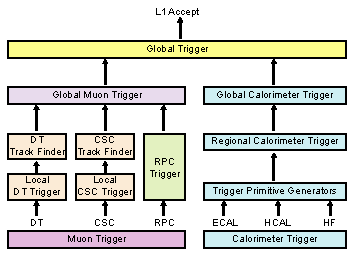
\includegraphics[width=0.8\textwidth]{figures/cms/L1Architecture.pdf}
  \caption[Architecture of the L1 trigger system, depicting the local, regional, and global components of the muon and calorimeter triggers.]{Architecture of the L1 trigger system, based on a figure from Reference~\cite{Chatrchyan:2008zzk}, depicting the local, regional, and global components of the muon and calorimeter triggers, the information from which is processed by the global L1 trigger for trigger decision at L1.}
  \label{cms:L1}
\end{figure}

\pagebreak
The L1 and HLT menus consists of paths that define criteria on which to trigger.
These criteria are the first step to any physics analysis, and so can include requirements on \pT, on numbers of muons or jets, on the geometry and angles between them, and much more.
The HLT uses information from the entire detector, with high-level algorithms that make a more precise decision than the coarser L1 trigger.
Each HLT path is seeded by one or more L1 paths and is designed to be inclusive and general while keeping the event rate in the data acquisition system within its maximum rate.


\chapter{Displaced dimuons}
Displaced dimuons

%%%%%
\chapter{Neutron-Induced Background Hits in the CMS Endcap Muon System and Implications for the HL-LHC}
\label{chap:neutron}
\section{Foreword}
The work presented here was presented at the 2017 European Physical Society Conference on High-Energy Physics (EPS-HEP) and the 2017 American Physical Society Meeting of the Division of Particles \& Fields (APS-DPF). The EPS-HEP poster can be found at Reference~\cite{Dasgupta:Poster}, the associated proceedings can be found at Reference~\cite{Dasgupta:Proceedings}, the APS-DPF parallel talk can be found at Reference~\cite{Schnaible:Talk}, and the public repository of approved plots can be found at Reference~\cite{NeutronTwiki}. The text and plots were written and produced together with Christian Schnaible and Bob Cousins and form the internal detector note CMS DN-2017/019.

\section{Introduction}
\label{sec:intro}
The high-luminosity upgrade to the CERN LHC (HL-LHC) will bring not only increased access to discovering new physics but also increased background rates in CMS muon chambers \cite{Evans:2008zzb,Apollinari:2116337}. This note focuses on the study of neutron-induced background hits in CMS endcap cathode strip chambers (CSCs) due to their large active volume and forward placement in CMS \cite{CMS:1997dma,Chatrchyan:2009hb}. Neutrons induce hits in CSCs by producing photons, via either nuclear scattering or capture. These photons produce or scatter electrons, via Compton scattering, the photoelectric effect, or pair production; the ionization from these electrons can either corrupt hits from desirable tracks in the event, or add extra background hits. This note describes efforts to quantify and characterize the effects of this neutron-induced ionization through analysis of Monte Carlo (MC) simulation of neutron production and propagation in CMS, as well as of CMS proton-proton (\pp) collision data. The results are tied to analyses of muon test beam data at the CERN Gamma Irradiation Facility (GIF++), which allows us to study the effects of background radiation on CSC performance and project the effects of neutron-induced background to the conditions at the HL-LHC.

In the debris of \pp collisions, hadronic interactions liberate neutrons from CMS calorimeters, shielding, and various other detector structures. These neutrons can carry several \GeVns or more of kinetic energy, propagating throughout the experimental cavern, detector materials, and shielding. They lose kinetic energy through many scattering interactions over the course of several milliseconds, and if not captured sooner, are eventually cooled to thermal equilibrium with the cavern environment, carrying kinetic energies of around 0.025\unit{eV} (300\unit{K}). There are three main processes by which neutrons lead to photons: inelastic scattering, resonant capture on nuclei, and thermal capture on nuclei \cite{Kopecky:1997}.

Neutrons with several \MeVns of kinetic energy may scatter inelastically with detector and shielding material, producing one or more photons. In addition to undergoing inelastic scattering, neutrons may be captured by various nuclei, including iron, copper, and free hydrogen, resulting in excited isotopes of the original capturing nuclei with energies typically a few \MeVns greater than that of their ground states. The excited isotopes reach their ground states by emitting one or more photons. Resonant capture occurs when the kinetic energy of a neutron (typically of order \keVns) is such that the sum of the total neutron and target nucleus energies matches the total energy of a discrete excited state of the final-state isotope. For example, \chem{56}{Fe} has a resonant neutron capture cross section at a neutron kinetic energy of 1.1\keV \cite{Kopecky:1997}. Thermal capture occurs when neutrons have reached sub-eV thermal energies, in a regime where the cross section for capture increases with decreasing neutron velocity. Throughout this note, any reference to neutron capture refers to both thermal and resonant neutron capture unless otherwise specified. 

The photons produced from inelastic scattering and nuclear capture are typically of order \MeVns in energy. Once produced, the photons can propagate inside the gas volume of a CMS CSC where they predominantly scatter off electrons, but also produce electrons via pair production and the photoelectric effect. These scattered electrons can ionize the chamber gas and subsequently lead to background hits.

Such hits constitute an important source of background rates as well as contribute to aging of muon chambers. This note focuses on the effect that these increased background rates have on muon triggering and offline reconstruction of muons and measurement of their properties. 

The identification of neutron-induced hits in CMS data is complicated by the fact that data from a CSC is read out only if the CSC trigger electronics identify a potential muon track (trigger primitive) in that CSC \cite{Hauser:814259,Acosta:2002km,Acosta:200826}. A muon leading to a trigger primitive can induce other hits in the CSC via \eg bremsstrahlung or delta rays, or be accompanied by other charged particles from a jet in which the muon is embedded. Precision measurements of the ionization charge are read out through the main CMS data acquisition (DAQ) system only for a small fraction of the area of the CSC that is near the muon that generated the trigger, and are particularly vulnerable to hits from these extra particles. Thus, for most of the studies in this paper, we use instead the diagnostic information for the whole chamber that is passed to the DAQ by the trigger electronics (the so-called ``trigger path''). These trigger path data are much less precise than the high-precision charge data read out by the main DAQ \cite{Baarmand:1999ka}, but since they include information from the entire chamber, they allow us to look for neutron-induced hits in areas of the chamber that are further away from the muon that generated the trigger. With various additional selection criteria, sufficient samples of neutron-induced hits are obtained for detailed studies of rates in CMS CSCs, for comparison to simulated CMS data and GIF++ data.

\Sec~\ref{sec:csc_electronics} is a brief overview of cathode strip chambers and the on-chamber trigger electronics in the CMS detector. \Sec~\ref{sec:G4_neutron_sim} describes \GEANTfour simulation of the detector response to \pp collisions, including neutron-induced hits. \Sec~\ref{sec:selection} describes the selection criteria that we use to isolate a sample of neutron-induced hits in CMS CSC data. \Sec~\ref{sec:datamc} describes the procedure by which we normalize our neutron-induced hit counts into hit rates. \Secs~\ref{sec:GIF} and \ref{sec:chargeperhit} describe studies of GIF++ data and CMS CSC data from which we predict some effects of increased radiation in HL-LHC-like conditions. 

\section{Cathode Strip Chambers and Trigger Electronics in CMS}
%\section{Cathode Strip Chambers and Trigger Electronics in the CMS Detector}
\label{sec:csc_electronics}
%\subsection{The CMS Detector}
%The central feature of the CMS apparatus is a superconducting solenoid of 6\unit{m} internal diameter, providing a magnetic field of 3.8\unit{T}. Within the solenoid volume are a silicon pixel and strip tracker, a lead tungstate crystal electromagnetic calorimeter, and a brass and scintillator hadron calorimeter, each composed of a barrel and two endcap sections. Forward calorimeters extend the pseudorapidity coverage provided by the barrel and endcap detectors. Muons are detected in gas-ionization chambers embedded in the steel flux-return yoke outside the solenoid. Muons are measured in the pseudorapidity range $\abs{\eta} < 2.4$, with detection planes made using three technologies: drift tubes, cathode strip chambers, and resistive plate chambers. Matching muons to tracks measured in the silicon tracker results in a relative transverse momentum resolution for muons with $20 <\pt < 100\GeV$ of 1.3--2.0\% in the barrel and better than 6\% in the endcaps, The \pt resolution in the barrel is better than 10\% for muons with \pt up to 1\TeV.

The CSC system in the endcap muon detection system of CMS \cite{Acosta:2002km} contains 540 chambers. Each endcap has 4 stations numbered from 1 to 4, and each station contains two or three rings of chambers. A chamber is uniquely specified by a string of the form ME$\pm S/R/C$, where $\pm$ refers to either the + or $-$ endcap, $S$ is the station number, $R$ is the ring number, and $C$ is the chamber number, \eg ME+1/1/36. Part of this notation may be omitted when referring to groups of chambers; for example, we refer to ME1/1 or ME2/1 chambers, \ie chambers in the innermost ring of the first or second stations, respectively, in either endcap.

\begin{figure}[p]
	\centering
	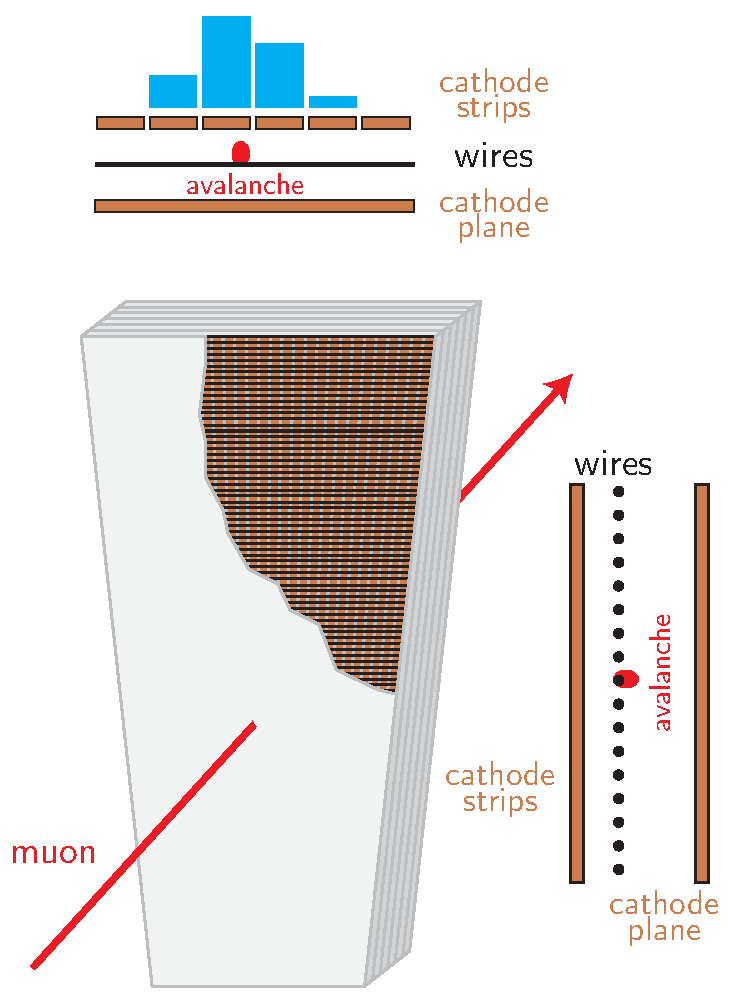
\includegraphics[width=\dummyFigWidth]{figures/neutron/fig_CSC.pdf}
	\caption{Diagram and principle of operation of a CSC endcap muon chamber in CMS.}
	\label{fig:CSC}
\end{figure}

The ring of chambers in each station is perpendicular to the $z$ axis of CMS, with the narrow end of their trapezoidal shapes closer to the beam line. \Fig~\ref{fig:CSC} contains a diagram illustrating the principle of operation of a CSC. Each CSC is a multi-wire proportional chamber consisting of 6 layers, with each layer lying in an $r$-$\phi$ plane of CMS. Each layer contains a gas volume consisting of 50\% CO$_2$, 40\% Ar, and 10\% CF$_4$ in between a plane of copper cathode strips and a plane of anode wires. The strips extend from the narrow end to the wide end, along the $r$ direction, at constant $z$ and $\phi$ coordinates; the wires extend parallel to the narrow and wide ends, approximately along the $\phi$ direction, at constant $z$ and approximately constant $r$ coordinates. The wires are spaced 2.5--3.5\mm apart, arranged in groups of 5--16\mm (wire groups, or WG), and kept at a high voltage of 2900--3600\unit{V} with respect to the cathode strips. 

A muon ionizes the gas, and the resulting electrons drift towards the wires, causing an avalanche of charge that induces an opposite charge on the cathode strips. The notable feature of a CSC is excellent position resolution in the $\phi$ direction achieved by precision cathode charge readout and interpolation. Cathode trigger electronics include a comparator network, which provides half-strip hit position resolution in the trigger hardware. Cathode comparator hits give the layer and half-strip number and anode wire group hits give the layer and wire group number. A digitized detector hit -- a cathode strip hit or a wire group hit -- is referred to as a digi, and therefore the strip (or half-strip) number or wire group number may also generally be referred to as a digi number \cite{Hauser:814259,Baarmand:1999ka,Acosta:200826}.

\begin{figure}[p]
	\centering
	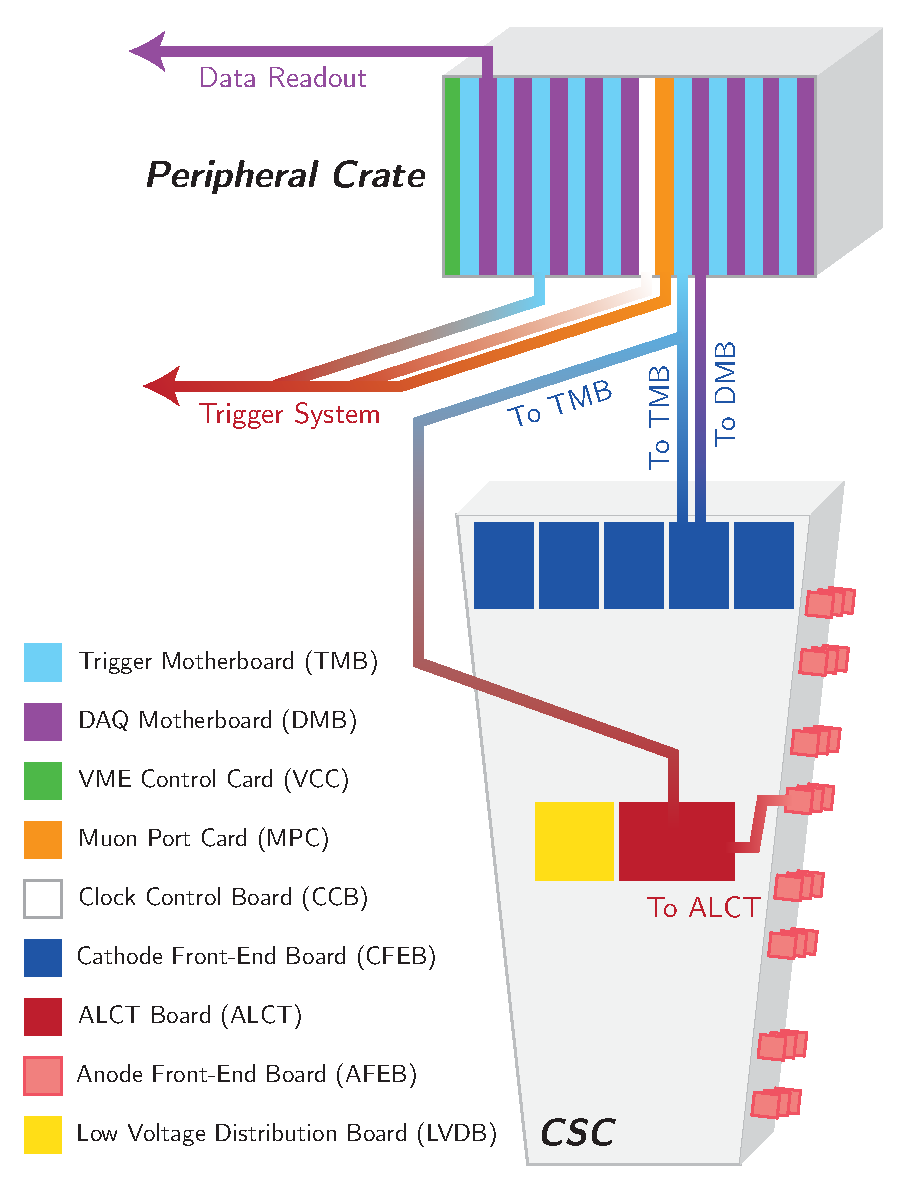
\includegraphics[width=\dummyFigWidth]{figures/neutron/fig_CSC_electronics.pdf}
	\caption{Diagram of the CSC electronics system in CMS.}
	\label{fig:CSC_electronics}
\end{figure}

As illustrated in \FigDot~\ref{fig:CSC_electronics}, the anode wire group hits and comparator half-strip hits are transmitted to circuits that perform low-level local pattern recognition on the hits in the six layers of a chamber. Candidate tracks from charged particles are identified separately in the cathode strips and anode wires and then combined. Anode local charged tracks (ALCTs) are formed by ALCT boards, which receive data for each plane from anode front end boards (AFEBs). Cathode local charged tracks (CLCTs) are formed in two steps within the trigger motherboard (TMB) from data transmitted by cathode front end boards (CFEBs). First, a set of loose requirements, for example on the number of layers hit, are applied to the CFEB data. These are known as the pre-trigger, and a candidate track that passes these requirements is called a pre-CLCT. Then, a set of tighter requirements are applied, and a pre-CLCT that passes these requirements becomes a CLCT. The TMB also receives ALCTs from the ALCT boards and combines coincident ALCTs and CLCTs to create local charged tracks (LCTs). The CSC electronics firmware has programmable requirements for the various pattern recognition steps, \eg for the number of layers hit, the spatial distribution of the hits, the temporal distribution of the hits, and the time window for coincidence of the ALCTs and CLCTs. 

These trigger data, referred to as trigger primitives, are transmitted to the endcap muon trigger system and also inserted into the DAQ stream via the DAQ motherboard (DMB). For offline use, the DMB also reads out the high-precision analog-to-digital converter (ADC) charge measurement for each cathode strip when the DMB receives a signal from the CMS \Lone trigger. However, these ADC charge measurement data are read only from CFEBs for which a pre-CLCT was formed, which correspond to only a fraction of a chamber. As noted above, muon-induced background hits make these data of limited use in our current studies of neutron-induced hits.

The data from the TMB contains both early and late detector hits with respect to the muon that generated the trigger are inserted into the DAQ stream. Hit times are binned into 16 readout time bins of 25\unit{ns} each, with the muon usually inducing hits in time bins 7 or 8. The chamber electronics can thus read out detector hits that occur approximately 200\unit{ns} (8 time bins) before and after the muon hits.

\section{\GEANTfour MC Simulation for Neutron Studies}
\label{sec:G4_neutron_sim}
\subsection{\GEANTfour MC Simulation Setup}
To better understand the basic nuclear interactions that may result in background hits in CSCs, we turn to simulation. We used the \GEANTfour simulation package to simulate minimum-bias proton-proton (\pp) collision events \cite{Agostinelli:2002hh,Allison:2006ve,Allison:2016lfl,Sjostrand:2006za}. To study neutron background effectively, a few specific modifications to the default CMS simulation configurations were necessary~\cite{PietsPage};

\begin{figure}[htbp]
	\centering
	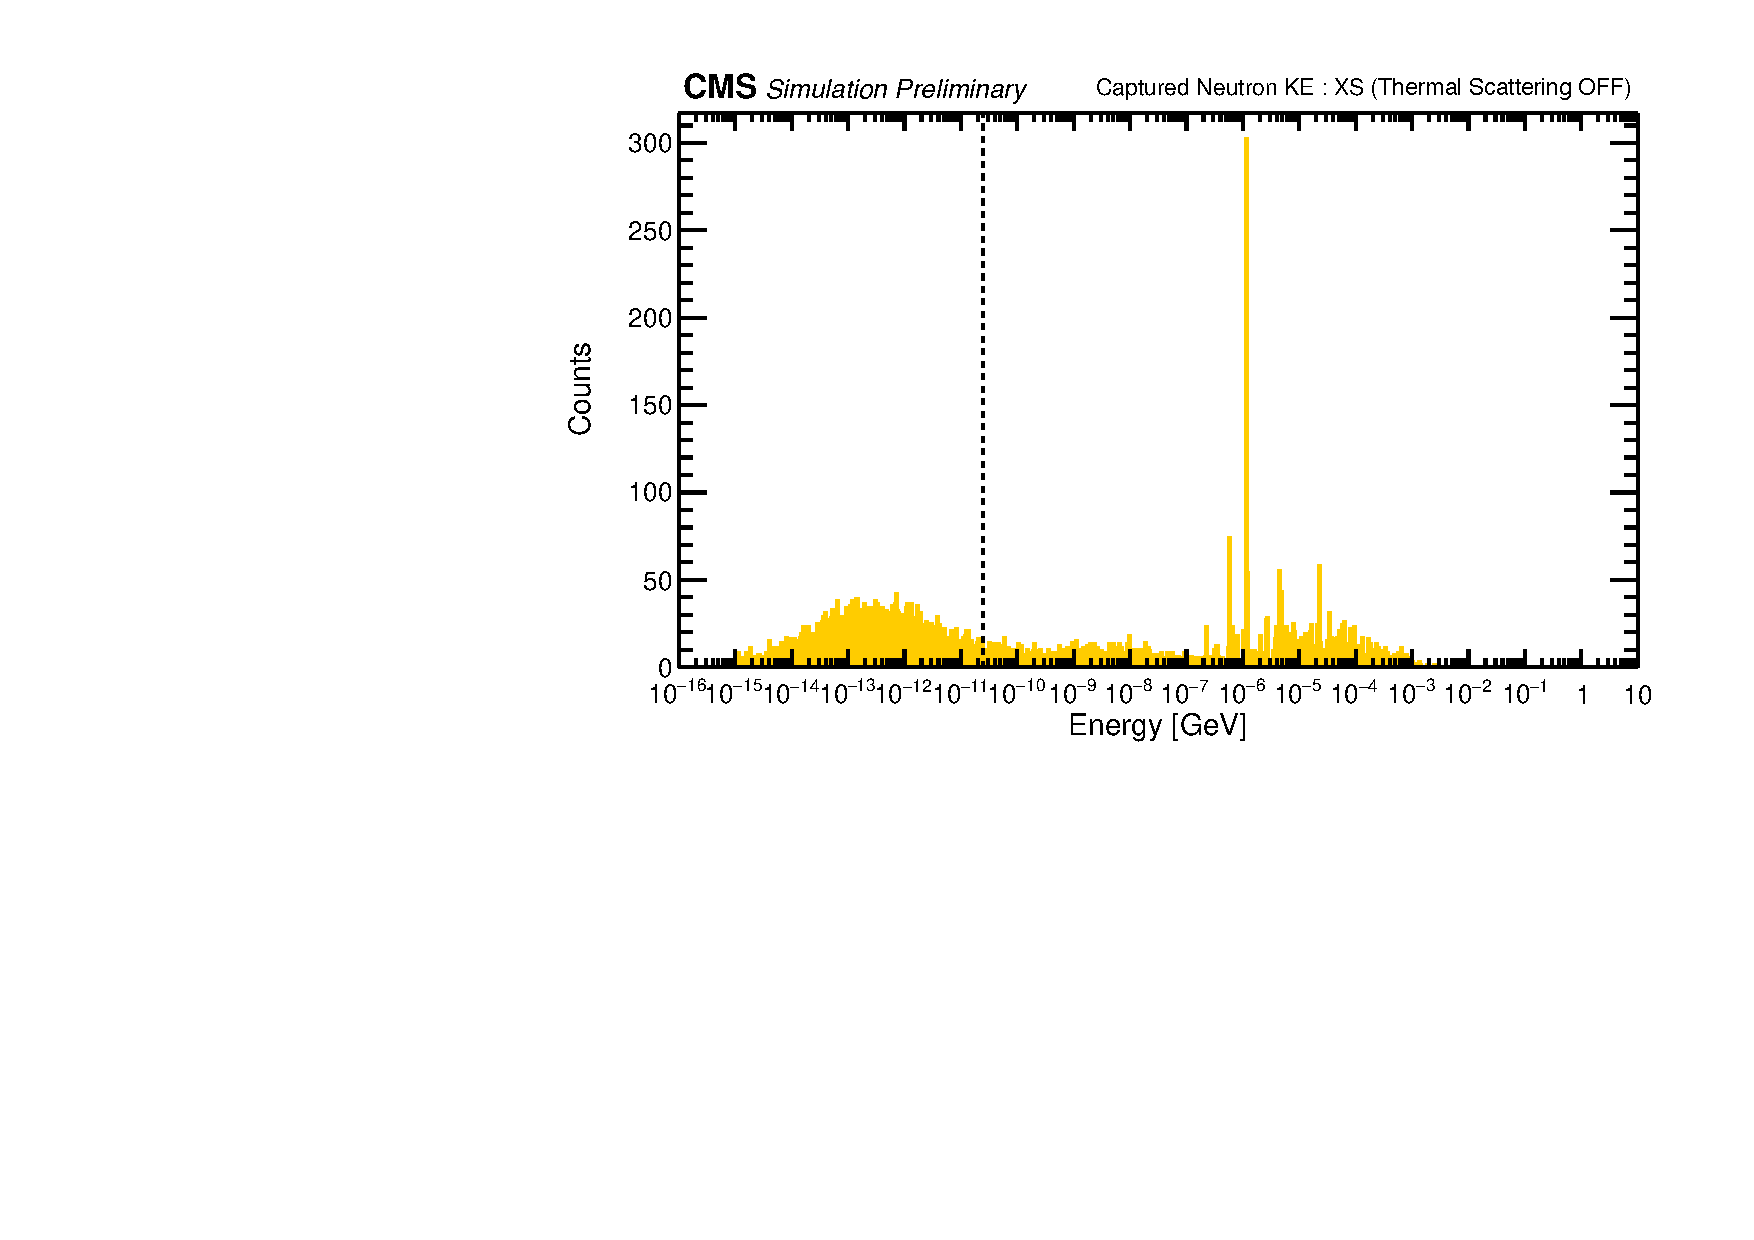
\includegraphics[width=\dummyFigWidth]{figures/neutron/neutronSpectrum_before.pdf}\\
	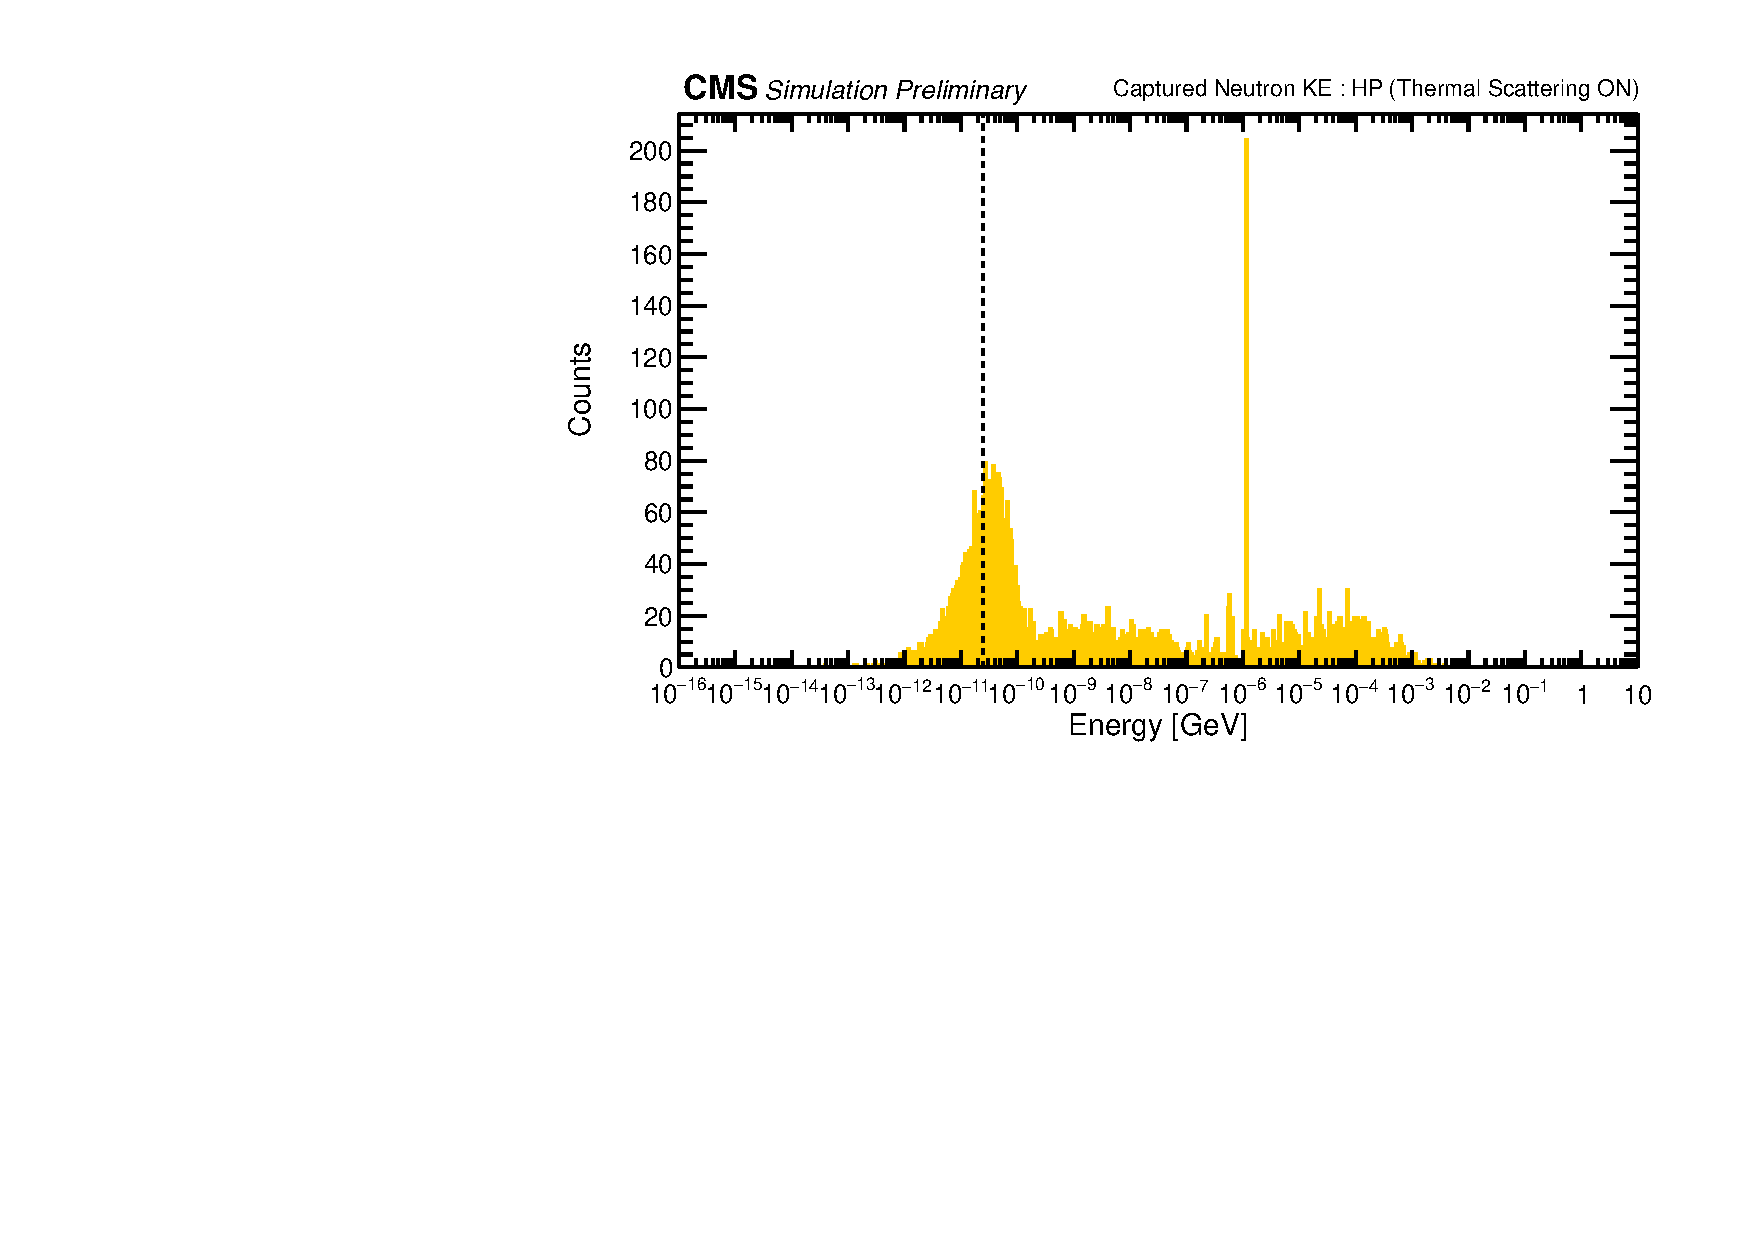
\includegraphics[width=\dummyFigWidth]{figures/neutron/neutronSpectrum_after.pdf}
  \caption[Histogram of neutron kinetic energy just before nuclear capture, before and after enabling thermal treatment of detector nuclei.]{Histogram of neutron kinetic energy just before nuclear capture, (\posstyle{top}) before and (\posstyle{bottom}) after enabling thermal treatment of detector nuclei. The dashed line indicates 0.025\unit{eV}. Before enabling the new feature, the low energy peak of captured neutrons is several orders of magnitude below thermal energies; after enabling the feature, the low energy peak is at thermal energies. Also visible are the resonant capture peaks on, for example, \chem{56}{Fe}, in the \keVns range.}
	\label{fig:nKE}
\end{figure}

\begin{itemize}
	\item To accommodate the long lifetimes of the neutrons under study, we extended the tracking time of all particles to 10\unit{s}.
	\item To accommodate the low energies of the neutrons under study, we removed any particle energy thresholds where they existed.
	\item To properly model low-energy neutrons, we enabled a feature in the \GEANTfour thermal neutron scattering routine that models nuclei at room temperature. The standard \GEANTfour routine models the temperature of the nuclei in the detector at 0\unit{K} and as a result artificially cools neutrons down to well below thermal energies. \Fig~\ref{fig:nKE} displays histograms of the kinetic energy of neutrons just before their capture on a nucleus, before and after the new feature was enabled. The dashed line is at 0.025\unit{eV}; without the feature enabled, the low energy peak of captured neutrons is well below thermal energies, whereas with it enabled, the low energy peak is at thermal energies.
	\item To retain all electronics signals in simulated CSCs, we assigned simulated hits produced after times longer than 200\unit{ns} a time of 200\unit{ns} in the CSC digitization simulation module. This is to ensure that all hits from a single simulated \pp collision are retained, rather than just the hits that occur within the simulated detectors' limited time readout window of 400\unit{ns}.
\end{itemize}

Two versions of \GEANTfour neutron interaction packages are compared:

\begin{itemize}
	\item HP: ``High Precision'' package that parametrizes existing experimental nuclear data for neutron interaction cross sections, and
	\item XS: intended for CPU time optimization, derived from HP by approximating detailed parameterizations in HP with averages.
\end{itemize}

\subsection{Results from MC Simulation}
In examining these simulated events, we find that each \pp collision can lead to three broad categories of neutron-induced hits:

\begin{itemize}
	\item Hits on the time scale of 100\unit{ns} after the \pp collision, induced by ``fast'' neutrons whose energies have degraded over time to a few \MeVns. The neutrons interact inelastically with nuclei, resulting in some ionization from protons or nuclear fragments, but primarily resulting in nuclear de-excitation photons that give rise to ionizing electrons, primarily from Compton scattering.

	\item Hits on the time scale of several\mus after the \pp collision, induced by neutrons whose energies have degraded over time to energies of a few \keVns. The neutrons are resonantly captured on various types of nuclei, also resulting in nuclear de-excitation photons that give rise to ionizing electrons.

	\item Hits on the time scale of several ms or longer after the \pp collision, induced by thermal neutrons whose energies have degraded over time to be at thermal equilibrium with the experimental cavern. The neutrons are captured on nuclei, also resulting in nuclear de-excitation photons that give rise to ionizing electrons.
\end{itemize}

\begin{figure}[htbp]
	\centering
	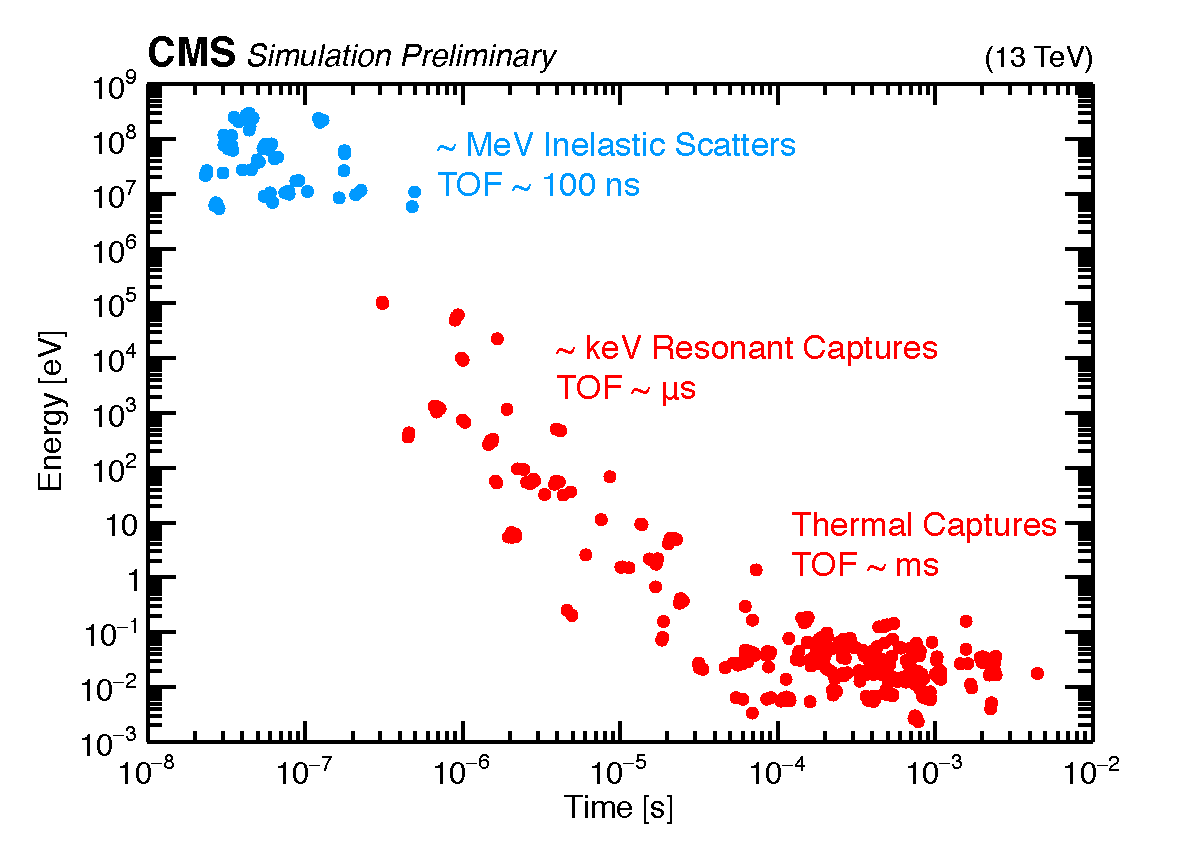
\includegraphics[width=0.8\dummyFigWidth]{figures/neutron/LastEvsTOF.pdf}\\
	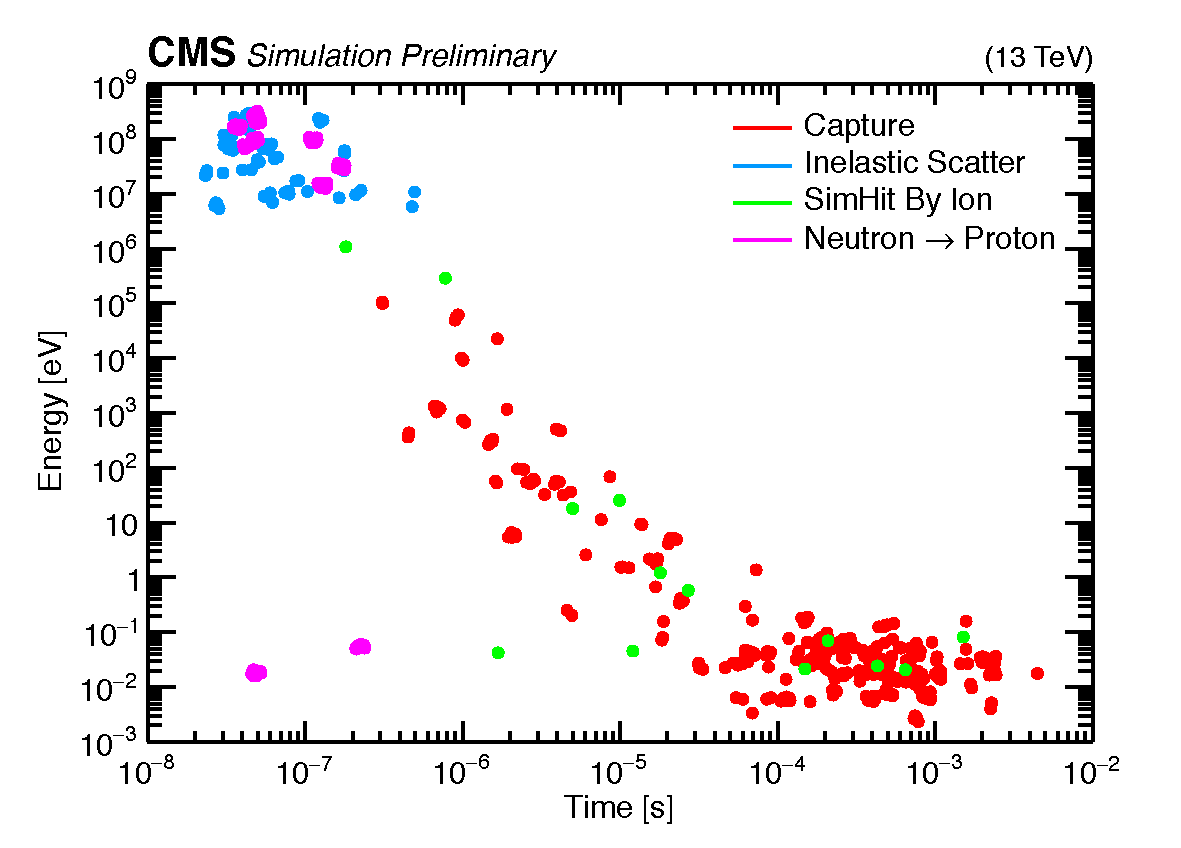
\includegraphics[width=0.8\dummyFigWidth]{figures/neutron/LastEvsTOF_All.pdf}
  \caption[Final energy of simulated neutron \vs the time since \pp collision giving rise to simulated detector hit, for hits in CSCs.]{Final energy of simulated neutron \vs the time since \pp collision giving rise to simulated detector hit, for hits in CSCs. Hits are induced by electrons that are produced from photons that are produced from neutron capture or from neutron inelastic scattering. Red dots indicate simulated hits induced by neutron captures, and blue dots indicate simulated hits induced by neutron inelastic scatters. The top plot shows hits from photons only, coming from inelastic scattering and nuclear capture; the bottom plot shows all neutron-related hits, including those induced by protons and nuclear fragments, shown in magenta and green dots, respectively.}
	\label{fig:tof_energy}
\end{figure}

\Fig~\ref{fig:tof_energy} displays plots of the final energy of simulated neutrons \vs the time (since the \pp collision) of the corresponding simulated detector hits (SimHits) in CSCs. The final energy of the neutron refers to the energy of the neutron at the moment it gives rise to the photon that eventually gives rise to the electron that produced the SimHit. Visible on the top plot are the three categories of hits as mentioned above: two groups of red dots that are hits induced by neutron captures; and blue dots that are hits induced by neutron inelastic scatters. The bottom plot in \FigDot~\ref{fig:tof_energy} shows the same quantities for all neutron-related SimHits, including the photon-induced hits as well as hits from ions (green) and protons (magenta).

Since the time scales from when the neutrons are created to when neutron capture induces hits are much longer than time scales of LHC bunch train gaps \cite{Evans:2008zzb}, hits occur in chambers uniformly at all times during an LHC fill. In simulation, we distinguish thermal neutron capture-induced hits in CSCs from prompt and fast neutron-induced hits by selecting the simulated hits that occur after a sufficiently long time after the \pp collision. 

\begin{figure}
	\centering
	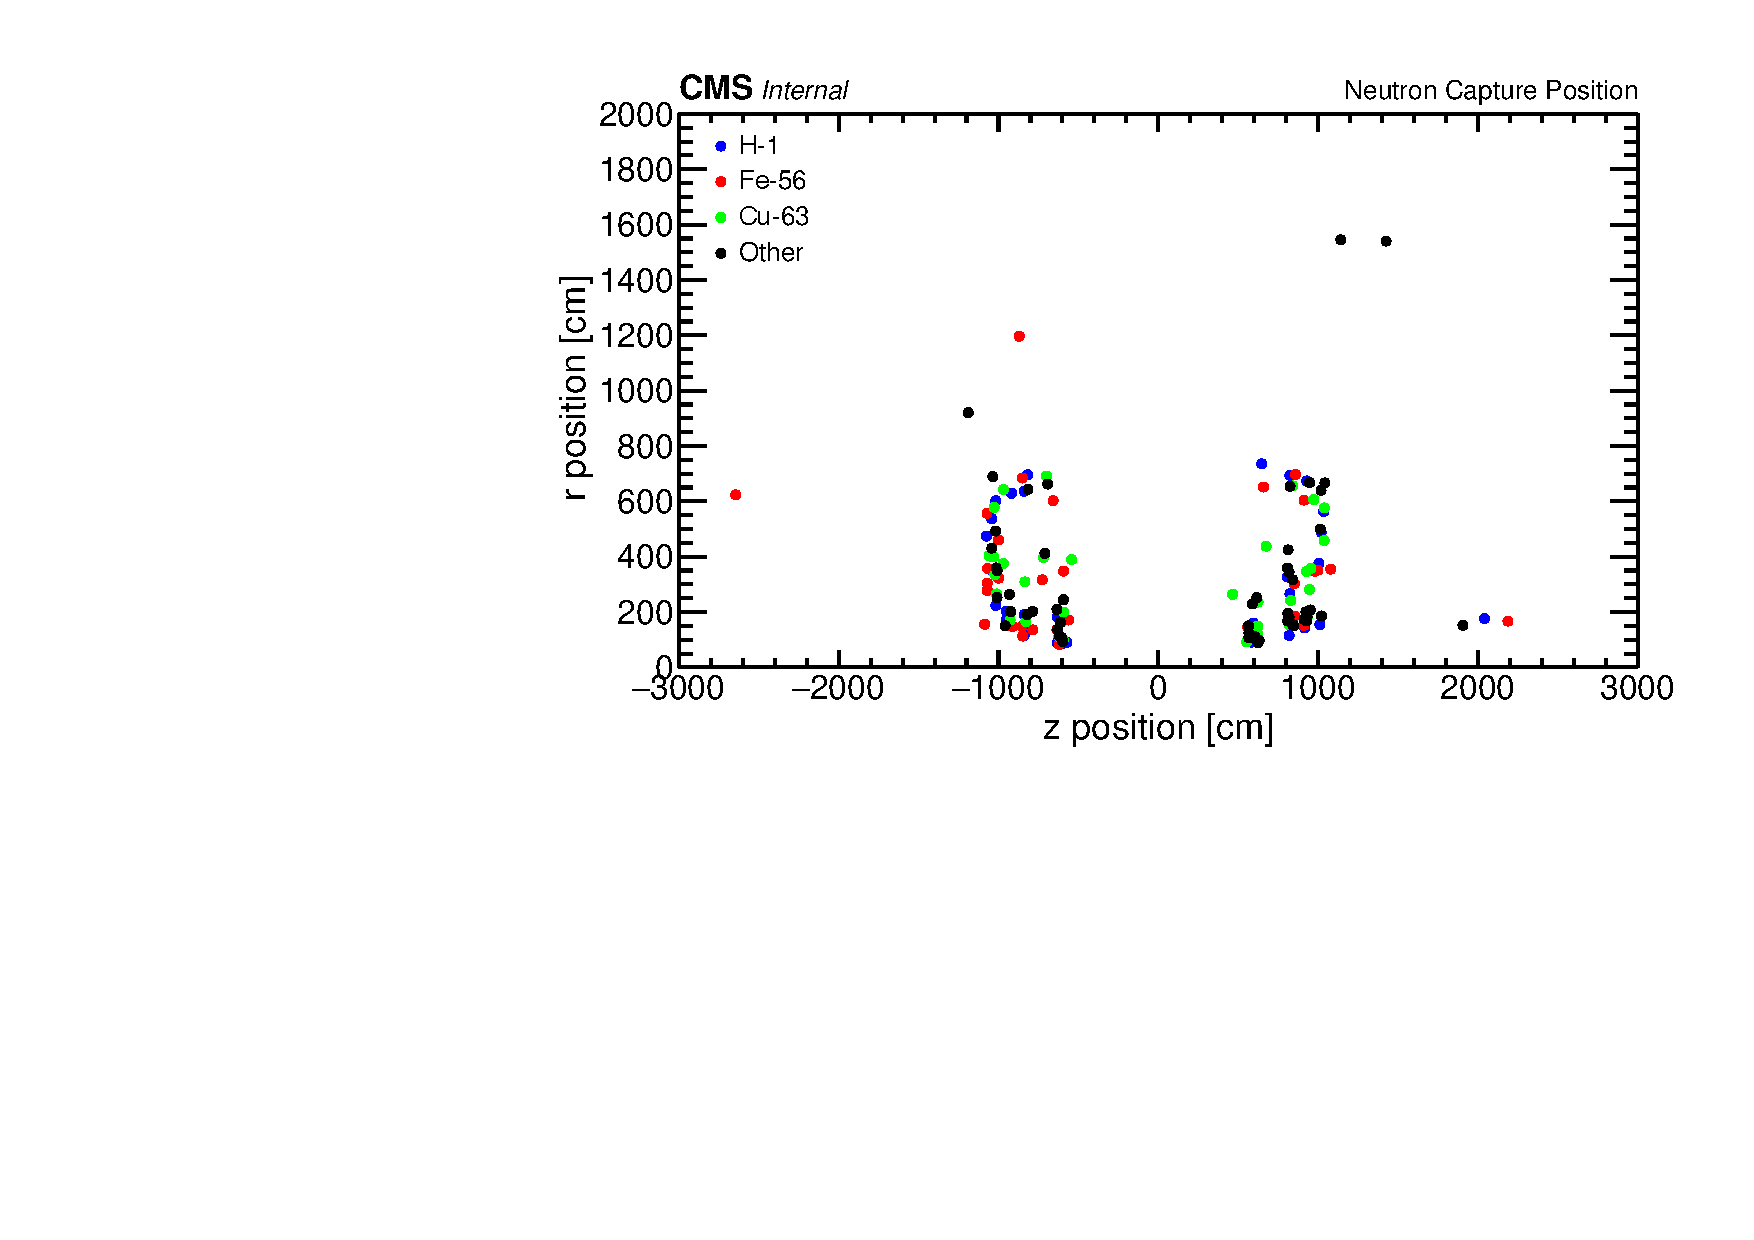
\includegraphics[width=\dummyFigWidth]{figures/neutron/hrzTot_sim_nCapture.pdf}
	\caption{$r$-$z$ view of CMS cavern showing the locations of the specific neutron captures that led to SimHits in the CSCs.}
	\label{fig:hrz_neutron_cap}
\end{figure}

\Fig~\ref{fig:hrz_neutron_cap} is an $r$-$z$ view of the CMS cavern showing the location of neutron captures that lead to SimHits in the CSCs, each dot colored according to the capturing nucleus. Neutrons are mainly captured on \chem{56}{Fe} (red), \chem{63}{Cu} (green), and \chem{1}{H} (blue) within the CMS endcap muon system, CMS calorimeters, and LHC shielding.

\begin{figure}[htbp]
	\centering
	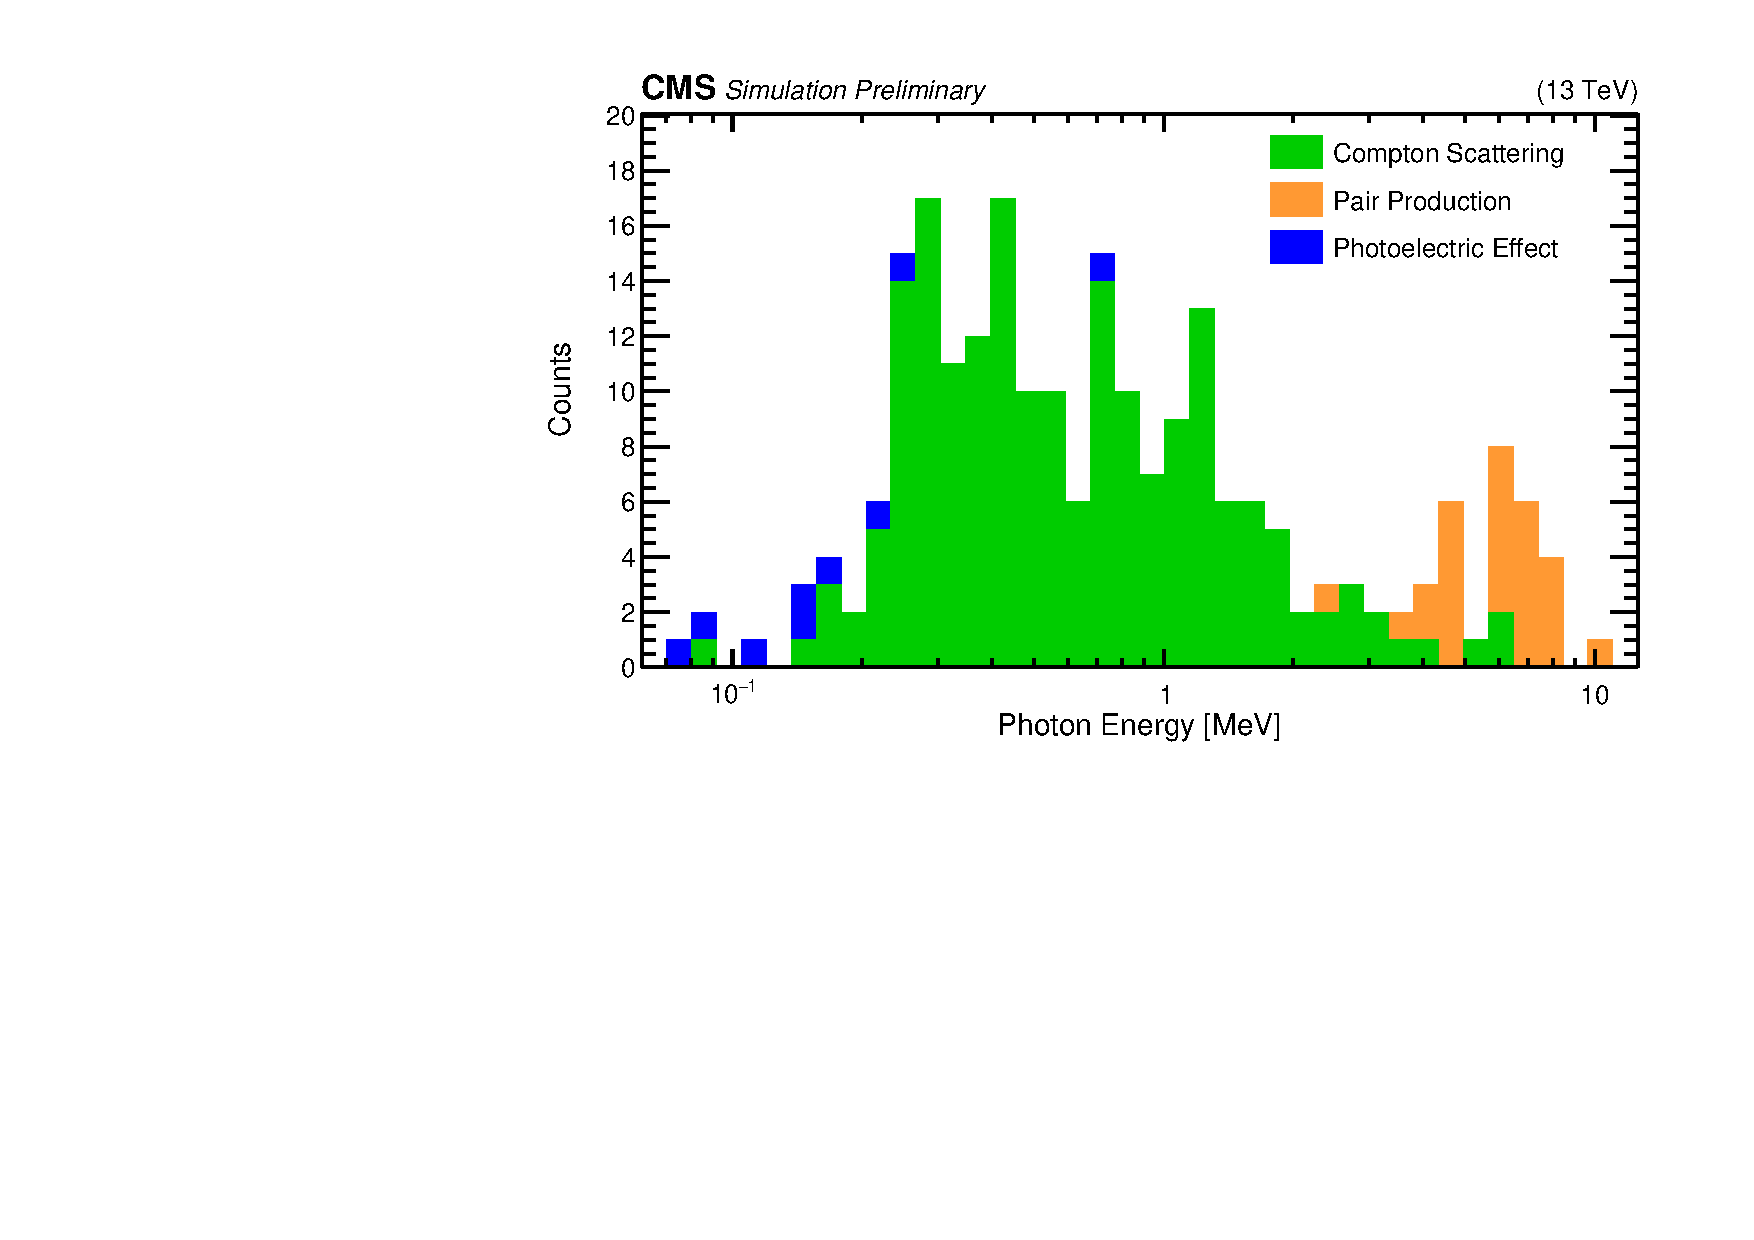
\includegraphics[width=\dummyFigWidth]{figures/neutron/neut_gamma_proc_energy.pdf}
  \caption[Stacked histogram of the final energy of simulated photons at the time they produce simulated electrons that lead to simulated detector hits.]{Stacked histogram of the final energy of simulated photons at the time they produce simulated electrons that lead to simulated detector hits. The photons are categorized by the process by which the electrons are created or scattered. The most common process by which electrons that eventually lead to simulated hits are formed is Compton scattering.}
	\label{fig:electron_proc}
\end{figure}

Of additional interest are the processes by which photons produce the electrons that result in SimHits. \FigDot~\ref{fig:electron_proc} is a histogram of the simulated photon energy emitted by nuclear de-excitations from both inelastic scattering and neutron capture that lead to SimHits, stacked by the specific production or scattering process that created the ionizing electron. Photons that lead to SimHits predominantly have energies of hundreds of \keVns to several \MeVns, and the most common process that leads to SimHits is Compton scattering.

\section{Selection and Isolation of Neutron-Induced Hits in CMS Data}
\label{sec:selection}
To obtain a sample of events in \pp collision data suitable for studying the neutron background, we first select events with \PZ boson candidates decaying to two opposite sign muons from the SingleMuon dataset from Run 2016H, corresponding to approximately 9\fbinv of integrated luminosity. Events are chosen with at least two muons of opposite sign where the muon leading in \pt is required to have $\pt > 30\GeV$, and the subleading muon is required to have $\pt > 20\GeV$. In addition, muon candidate tracks are required to have at least one hit in the pixel detector, hits in at least six silicon-strip tracker layers, and segments in two or more muon stations. To suppress non-prompt muons, the sum of the \pt of charged tracks within a cone of $\Delta R=0.3$ around the muon is required to be less than 10\% of the muon \pt. Also, the muon is required to have a transverse impact parameter of less than 2\mm and a longitudinal distance of less than 5\mm with respect to the primary vertex. The \PZ boson dimuon candidates are selected within an invariant mass window of 60--120\GeV. We thus obtain a sample of prompt muons with reduced hadronic activity near the muon candidate. Finally, at least one of the muons is required to have passed through at least one CSC, by requiring that an LCT in at least one CSC was matched to the muon candidate track. 

\begin{figure}[htbp]
	\centering
	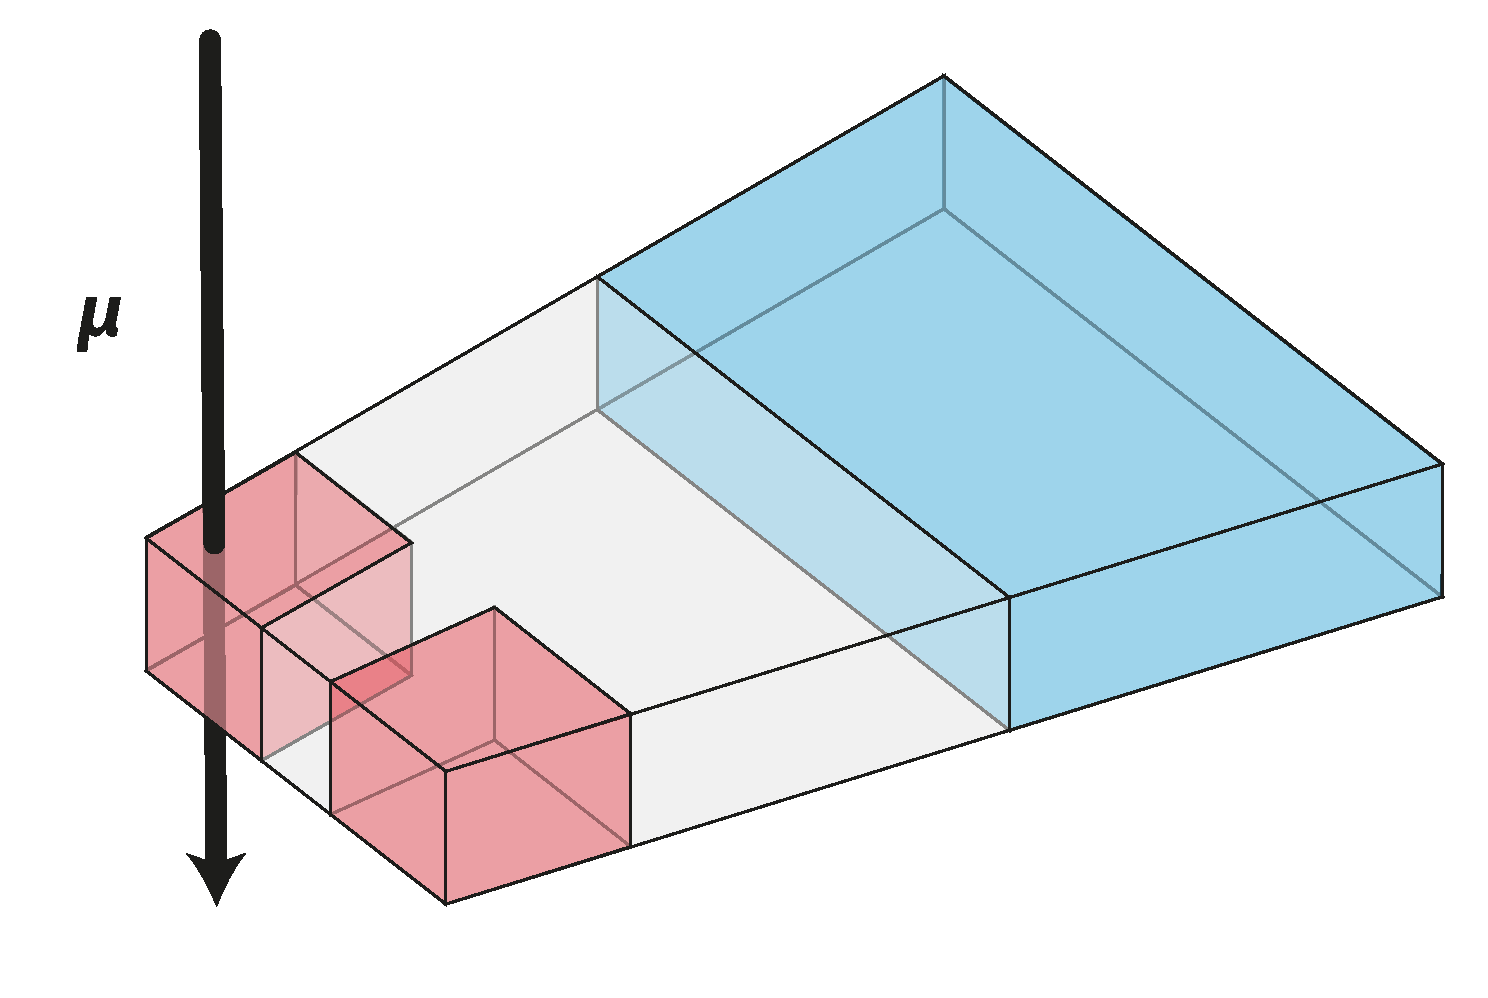
\includegraphics[width=\dummyFigWidth]{figures/neutron/CornerSelection.pdf}
	\caption{Opposite half selection for neutron-induced hits in CSCs.}
	\label{fig:corner}
\end{figure}

We then look for evidence of neutron-induced hits in cathode comparator half-strip hits and anode wire group hits in the data of each CSC thus selected. To reduce potential muon-induced contamination of our selection of candidate neutron-induced hits, we require that there be exactly one LCT occurring in a one-sixteenth corner of a chamber and consider only comparator half-strip or wire group hits occurring in the opposite half of the chamber from the LCT. \Fig~\ref{fig:corner} displays an example diagram of a CSC with a muon (indicated by the black arrow) passing through a chamber corner (shaded in red) and the corresponding opposite half of the chamber (shaded in blue) where we look for hits. This ensures that any potential muon-induced background is at least a quarter chamber spatially separated from the region of the chamber in which we search for candidate neutron-induced hits.

As a precise clarification of what is meant by a one-sixteenth corner and an opposite half, an example definition of a chamber corner area is the overlap region between wire groups 1 through $N_\text{WG} / 4$ and comparator half-strips 1 through $N_\text{HS}/4$, where $N_\text{WG}$ and $N_\text{HS}$ are the total number of anode wire groups and comparator half-strips in a chamber, respectively. The corresponding area for the opposite half of the chamber in which we search for candidate neutron-induced wire group hits is the area defined by wire groups $N_\text{WG}/2$ through $N_\text{WG}$, and similarly for candidate neutron-induced comparator half-strip hits is the area defined by $N_\text{HS}/2$ through $N_\text{HS}$. All four definitions of a chamber corner and their corresponding opposite halves are considered and used in this analysis. 

Since the rate of trigger muons varies over the CSC system, 
the number of times we look in each half-chamber varies for each
half-chamber in the CSCs and for each event, and the hit rates vary with
luminosity. We introduce some rather tedious bookkeeping to
compute rates in the next section, with an indicator function used
to specify when we look.

\begin{figure}[tbp]
	\centering
	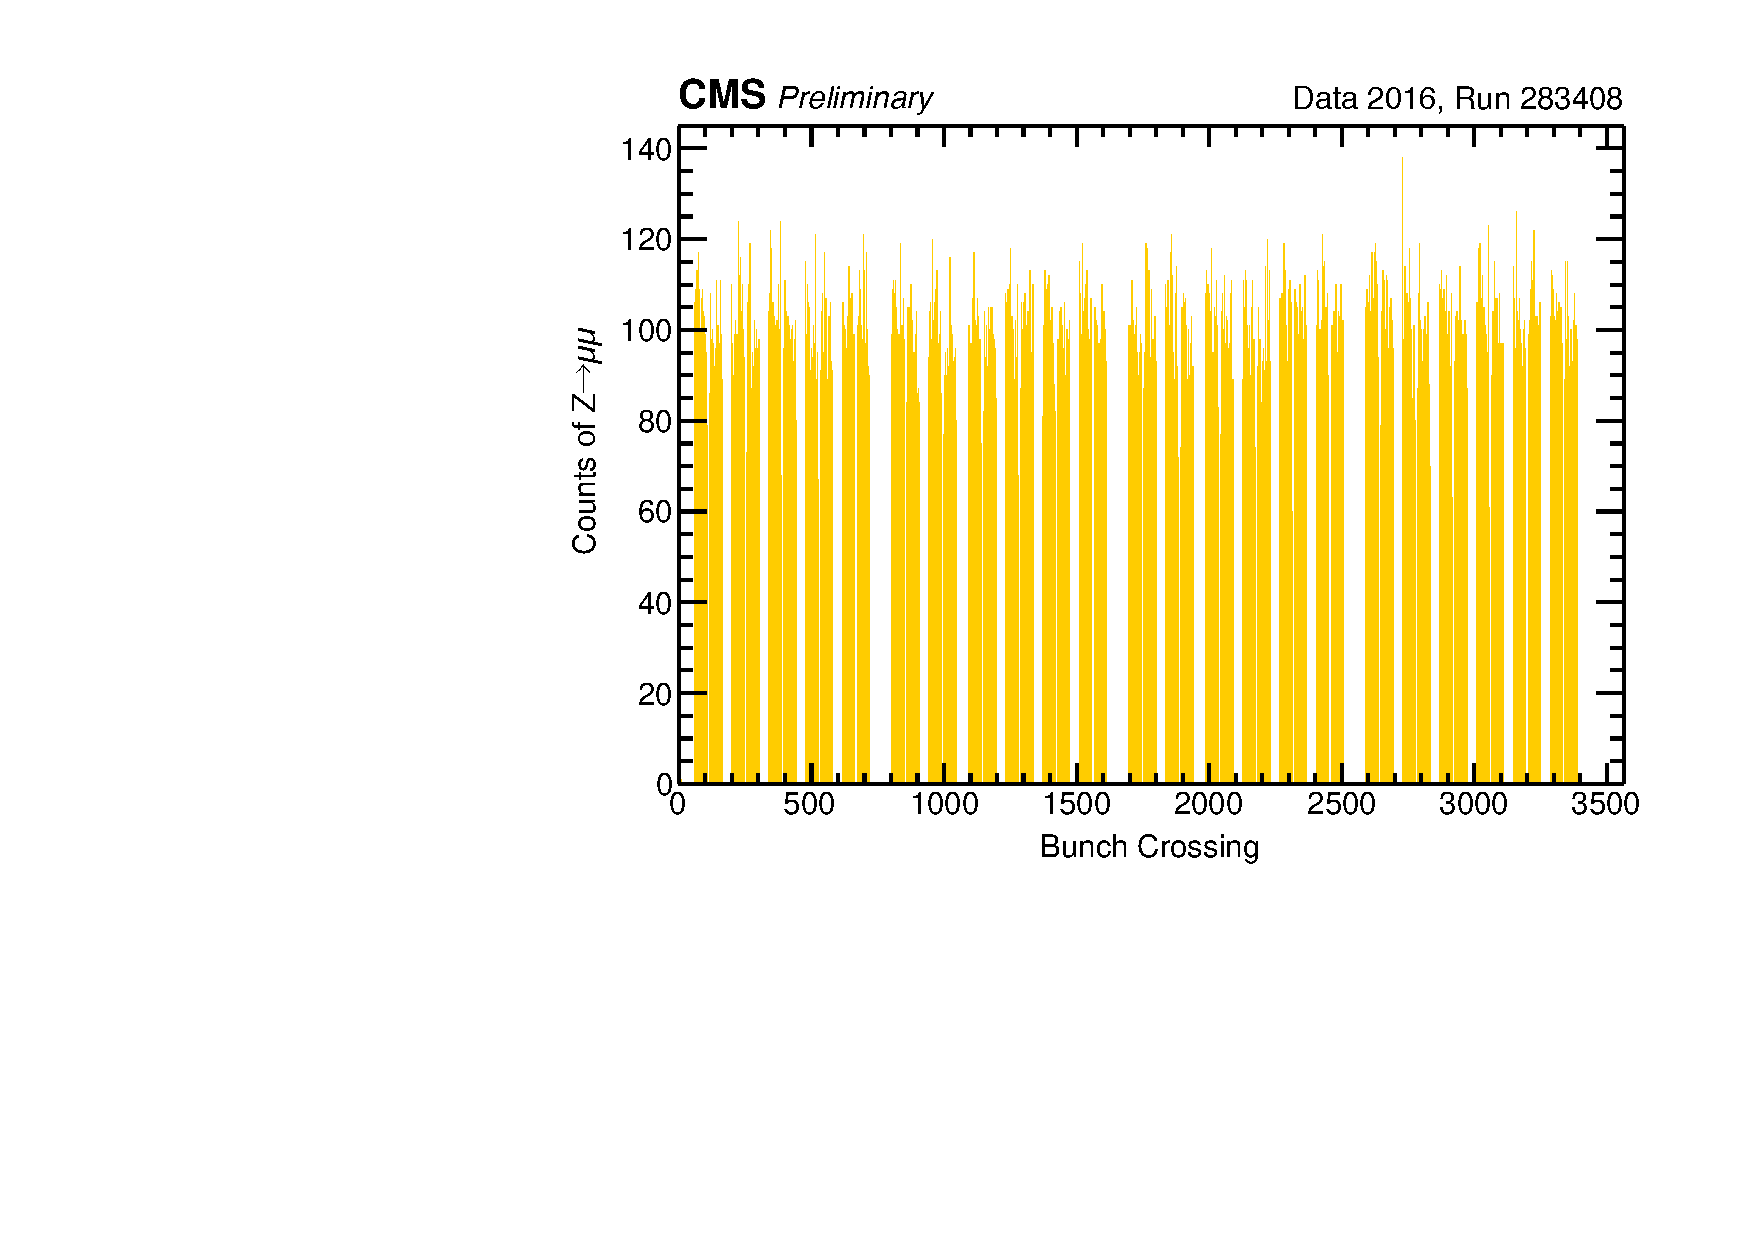
\includegraphics[width=\dummyFigWidth]{figures/neutron/BXstructure.pdf}
	\caption{Histogram of bunch crossing number in a particular CMS data taking period during LHC proton-proton collisions in 2016, showing the gaps of various sizes in the LHC bunch structure.}
	\label{fig:bunch_structure}
\end{figure}

The LHC proton beam has 3564 bunch places, with a bunch spacing of 25\unit{ns}. Not every bunch place has protons in it; rather, consecutive bunches of protons occur in trains, separated by gaps \cite{Evans:2008zzb}. Proton-proton collisions occur in CMS when bunches of protons cross, called bunch crossings (BX). \Fig~\ref{fig:bunch_structure} is a histogram of LHC bunch place numbers for a high statistics run. The non-empty histogram bins correspond to bunch places that are filled with \pp collisions, displaying the LHC bunch structure. In this run, trains with protons are exactly 48 bunches long and the trains are separated by bunch gaps of 8 to 35 bunch places, with the final train followed by the LHC abort gap of approximately 200 bunch places.

%In each event read out by the CMS DAQ, anode wire hits are read out from CSCs in 16 time bins of 25\unit{ns}. 
%As mentioned in \Sec~\ref{sec:csc_electronics}, hits in time with the muon occur in the middle of the readout window in time bin 8, so that time bins read out before time bin 8 correspond to earlier bunch places. Early-time hits found in events triggered by muons from \pp collisions in the first BX after a gap correspond to times within the gap, \ie during bunch places without any \pp collisions. Thus they must arise from \pp collisions before the gap (apart from the rare cosmic or noise hit), and we attribute them to neutron-induced hits from long-surviving neutrons, \ie neutron capture. Events with muons in time with the first few BX after a gap can also be used as long as the neutron-induced hits are early enough to fall within the gap. 

%Similarly, events with muons triggered just before the beginning of the gap have late-time hits that correspond to times in the gap. As the LHC bunch trains often have exactly 48 consecutive BX with collisions between gaps, for convenience we consider only trains of 48 BX that occur after gap of at least 35 bunch places.

In each event read out by the CMS DAQ, anode wire hits are read out in 16 time bins of 25 ns. As mentioned in \Sec~\ref{sec:csc_electronics}, hits in time with the muon occur in the middle of the readout window in time bin 8; time bins before time bin 8 then correspond to earlier bunch places. Hits from these early-time time bins where the readout was triggered by a muon from pp collisions in the first BX after a gap correspond to times within the gap. That is, these hits occur during bunch places without any pp collisions. Thus, they must arise from pp collisions from before the start of the gap (apart from the rare cosmic or noise hit), and we attribute them to be neutron-induced hits from long-surviving neutrons, i.e. from neutron capture. Events with muons that are triggered in the first few BXs after a gap can also be used to identify neutron-induced hits as long as the early-time time bins are early enough to occur within the gap. 

Similarly, events (triggered by muons) at the end of a bunch train have late-time time bins that correspond to times within the beginning of the next bunch gap. As the LHC bunch trains often have 48 consecutive BX with collisions between gaps, for convenience we consider only bunch trains that are exactly 48 BX long and that occur after gaps of at least 35 bunch places. 

\Fig~\ref{fig:rainbow} is a 2D histogram of the CSC anode wire hits (intensity given by color code) as a function of the number of bunch crossings after a gap on the $y$~axis and the digi readout time bin on the $x$~axis. Both BX and time bins are 25\unit{ns} wide. Time bin 8 is in-time with the muon that triggered readout of the chamber.

% Blotting out the appendices for now
%Appendix~\ref{sec:appendix_rainbow} contains similar plots for all chamber types, for both wire group hits and comparator half-strip hits.

The region bounded by the lower left red outlined triangle contains early readout time hits in early bunch places, \ie hits recorded near the end of an LHC bunch gap. This triangle contains neutron capture induced hits with negligible contribution from cosmic muons. The excess hits in readout time bin 0 contain hits from the previous bunch crossing due to the length of electronic pulses and are therefore not considered. We use the bins selected within the lower left triangle as the final step in isolating neutron capture induced hits. 

The central red outlined rectangle is a region delineating early readout time hits in bunch places contained completely within a bunch train. Hits from these bunch crossings consist of, in addition to neutron capture induced hits, hits induced by fast neutrons and hits in time with \pp collisions from other bunch crossings occurring in out-of-time readout time bins. The upper right red outlined triangle is a region delineating hits in late bunch places, \ie hits recorded at the beginning of an LHC bunch gap. Hits from these bunch crossings contain not only neutron capture induced hits, but also hits induced by fast neutrons (neutrons which have not yet lost enough energy to be captured) that occur within a few bunch crossings of a \pp collision. \Tab~\ref{tab:time_windows} summarizes the time windows for each of the three regions outlined in \FigDot~\ref{fig:rainbow}.

\begin{figure}[htbp]
	\centering
	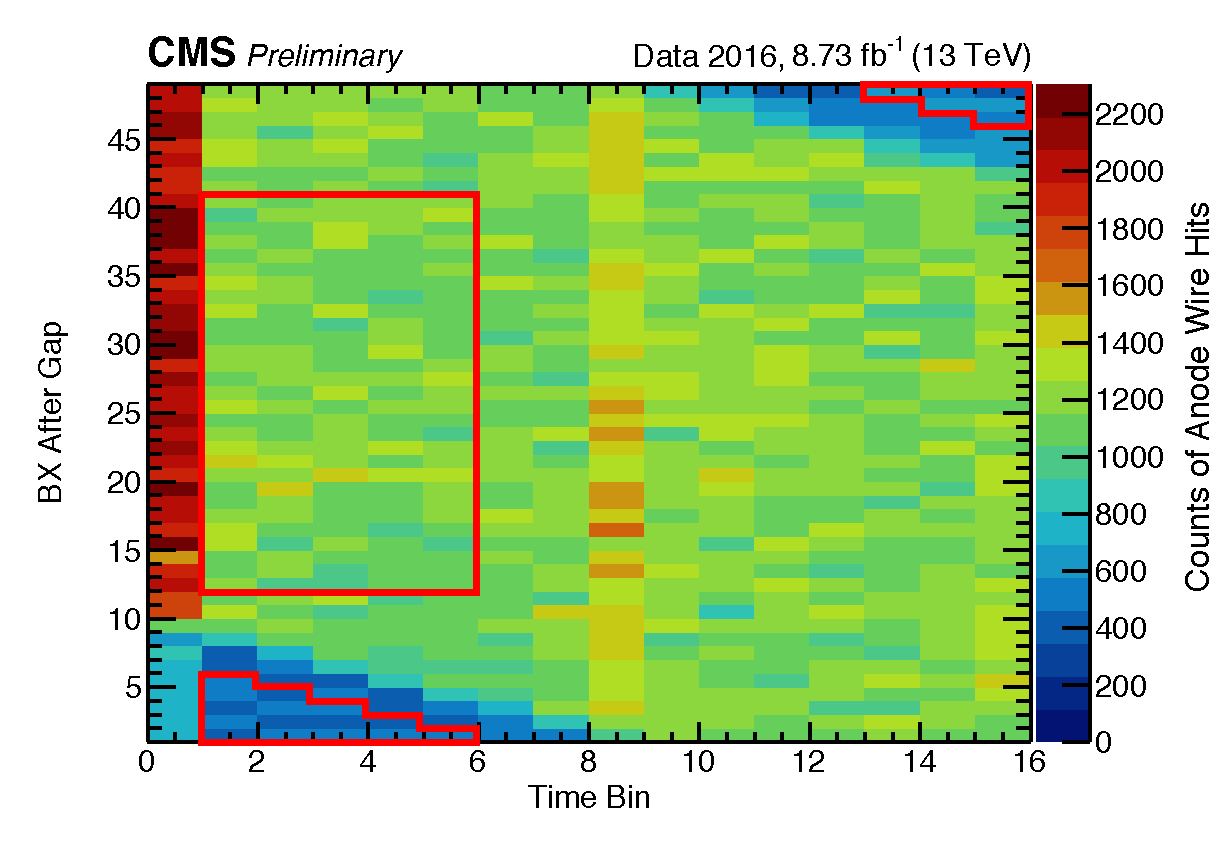
\includegraphics[width=\dummyFigWidth]{figures/neutron/Rainbow_wire_11.pdf}
  \caption[2D histogram of number of anode wire hits from CSCs in the inner ring of the first station (ME1/1) of the CMS endcap muon system.]{2D histogram of number of anode wire hits from CSCs in the inner ring of the first station (ME1/1) of the CMS endcap muon system. The histogram is plotted as a function of the readout time bin, and of number of bunch crossings (BX) after an LHC bunch gap of at least 35~BX in bunch trains that are exactly 48~BX in length. Hits in readout time bin 0 are contaminated with an artifact of anode wire readout electronics and are therefore not considered.}
	\label{fig:rainbow}
\end{figure}

\begin{table}
	\centering
  \topcaption[Enumeration of time windows used for each region listed by digi readout time bins and bunch places after the gap.]{Enumeration of time windows used for each region in \FigDot~\ref{fig:rainbow}, listed by digi readout time bins and bunch places after the gap.}
	\label{tab:time_windows}
	\begin{tabular}{p{200pt}lll}
		Region & BX After Gap ($b$) & Readout Time Bins ($T(b)$) & $N_{T(b)}$ \\ \hline \hline
		\multirow{5}{200pt}{Lower left triangle \newline (neutron capture only)}
			& 1 & 1--5 & 5      \\
			& 2 & 1--4 & 4      \\
			& 3 & 1--3 & 3      \\
			& 4 & 1--2 & 2      \\
			& 5 & 1    & 1      \\
		\textbf{Total 2D bins in region} & & & \textbf{15}\\[.5em] \hline
		\multirow{3}{200pt}{Central rectangle (neutron capture, fast neutrons, and hits from \pp collisions)}
			& 12--40 & 1--5 & 5     \\
			& & &                   \\
			& & &                   \\
		\textbf{Total 2D bins in region} & & & \textbf{145}\\[.5em] \hline
		\multirow{3}{200pt}{Upper right triangle \newline (neutron capture and fast neutrons)}
			& 46 & 15     & 1   \\
			& 47 & 14--15 & 2   \\
			& 48 & 13--15 & 3   \\
		\textbf{Total 2D bins in region} & & & \textbf{6}\\[.5em] \hline
	\end{tabular}
\end{table}

In summary, we select neutron capture induced hits in CMS data using the following criteria:
\begin{itemize}
	\item Triggering muons must be from \ZMM candidates in SingleMuon Run 2016H
	\item Exactly one LCT must be in a one-sixteenth corner of a chamber
	\item Digis must be in the opposite half of the chamber from the LCT
	\item Digis must be found at early times in events occurring in the first few bunch places in a train of size exactly 48 bunch places, after a bunch gap of at least 35 bunch places
\end{itemize}

\section{Results and Comparison of CMS Data with MC Simulation}
\label{sec:datamc}
\subsection{Computation of Neutron-Induced Hit Rates}
With the selection of neutron-induced hits in CMS data as well as the
understanding gained from neutron simulation at CMS, we examine the
local $r$ and $\phi$ distributions of neutron-induced hits within a
given chamber type, as well as the neutron-induced hit rate for a
given chamber as a function of instantaneous
luminosity \cite{Cousins:687399,CMS-PAS-LUM-17-001}. Directly
comparing CMS data and MC simulation requires careful normalization of
the digi counts. This section describes how the samples of
neutron-induced hits obtained using the procedures discussed in
\Sec~\ref{sec:selection} are normalized, and various
neutron-induced hit rates are defined.

As discussed in \Sec~\ref{sec:selection}, neutron captures
typically occur many bunch places after the \pp collisions that
created the neutrons, so that, to a good approximation,
neutron-induced hits uniformly populate all bunch places in the
LHC. Observation of early-time neutron-induced hits during a
particular triggering bunch crossing necessarily implies contributions
from many \pp collisions in many previous bunch crossings at CMS. In
the steady state of approximately constant instantaneous luminosity,
we can associate the aggregate number of all neutron-induced hits to
the aggregate number of all \pp collisions, even though the \pp
collisions are not uniformly spaced in time at CMS, having significant
gaps between bunch trains. This association is the basis for all our
rate calculations.
%Note from Bob: I decided that it was not a good idea to think about
%BX spatially ``around the ring'', but rather temporally at CMS

Since we connect rates of neutron-induced hits to approximately
constant instantaneous luminosity, it is convenient to use the
instantaneous luminosity as measured over a ``lumi section,'' a time
interval of data taking at CMS of about 23\unit{s}. We consider any
changes in instantaneous luminosity within a lumi section to be
negligible. We further consider edge effects from neutrons created
during one lumi section but detected during another to be negligible.
(The effects on the two ends of the a lumi section tend to cancel in
any case.)

As further discussed in \Sec~\ref{sec:selection}, the
neutron-induced hits that we observe are a random sample of the steady
stream of hits, where the number of samples varies from half-chamber
to half-chamber within CMS and with each event, according to the
selection criteria described. Thus, in order to normalize our
neutron-induced hit rates, we keep track of the number of times we
look for hits in each half chamber as well as the steady state rate
of \pp collisions at the times we look.

The bookkeeping accounts for each 2D bin in \FigDot~\ref{fig:rainbow},
each readout time bin and bunch place after the gap.  The details are
described in the next sections; here we define some variables to be
used.

Each ring specifies a different chamber type, represented by
$c$. These chamber types contain different numbers and sizes of wire
groups and half-strips; we let $d$ (for digi) represent a particular
wire group or half-strip within a given chamber type. The counts also
vary with the particular bunch place $b$ after a gap and the
particular readout time bin $\tau$ in which we look.

\subsubsection{Computation of Neutron Hit Rate in CMS Data}

To determine the neutron-induced hit rate in CMS data, we count the
number of selected digis found in particular bunch places after a gap
and particular time bins in one of the red outlined regions in
\FigDot~\ref{fig:rainbow}. These regions consist of a set $B$ of bunch
places after a gap, and a set $T(b)$ of time bins for each particular
bunch place $b\in B$ after a gap. \Tab~\ref{tab:time_windows}
enumerates each of the bunch places after a gap considered in each
region, consisting of a bunch place set $B$, the set of time bins
$T(b)$ for each bunch place, and the total number of time bins
$N_{T(b)}$ for each bunch place.  For all $b$ not in the table, $T(b)$
is the empty set.

We process our data as a series of DAQ events, as described in
\Sec~\ref{sec:selection}.  In the following, ``event'' refers to a
DAQ event, which corresponds to a trigger at a particular bunch
crossing leading to a complete readout of the detector. The event data
of course contains hits from many \pp collisions, including (in the
out-of-time time bins) hits from \pp collisions in other bunch
crossings.

We formalize our notation for counting the number of neutron-induced
digis in a somewhat tedious manner in order to help with the
bookkeeping that follows for keeping track of the associated \pp
collisions.

Let $N_\text{events}^\text{CMS}$ be the number of events in the data
set used; we let the index $i$ run over the events considered, so that
$i=1, \ldots, N^{\text{CMS}}_{\text{events}}$.

Let $b(i)$ be the number of the bunch place after a gap for event $i$.

Then $T(b(i))$ is the set of time bins examined in event $i$, either
the bins listed in \Tab~\ref{tab:time_windows} for the region under
study, or the empty set.  (For example, if the region under study is
the ``Lower left triangle'', then $T(b(i))$ is the empty set for $b(i)
> 5$.)

A chamber type $c$ represents multiple chambers in a ring; let $c_j$
represent the $j$th chamber in chamber type $c$, and let $N_c$
represent the total number of chambers of type $c$, so that
$j=1, \ldots, N_{c}$.


Let $I_\text{look}(i, c_j, d)$ denote an indicator function
representing whether or not we looked in wire group or half-strip $d$
of chamber $j$ of chamber type $c$ in event $i$.  That is,
$I_\text{look}(i, c_j, d)$ is 1 whenever $d$ is in a half chamber in
which we looked in event $i$, and 0 otherwise.

%hit counting begins here

Let $I_\text{hits}(i, c_j, d, \tau)$ denote an indicator function
representing whether or not a hit is present in time bin $\tau$ of
wire group or half-strip $d$ in chamber $j$ of chamber type $c$ in
event $i$.  That is, $I_\text{hits}(i, c_j, d, \tau)$ is 1 whenever a
hit is present, and 0 otherwise.

The product of the two indicator functions is 1 whenever we look for
hits and find them.  For each event $i$, we sum the product of the
indicator functions over the time bins examined for event $i$, then
over chambers of type $c$, and then further sum over events.

We thus obtain $N_\text{hits}^\text{CMS}(c, d)$, the number of digis
found in the data set in the examined time bins of chamber type $c$
and wire group or half-strip $d$:

\begin{equation}
	\label{eqn:indicator_nHits}
	N_\text{hits}^\text{CMS}(c, d) = 
        \sum_{i=1}^{N^\text{CMS}_\text{events}}
        \sum_{j=1}^{N_c} \ 
        \sum_{\tau\in T(b(i))}
        I_\text{look}(i, c_j, d) \times
        I_\text{hits}(i, c_j, d, \tau). 
\end{equation}

As is evident, this sums over all chambers of type $c$.  One may divide by
$N_c$ to get the average number of hits in one chamber of type $c$.

% pp collision computation begins here
%
We also formalize our notation for counting the number of $\pp$
collisions to be associated with the hits found.  This is complicated
by the varying luminosity (or equivalently, varying pileup and/or
fraction of LHC filled with bunches).

Given the association between the steady state number of \pp
collisions and the steady state number of hits, the number of \pp
collisions associated with event $i$ is given by the mean number
of \pp collisions during the time interval in which we look.  The time
interval in which we look in one time bin $\tau$ is the that of a time
bin in the CSC readout, namely 25 ns.  This is also the length in time
of a bunch place in the LHC.  Thus the associated number of \pp
collisions in event $i$ is given by the mean
number of \pp collisions \emph{per bunch place}, averaged over all
bunch places at CMS (including empty bunch places), when event $i$ was
acquired.
%Note from Bob: I decided that it was not a good idea to think about
%BX spatially ``around the ring'', but rather temporally at CMS
The latter is a product of two quantities: the mean number
of \pp collisions per {\em bunch crossing $P_i$} (also referred to as
pileup) for event $i$, as reported by the CMS BRIL group;
and the fraction of filled bunch places (bunch places that have bunch crossings),
which we call $f_\text{fill}$, and which is
approximately 0.62 for the data used in this analysis. 

We let $N^\text{CMS}_{\text{\pp}}(c, d)$ be
the total number of associated \pp collisions 
in the data set at wire group or half strip $d$ in chamber type
$c$. It is the number of associated \pp collisions, summed over all events:

\begin{equation}
        \label{eqn:nPP}	
	N^\text{CMS}_\text{\pp}(c, d) = 
        \sum_{i=1}^{N^\text{CMS}_\text{events}}
        \sum_{j=1}^{N_c} \ 
        \sum_{\tau\in T(b(i))}
        I_\text{look}(i, c_j, d) \times
        P_i \times f_\text{fill}
\end{equation}

As in \Eq~\ref{eqn:indicator_nHits},
this sums over all chambers of type $c$, and one may divide by
$N_c$ to get the average for one chamber of type $c$.

The sum over $\tau$ in \Eq~\ref{eqn:nPP} counts the same \pp
collisions more than once in an event $i$; this is because we may look
in more than one time bin, and the goal is to have a normalization for
each time bin, and hence for hits found.

%hits per pp begins here

Dividing \Eq~\ref{eqn:indicator_nHits} by \Eq~\ref{eqn:nPP}, we obtain
the number of hits per \pp collision {\em per wire group or
half-strip $d$} in chamber type $c$:

\begin{equation}
	\label{eqn:hits_perPP_perDigi}
\text{hits per \pp per $d$} = 
      \frac{N_\text{hits}^\text{CMS}(c,d)}{N_\text{\pp}^\text{CMS}(c,d)}.
\end{equation}

To convert \Eq~\ref{eqn:hits_perPP_perDigi} to a per area quantity, we divide by the area subtended by each wire group or half-strip $d$ in a chamber type $c$, denoted $A_\text{digi}(c, d)$. The neutron background hit rate per \pp collision per area at CMS is given by

\begin{equation}
	\label{eqn:hits_perA_perPP_perDigi}
\text{hits per \pp per area at $d$} = 
   \frac{1}{A_\text{digi}(c, d)}  \  \frac{N_\text{hits}^\text{CMS}(c,d)}{N_\text{\pp}^\text{CMS}(c,d)}
\end{equation}

The average neutron background hit rate per area for the entire chamber type $c$ is obtained by summing \Eq~\ref{eqn:hits_perPP_perDigi} over the set of possible wire groups and half-strips in a chamber type, denoted $D(c)$, and dividing by the chamber area $A_\text{CSC}(c)$:

\begin{equation}
	\label{eqn:hits_perA_perPP_perCSC}
\text{hits per \pp per area, avg.\ over $c$} = 
   \frac{1}{A_\text{CSC}(c)}  \  \sum_{d\in D(c)}{\frac{N_\text{hits}^\text{CMS}(c,d)}{N_\text{\pp}^\text{CMS}(c,d)}}
\end{equation}

To convert \Eqs~\ref{eqn:hits_perA_perPP_perDigi} and \ref{eqn:hits_perA_perPP_perCSC} to per time quantities, we choose a reference luminosity $\pazocal{L}_0$ and multiply by the mean \pp collision rate per time at that luminosity, $N_\text{\pp}^\text{CMS}/t$. That is,

\begin{equation}
    \label{eqn:hits_perA_perT_perDigi}
\text{hits per \pp per area per time at $d$} =  
  \frac{1}{A_\text{digi}(c, d)}  \  \frac{N_\text{hits}^\text{CMS}(c,d)}{N_\text{\pp}^\text{CMS}(c,d)}  \  \left.\frac{N_\text{\pp}^\text{CMS}}{t}\right|_{\pazocal{L}_0}
\end{equation}

and similarly for the number of hits in the entire chamber,

\begin{equation}
    \label{eqn:hits_perA_perT_perCSC}
\text{hits per \pp per area per time, avg.\ over $c$} =   
  \frac{1}{A_\text{CSC}(c)}  \  \sum_{d\in D(c)}{\frac{N_\text{hits}^\text{CMS}(c,d)}{N_\text{\pp}^\text{CMS}(c,d)}} \  \left.\frac{N_\text{\pp}^\text{CMS}}{t}\right|_{\pazocal{L}_0}
\end{equation}

We obtain the mean \pp collision rate, $N_\text{\pp}^\text{CMS}/t$,
via two related methods. In the first method, we multiply the 
measured \pp interaction cross section and the
instantaneous luminosity:

\begin{equation}
    \label{eqn:sigmaPP_x_lumi}
    \left.\frac{N_\text{\pp}^\text{CMS}}{t}\right|_{\pazocal{L}_0} = \sigma_\text{\pp}  \  \pazocal{L}_0
\end{equation}

In  the second method, we multiply the mean pileup $P_0$ at a reference luminosity $\pazocal{L}_0$ by the fill fraction $f_\text{fill}$, and divide by 25\unit{ns}, the bunch spacing interval. 

\begin{equation}
    \label{eqn:PU_x_ff_over_BS}
	\left.\frac{N_\text{\pp}^\text{CMS}}{t}\right|_{\pazocal{L}_0} = \frac{f_\text{fill}  \  P_0}{25\unit{ns}}  \  \frac{10^9\unit{ns}}{\text{s}}.
\end{equation}

Both methods for measuring $N_\text{\pp}^\text{CMS}/t$ should give the same answer if we use the same cross section
as used by the CMS BRIL group when computing pileup numbers \cite{Sirunyan:2018nqx,PileupTwiki}.
We favor the second method of computing $N_\text{\pp}^\text{CMS}/t$ because it uses only quantities which are directly provided by the CMS BRIL group. 

In either case, the \pp collision rate can in principle be scaled to other luminosities:

\begin{equation}
    \label{eqn:PU_x_ff_over_BS_scale}
	\left.\frac{N_\text{\pp}^\text{CMS}}{t}\right|_{\pazocal{L}} = 
	\left.\frac{N_\text{\pp}^\text{CMS}}{t}\right|_{\pazocal{L}_0}  \  \frac{\pazocal{L}}{\pazocal{L}_0}.
\end{equation}
Consistency checks are shown in \FigsDot~\ref{fig:dppdt_vs_L} and \ref{fig:lumi_vs_pu}.

\Fig~\ref{fig:dppdt_vs_L} is a plot of the measured $N_\text{\pp}^\text{CMS}/t$ \vs instantaneous luminosity via the second method described above. In the plot, each black dot in the plot represents a single luminosity section and the slope of this line corresponds to the \pp interaction cross section, $\sigma_\text{\pp}$. From \FigDot~\ref{fig:dppdt_vs_L} we read off the \pp collision rate at any instantaneous luminosity. At the reference luminosity \reflumi, $N_\text{\pp}^\text{CMS}/t \approx 7\times10^8 \unit{\text{\pp}/s}$.  

\Fig~\ref{fig:lumi_vs_pu} shows a plot of instantaneous luminosity \vs mean pileup. Each dot in the plot represents a single luminosity section and is color coded according to the $f_\text{fill}$ for that data taking period. Approximately 95\% of the data collected corresponds to $f_\text{fill} = 0.62$. As a check that the two methods for calculating $N_\text{\pp}^\text{CMS}/t$ are equivalent, lines are drawn according to the $f_\text{fill}$ of various data taking conditions and the measured \pp interaction cross section \cite{Bawej:1711011, Sirunyan:2018nqx}. 

\begin{figure}
	\centering
	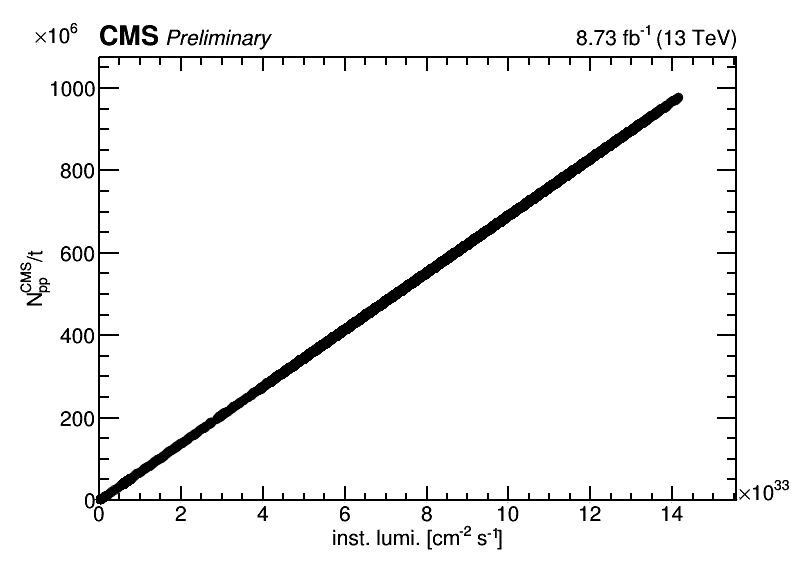
\includegraphics[width=\dummyFigWidth]{figures/neutron/dppdt_vs_L.png}
  \caption[Plot of $N_\text{\pp}^\text{CMS}/t$ \vs instantaneous luminosity.]{Plot of $N_\text{\pp}^\text{CMS}/t$ \vs instantaneous luminosity. Each dot denotes single luminosity section.}
	\label{fig:dppdt_vs_L}
\end{figure}

\begin{figure}
	\centering
	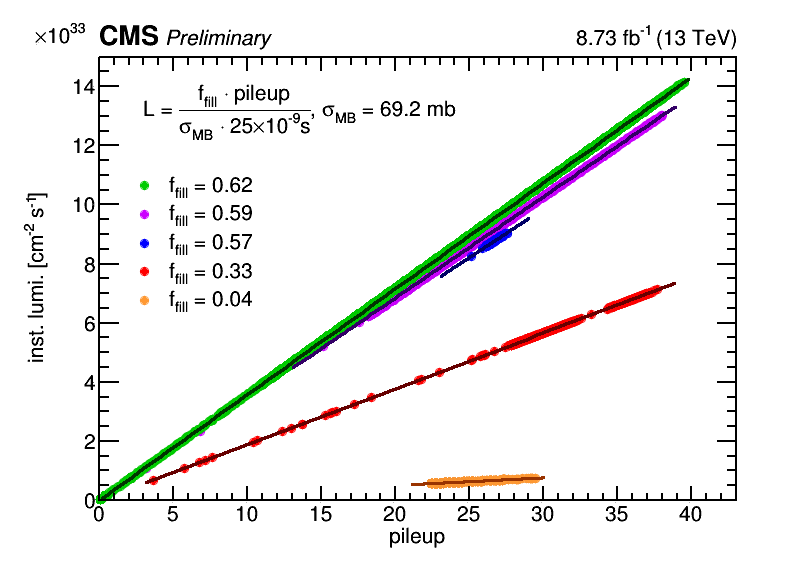
\includegraphics[width=\dummyFigWidth]{figures/neutron/lumi_vs_pu_allfills.png}
  \caption[Plot of instantaneous luminosity \vs mean pileup.]{Plot of instantaneous luminosity \vs mean pileup. Each dot denotes single luminosity section and the color denotes the fraction of filled bunches, $f_\text{fill}$, during which that data were collected.}
	\label{fig:lumi_vs_pu}
\end{figure}

\subsubsection{Computation of Neutron Hit Rate in CMS as a Function of Luminosity}
\label{sec:hit_rate_vs_lumi}

The above hit rates per \pp collision are independent of luminosity, and the per time rates are with respect to a reference luminosity. In this section we check the implicit assumption of linearity of rates with luminosity. We count the number of neutron hits, binned by the luminosity of the event in which the muon that generated the trigger occurred, and normalize to the number of times we look, binned by luminosity. 

At the risk of confusion, we let $\pazocal{L}$ refer to a luminosity {\em bin} centered on $\pazocal{L}$ , and let $I_\text{lumi}(i, \pazocal{L})$ denote an indicator function representing whether or not event $i$ occurred with a luminosity within luminosity bin $\pazocal{L}$. Then the computation of hit rates within
luminosity bins is the same as in \Eq~\ref{eqn:indicator_nHits}, 
with the addition of an indicator function to specify the luminosity bin.

We thus obtain $N_\text{hits}^\text{CMS}(c, d, \pazocal{L})$
the number of digis found in the data set in the examined time bins of
chamber type $c$ and wire group or half-strip $d$, in luminosity bin $\pazocal{L}$:

\begin{equation}
 	\label{eqn:nHits_Lumi}
        N_\text{hits}^\text{CMS}(c, d, \pazocal{L}) = 
        \sum_{i=1}^{N^\text{CMS}_\text{events}}
        \sum_{j=1}^{N_c} \ 
        \sum_{\tau\in T(b(i))}
        I_\text{look}(i, c_j, d) \times
        I_\text{hits}(i, c_j, d, \tau) \times
        I_\text{lumi}(i, \pazocal{L}). 
\end{equation}

The normalization for each luminosity bin, $N^\text{CMS}_\text{looks}(c,
d, \pazocal{L})$, is the sum of the number of times we looked in the
luminosity bin as in \Eq~\ref{eqn:nPP}, without the factors counting \pp
collisions:

\begin{equation}
 	\label{eqn:nLooks_Lumi}        
        N^\text{CMS}_\text{looks}(c, d, \pazocal{L}) = 
        \sum_{i=1}^{N^\text{CMS}_\text{events}}
        \sum_{j=1}^{N_c} \ 
        \sum_{\tau\in T(b(i))}
        I_\text{look}(i, c_j, d) \times
        I_\text{lumi}(i, \pazocal{L}).
\end{equation}

Then we can define rates similar to those defined in \Eqs~\ref{eqn:hits_perPP_perDigi}--\ref{eqn:hits_perA_perPP_perCSC} that are functions of luminosity:

\begin{equation}
	\label{eqn:hits_perLook_perDigi_Lumi}
\text{normalized hits per $d$} = 
   \frac{{N}^\text{CMS}_\text{hits}}{N^\text{CMS}_{\text{looks}}}(c, d, \pazocal{L})
\end{equation}
\begin{equation}
    \label{eqn:hits_perA_perLook_perDigi_Lumi}
\text{normalized hits per area at $d$} = 
  \frac{1}{A_\text{digi}(c, d)}  \  \frac{{N}^\text{CMS}_\text{hits}}{N^\text{CMS}_{\text{looks}}}(c, d, \pazocal{L})
\end{equation}
\begin{equation}
    \label{eqn:hits_perA_perLook_perCSC_Lumi}
\text{normalized hits per area, avg.\ over $c$} = 
  \frac{1}{A_\text{CSC}(c)}  \  \sum_{d\in D(c)}{\frac{{N}^\text{CMS}_\text{hits}}{N^\text{CMS}_{\text{looks}}}(c, d, \pazocal{L})}
\end{equation}

To convert \Eqs~\ref{eqn:hits_perA_perLook_perDigi_Lumi} and \ref{eqn:hits_perA_perLook_perCSC_Lumi} to per time quantities, we observe that each time we look corresponds to a 25~ns time interval readout time bin, and also one bunch space. Therefore, the neutron hit rate in chamber type $c$ as a function of luminosity is simply \Eq~\ref{eqn:hits_perA_perLook_perCSC_Lumi} multiplied by the conversion from time bin to ns:

\begin{equation}
    \label{eqn:hits_perA_perT_perCSC_Lumi}
\text{normalized hits per area per time, avg.\ over $c$} = 
    \frac{1}{A_\text{CSC}(c)}  \  \sum_{d\in D(c)}{\frac{{N}^\text{CMS}_\text{hits}}{N^\text{CMS}_{\text{looks}}}(c, d, \pazocal{L})}  \  \frac{\text{time bin}}{25\unit{ns}}  \  \frac{10^9\unit{ns}}{\unit{s}}
\end{equation}

\subsubsection{Computation of Neutron Hit Rate in MC Simulation}

In MC simulation, we identify the neutron capture induced hits in each
simulated event by the long time that is recorded since the pp
collision of the event.  In the rest of this section, when we refer to
hits or digis, we refer to those with late enough times to be
identified as being induced by neutron capture.

There is no need for a selection process as described for the CMS
data (with LCTs in a corner, etc).  All digis in all chambers in all
simulated events are examined.  We again invoke the approximation
described in \Sec~\ref{sec:datamc} that we can associate the aggregate
number of all neutron-induced hits to the aggregate number of all \pp
collisions, even though the \pp collisions are not uniformly spaced in
time at CMS.  Thus we need not be concerned with recording the
hit-by-hit time bin of simulated hits, but rather work with totals and
averages.


At CMS, this steady-state number of neutron-induced hits per \pp
collision at CMS, measured in one time bin (25\unit{ns}), is the sum
of hits induced by neutrons originating from all previous pp
collisions. A key point is that it is not necessary to attempt such a
sum, which would be awkward computationally.  Rather, we note that
this sum is equal to the sum of all simulated neutron-induced hits
(in all future time bins) coming from a single simulated pp collision.


Let $N_\text{events}^\text{MC}$ be the number of simulated events
considered.

Let $N_\text{hits}^\text{MC}(c, d)$ be the total number of hits in
$N^\text{MC}_\text{events}$ at wire group or half-strip $d$ (for digi)
in chamber type $c$. In analogy with \Eq~\ref{eqn:indicator_nHits}, we
can write, using all hits in all times,

\begin{equation}
	\label{eqn:MC_nHits}
	N_\text{hits}^\text{MC}(c, d) = 
        \sum_{i=1}^{N^\text{MC}_\text{events}}
        \sum_{j=1}^{N_c} \ 
        \sum_{\text{all~}\tau}
        \ 1
\end{equation}

As with data, this sums over all chambers of type $c$.  One may divide
by $N_c$ to get the average number of hits in one chamber of type $c$.

We let $N_\text{\pp}^\text{MC}(c)$ be the normalization to \pp
collisions for this hit total. (We suppress the argument $d$ since
unlike data, all wire groups and half strips are examined in every
event.)  While one MC event corresponds to a single simulated \pp
collision, the sum over $N_c$ chambers in \Eq~\ref{eqn:MC_nHits} means
that a factor of $N_c$ is needed to consistently normalize, i.e.,

\begin{equation}
    N_\text{\pp}^\text{MC}(c) = N_\text{events}^\text{MC}  \  N_c
\end{equation}

Then the number of hits per \pp collision at $d$ is then

\begin{equation}
    \label{eqn:MC_hits_perPP_perDigi}
 \text{hits per \pp per $d$, MC} = 
    \frac{N_\text{hits}^\text{MC}(c,d)}{N_\text{\pp}^\text{MC}(c)}
\end{equation}

As in data, we convert $N_\text{hits}^\text{MC}(c, d)/N_\text{\pp}^\text{MC}(c)$ to a per area quantity by dividing by $A_\text{digi}(c, d)$. The neutron hit rate per \pp collision in MC simulation is thus given by:

\begin{equation}
	\label{eqn:MC_hits_perA_perPP_perDigi}
\text{hits per \pp per area at $d$, MC} = 
	\frac{1}{A_\text{digi}(c, d)}  \  \frac{N_\text{hits}^\text{MC}(c, d)}{N_\text{\pp}^\text{MC}(c)}
\end{equation}

and similarly for the number of simulated hits in the entire chamber,

\begin{equation}
	\label{eqn:MC_hits_perA_perPP_perCSC}
\text{hits per \pp per area, avg.\ over $c$, MC} = 
	\frac{1}{A_\text{CSC}(c)}  \  \frac{1}{N_\text{\pp}^\text{MC}(c)}  \  \sum_{d\in D(c)}{N_\text{hits}^\text{MC}(c, d)}
\end{equation}

Finally, we convert \Eq~\ref{eqn:MC_hits_perA_perPP_perDigi} and \ref{eqn:MC_hits_perA_perPP_perCSC} to per time quantities by choosing a reference luminosity $\pazocal{L}_0$ and multiplying by the \pp collision rate per time at that luminosity, $N_\text{\pp}^\text{MC}/t$:

\begin{equation}
	\label{eqn:MC_hits_perA_perT_perDigi}
\text{hits per \pp per area per time at $d$, MC} = 	\frac{1}{A_\text{digi}(c, d)}  \  \frac{N_\text{hits}^\text{MC}(c, d)}{N_\text{\pp}^\text{MC}(c)}  \  \frac{N_\text{\pp}^\text{MC}}{t} 
\end{equation}

and 

\begin{equation}
	\label{eqn:MC_hits_perA_perT_perCSC}
\text{hits per \pp per area per time, avg.\ over $c$, MC} = 
    \frac{1}{A_\text{CSC}(c)}  \  \frac{1}{N_\text{\pp}^\text{MC}(c)}  \  \sum_{d\in D(c)}{N_\text{hits}^\text{MC}(c, d)}  \  \frac{N_\text{\pp}^\text{MC}}{t} 
\end{equation}
 
\subsection{Results}
\begin{figure}[htbp]
	\centering
	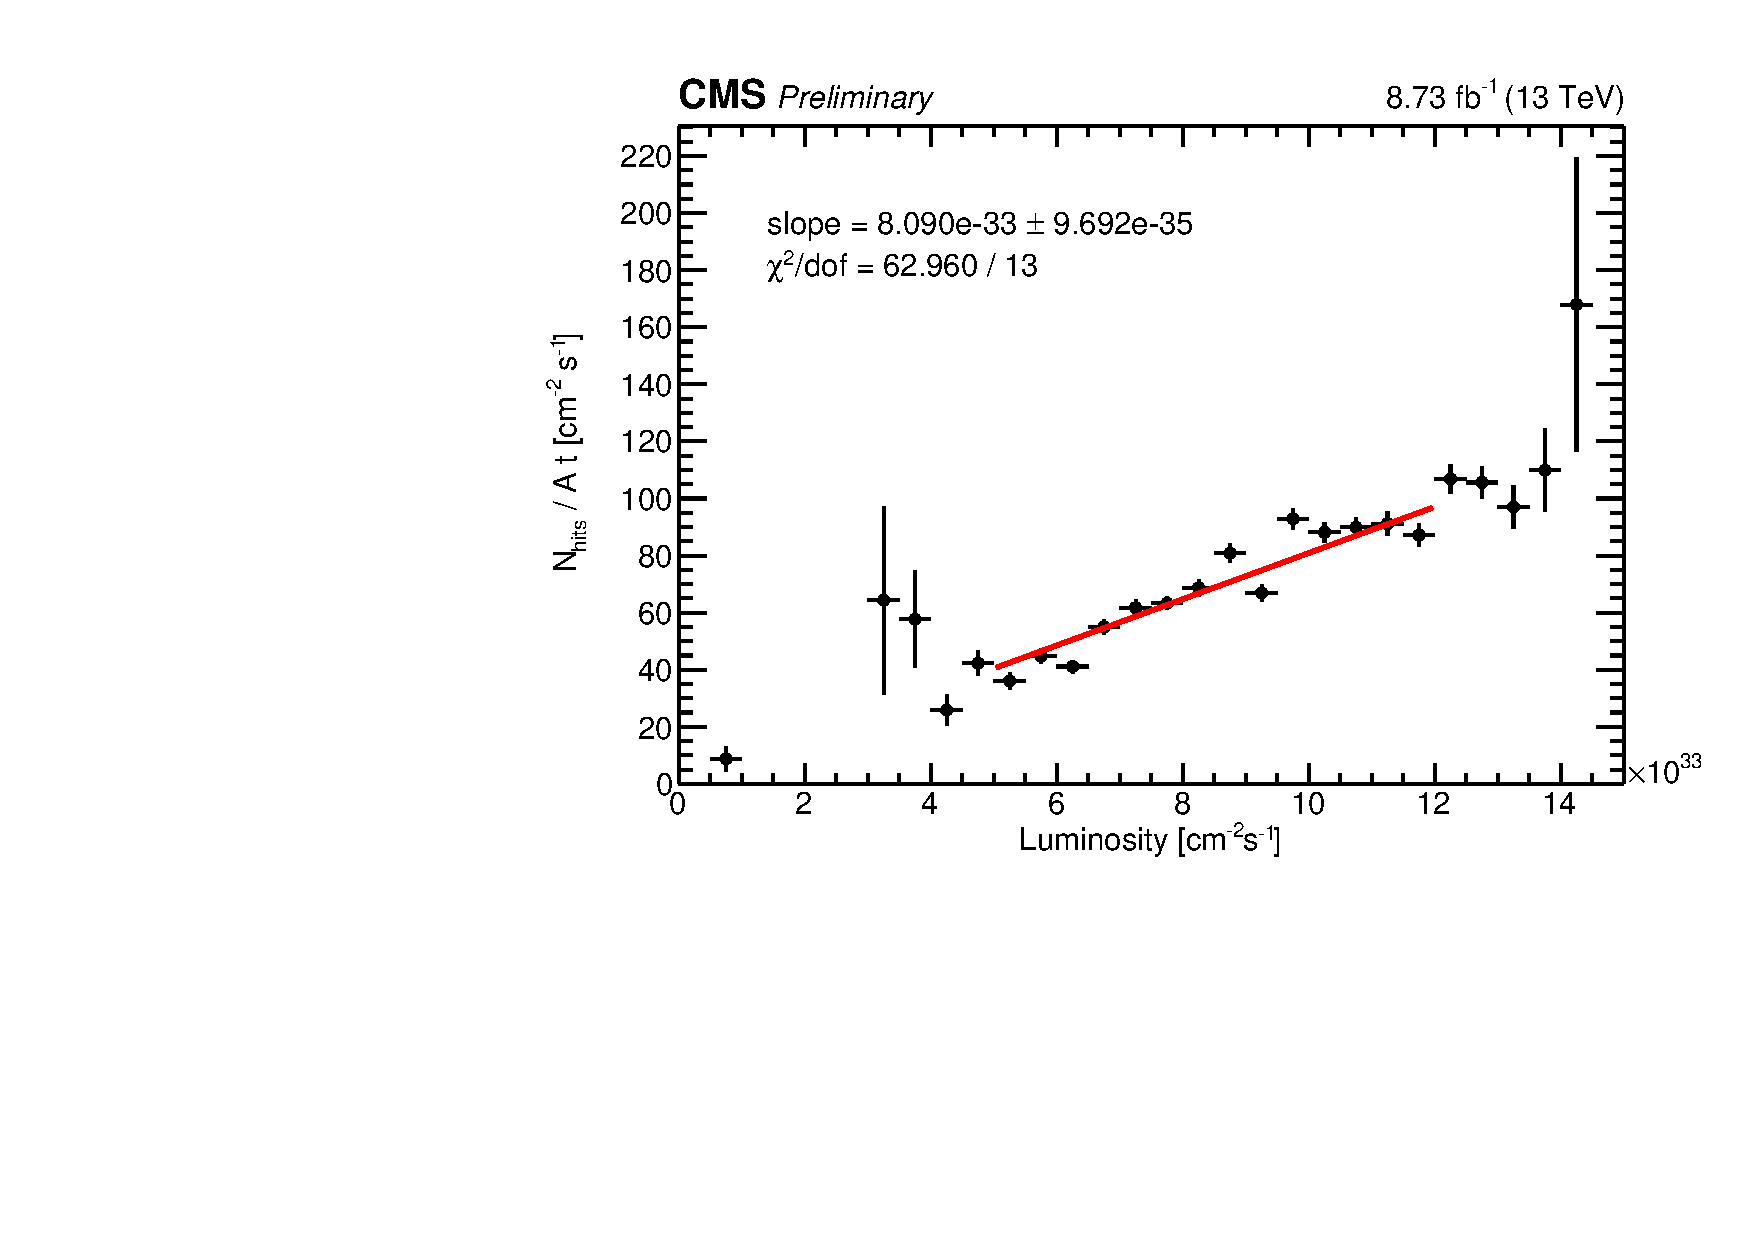
\includegraphics[width=0.85\dummyFigWidth]{figures/neutron/luminosity_11_wire_early_AREA_TIME_LOOK_20180628_fit.pdf}
	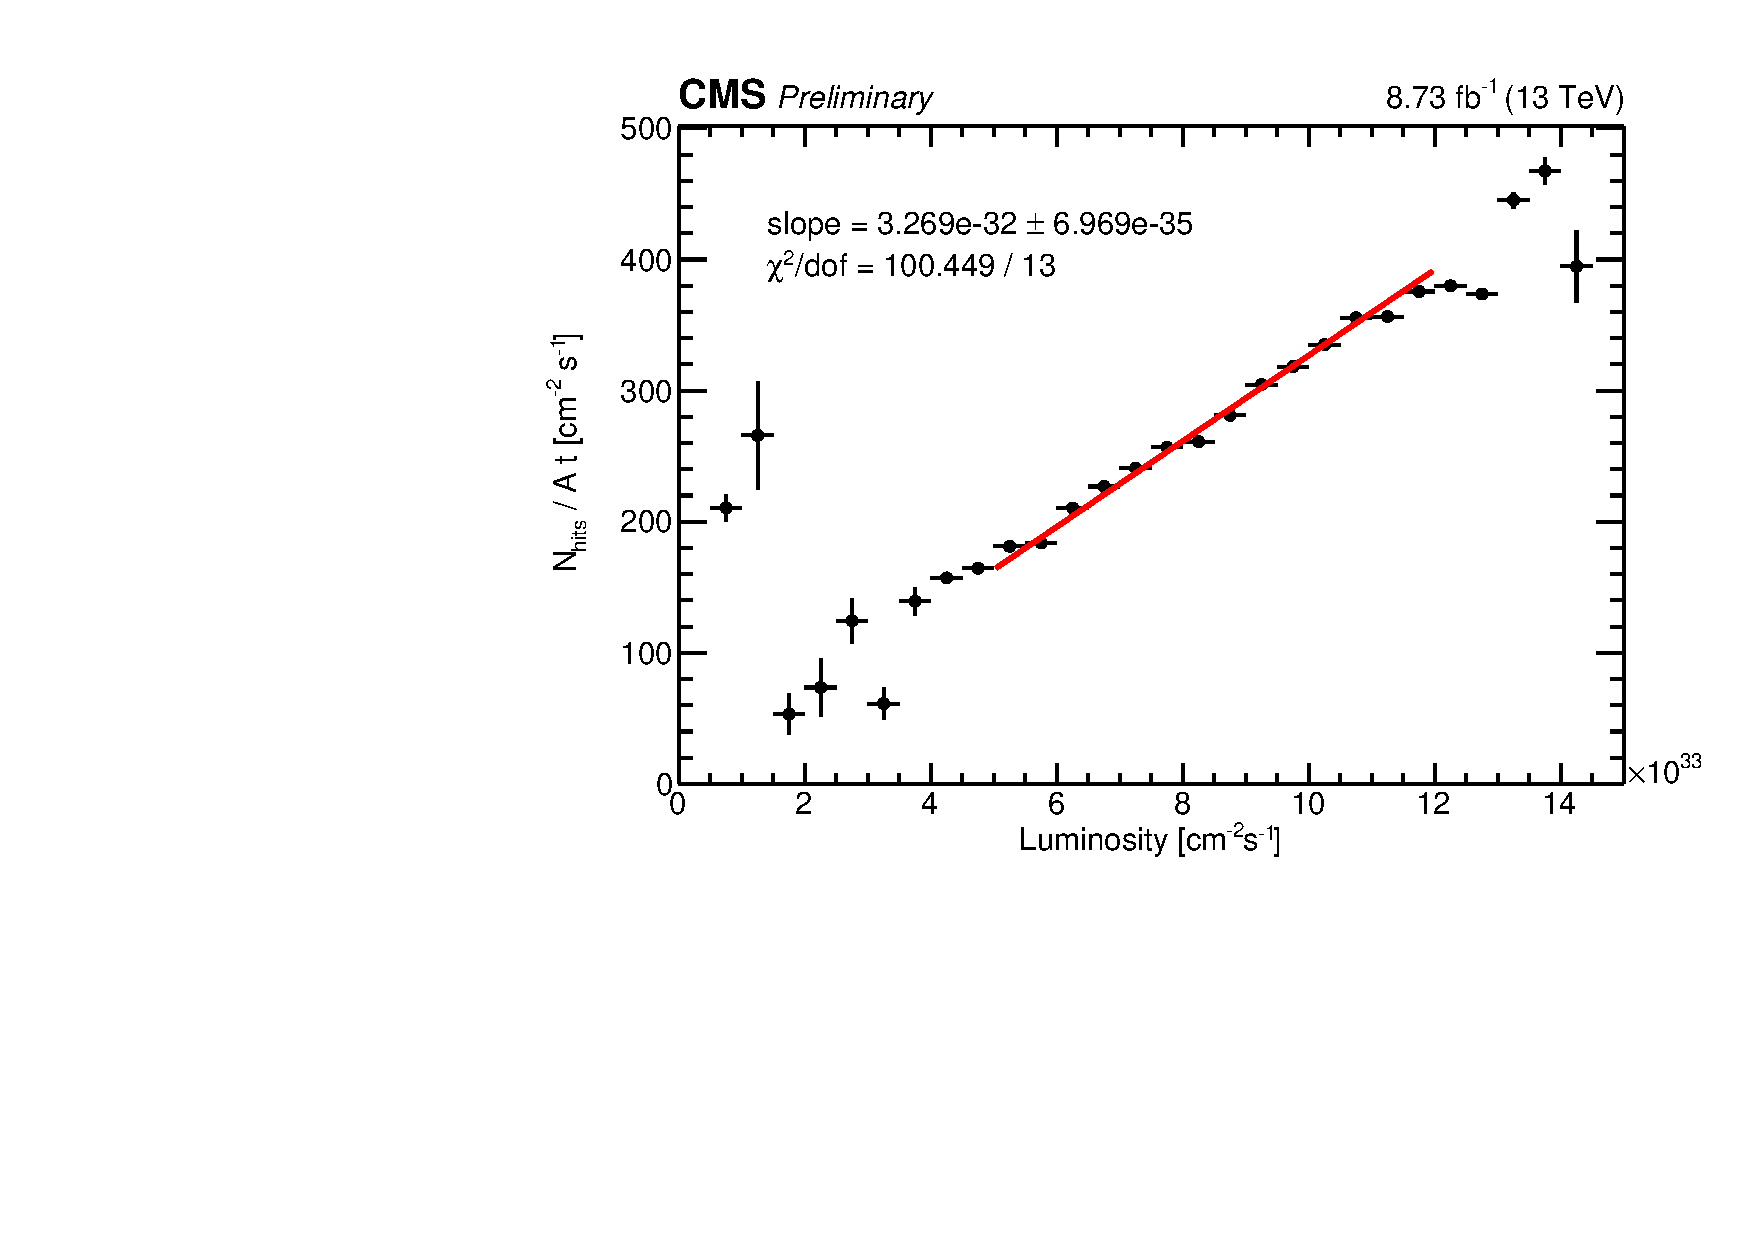
\includegraphics[width=0.85\dummyFigWidth]{figures/neutron/luminosity_11_wire_total_AREA_TIME_LOOK_20180628_fit.pdf}
  \caption[Plot of hits per time per area as a function of luminosity for ME1/1 chambers.]{Plot of hits per time per area as a function of luminosity as calculated in \Eq~\ref{eqn:hits_perA_perT_perCSC_Lumi} for ME1/1 chambers, (\posstyle{top}) for hits that occur at the end of LHC gaps (candidate neutron capture induced hits) and (\posstyle{bottom}) for hits that occur during \pp collisions. The red line is a linear fit constrained to go through the origin and fit over the central region of luminosity.}
	\label{fig:lumi_11}
\end{figure}
\begin{figure}[htbp]
	\centering
	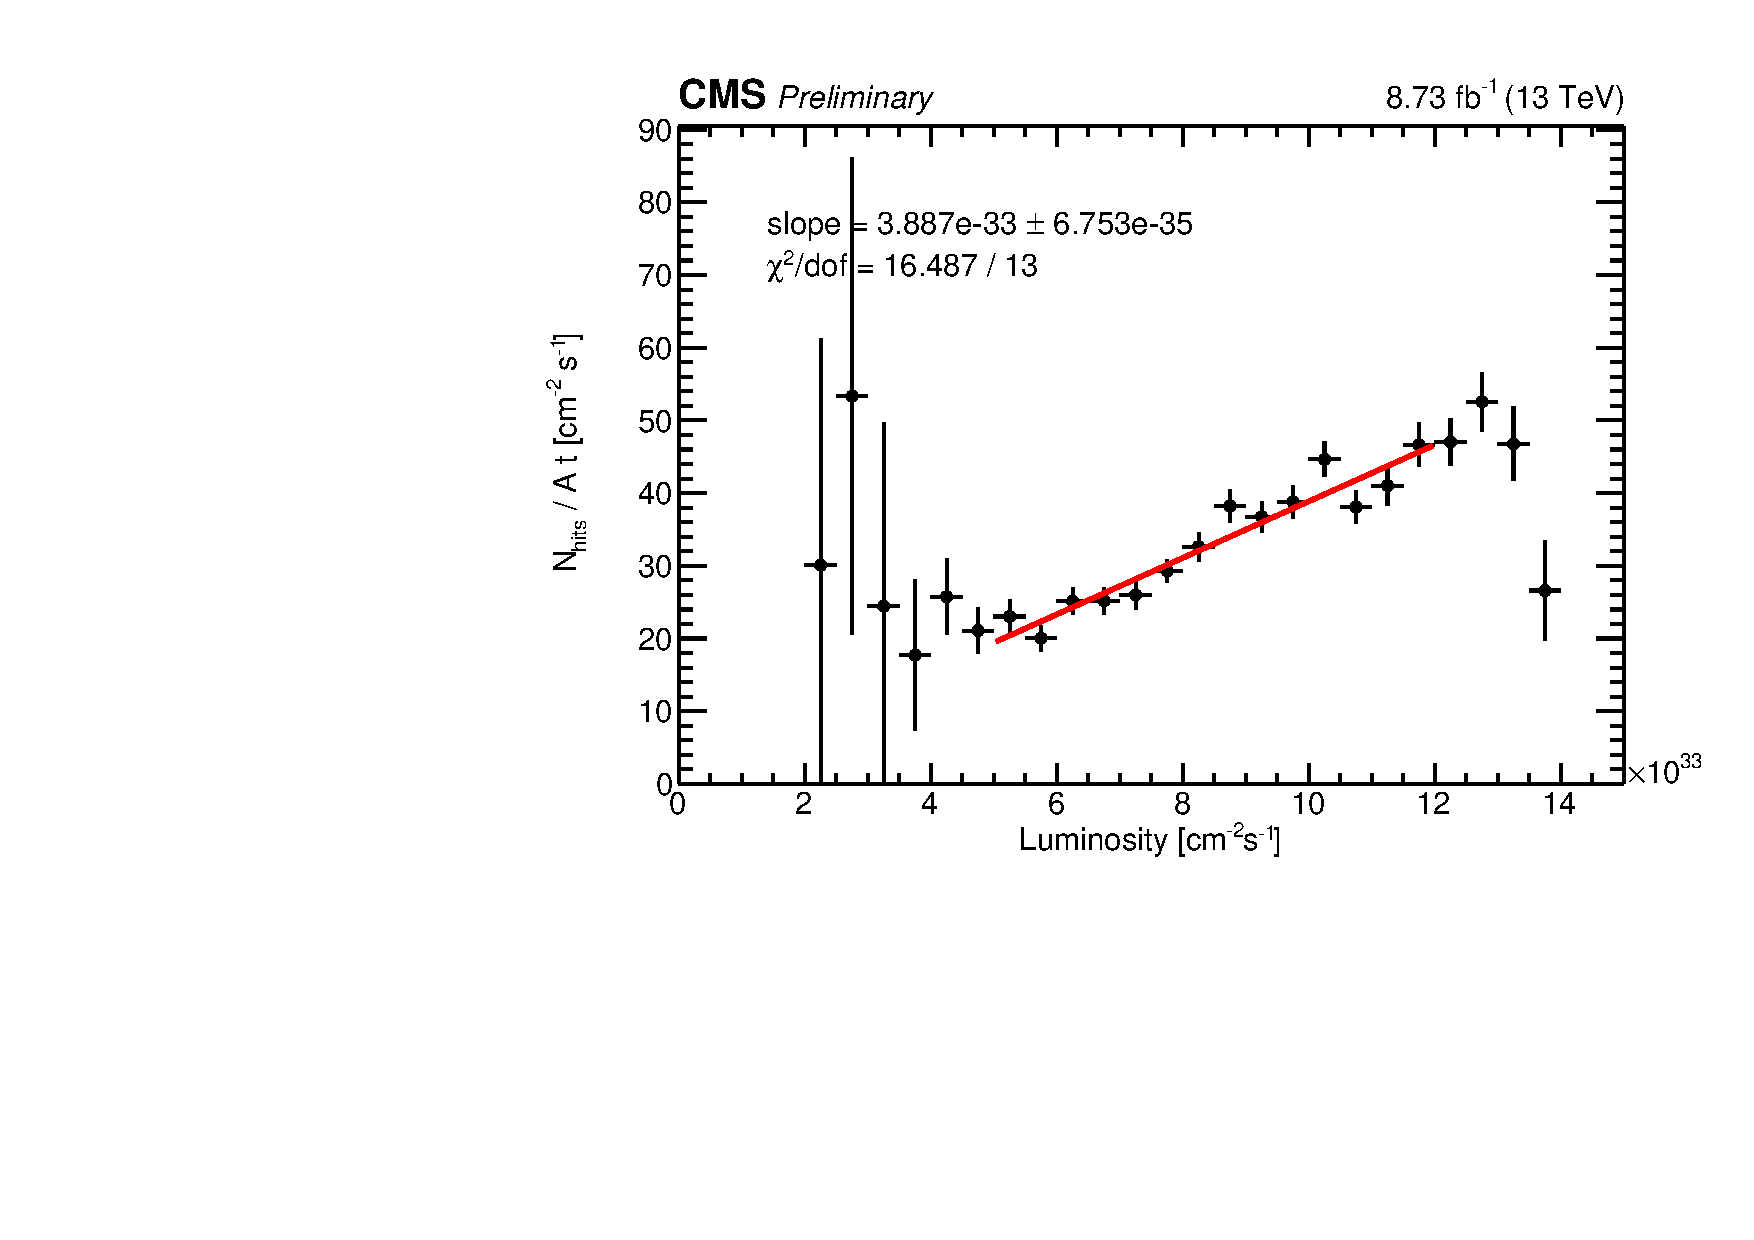
\includegraphics[width=0.85\dummyFigWidth]{figures/neutron/luminosity_21_wire_early_AREA_TIME_LOOK_20180628_fit.pdf}
	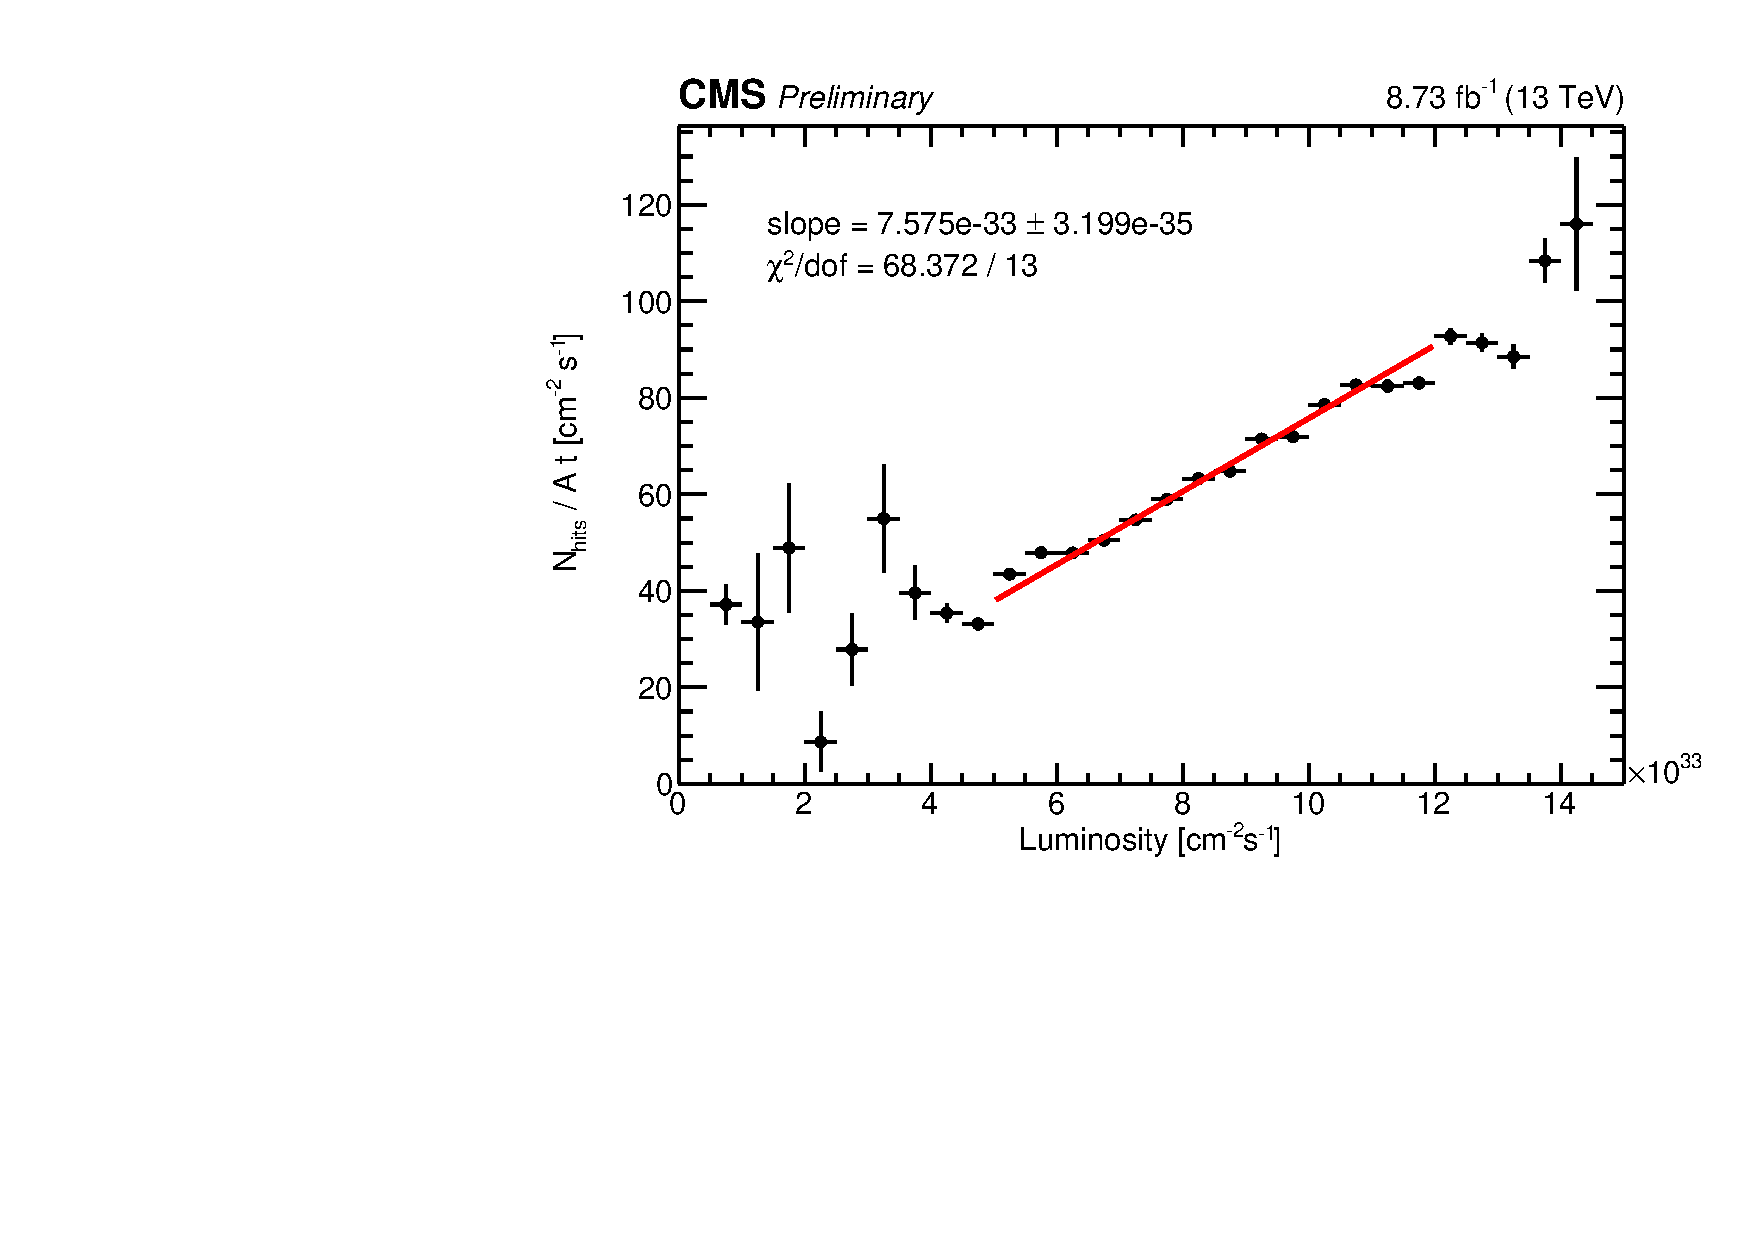
\includegraphics[width=0.85\dummyFigWidth]{figures/neutron/luminosity_21_wire_total_AREA_TIME_LOOK_20180628_fit.pdf}
  \caption[Plot of hits per time per area as a function of luminosity for ME2/1 chambers.]{Plot of hits per time per area as a function of luminosity as calculated in \Eq~\ref{eqn:hits_perA_perT_perCSC_Lumi} for ME2/1 chambers, (\posstyle{top}) for hits that occur at the end of LHC gaps (candidate neutron capture induced hits) and (\posstyle{bottom}) for hits that occur during \pp collisions. The red line is a linear fit constrained to go through the origin and fit over the central region of luminosity.}
	\label{fig:lumi_21}
\end{figure}

\Figs~\ref{fig:lumi_11} and \ref{fig:lumi_21} display plots of neutron-induced wire group hit rate without normalizing to \pp collisions (as in \Eq~\ref{eqn:hits_perA_perT_perCSC_Lumi}) \vs luminosity, for hits that occur at the end of LHC bunch gaps (lower left triangle from \FigDot~\ref{fig:rainbow}) and hits that occur during CMS \pp collisions (rectangle in \FigDot~\ref{fig:rainbow}), for ME1/1 and ME2/1 chambers, respectively. We plot the hit rate that is not normalized to \pp collisions, a quantity that is a function of luminosity, in order to see any potential linear dependence of hits \vs luminosity. Indeed, these plots show a relationship that is linear to the eye and intercepts the origin. This suggests that we have succeeded in isolating neutron capture induced hits, because contamination from muon-induced background would result in a positive offset on the $y$~axis. Fluctuations in the data points are presumably due to changes in data taking conditions; however, the size of the $\chi^2$/dof from the fit suggest that there are some systematic uncertainties that are not understood. 

\Figs~\ref{fig:wg_occupancy_11} and \ref{fig:wg_occupancy_21} display histograms of the neutron-induced wire group hit rate for CMS data and MC, \Eqs~\ref{eqn:hits_perA_perT_perDigi} and \ref{eqn:MC_hits_perA_perT_perDigi}, as a function of wire group number, in ME1/1 and ME2/1 chambers, respectively. We plot the hit rates that have been multiplied by ${N_\text{\pp}^\text{MC}}/{t}$ for a reference luminosity of \reflumi so as to compare data and MC, as in \Eqs~\ref{eqn:hits_perA_perT_perDigi} and \ref{eqn:MC_hits_perA_perT_perDigi}. Rates normalized to area and time for both MC simulation and CMS data are shown, for both the XS and HP cross section libraries. The agreement is good to a factor of 2, depending on chamber type. The agreement in the HP plot of ME2/1 is anomalously good, presumably by chance.

In preliminary results in 2017 for the neutron induced hit rates, we incorrectly normalized the number of hits we counted with respect to the number of pp collisions in CMS data. Specifically in \Eq~\ref{eqn:nPP}, we omitted the fill factor, which changes the result for data by about a factor of 0.62 with respect to MC simulation. In addition, the way we expressed the rates per time was ambiguous and confusing; we trust that the current methodology is more clear. 

\begin{figure}[htbp]
	\centering
	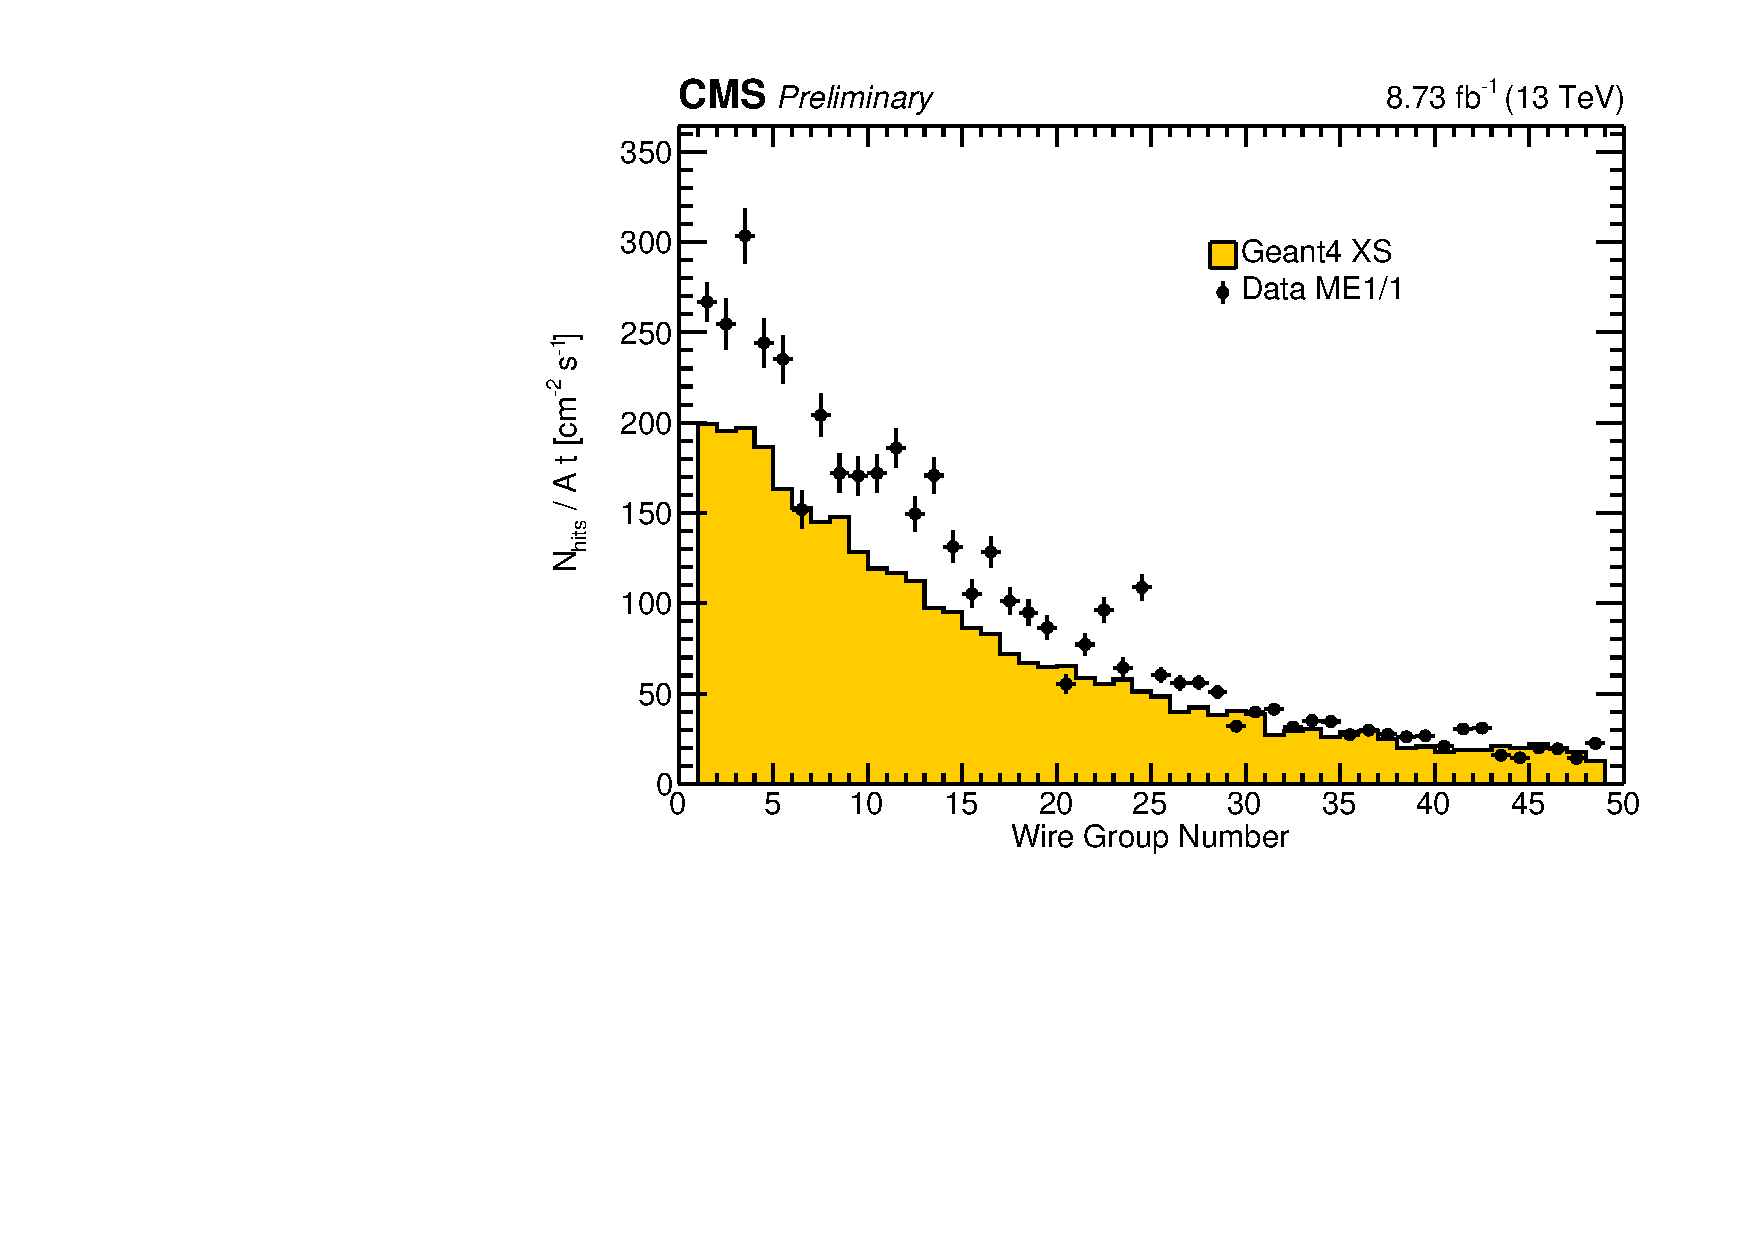
\includegraphics[width=0.85\dummyFigWidth]{figures/neutron/occupancy_11_wire_early_AREA_TIME_20180628_XS_ThermalON.pdf}
	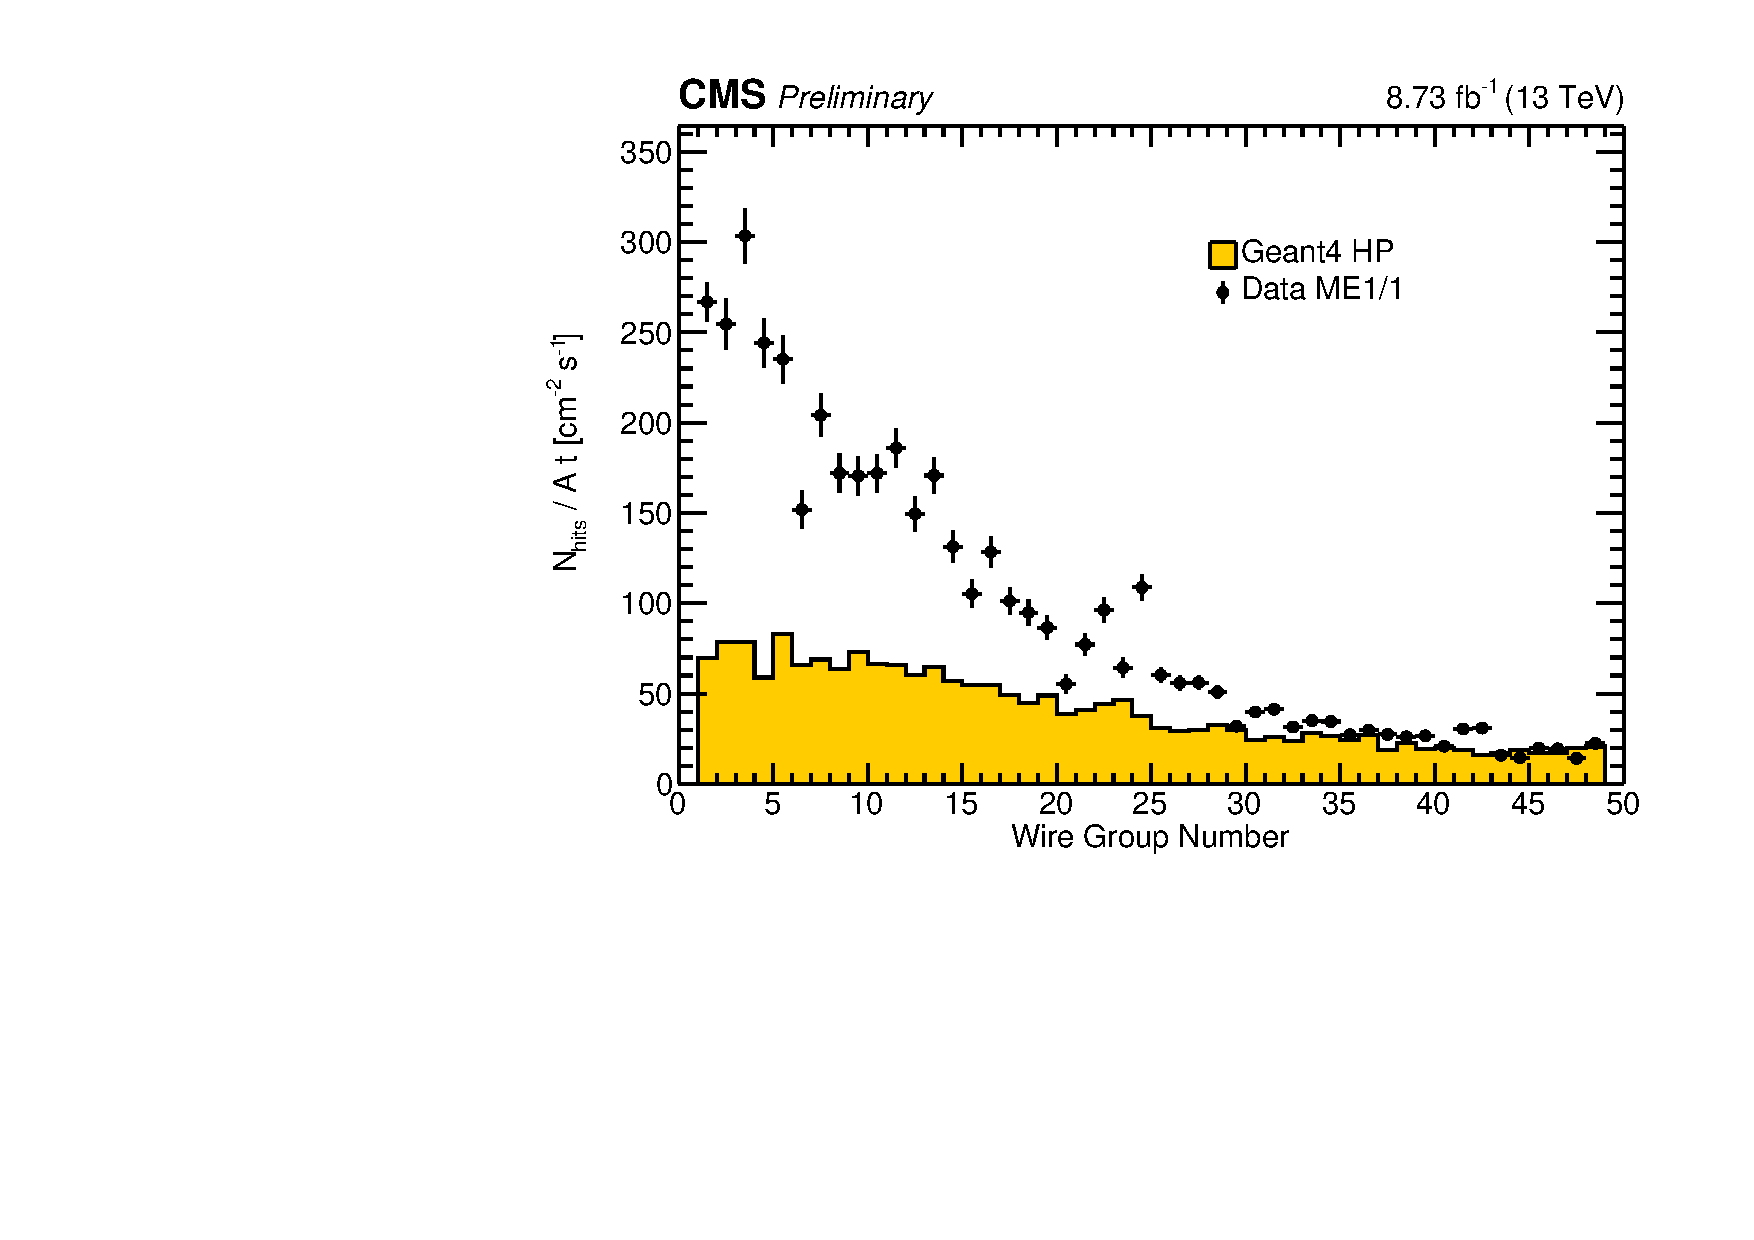
\includegraphics[width=0.85\dummyFigWidth]{figures/neutron/occupancy_11_wire_early_AREA_TIME_20180628_HP_ThermalON.pdf}
  \caption[Histogram of neutron capture induced anode wire hits per time per area for CMS data and for MC simulation for ME1/1 chambers for a reference luminosity of \reflumi.]{Histogram of neutron capture induced anode wire hits per time per area for CMS data (as calculated in \Eq~\ref{eqn:hits_perA_perT_perDigi}) and for MC simulation (as calculated in \Eq~\ref{eqn:MC_hits_perA_perT_perDigi}) for ME1/1 chambers for a reference luminosity of \reflumi. CMS data are compared to results from \GEANTfour (\posstyle{top}) XS and (\posstyle{bottom}) HP neutron interaction cross section libraries in CMS MC simulation of minimum-bias proton-proton collisions at 13 TeV.}
	\label{fig:wg_occupancy_11}
\end{figure}
\begin{figure}[htbp]
	\centering
	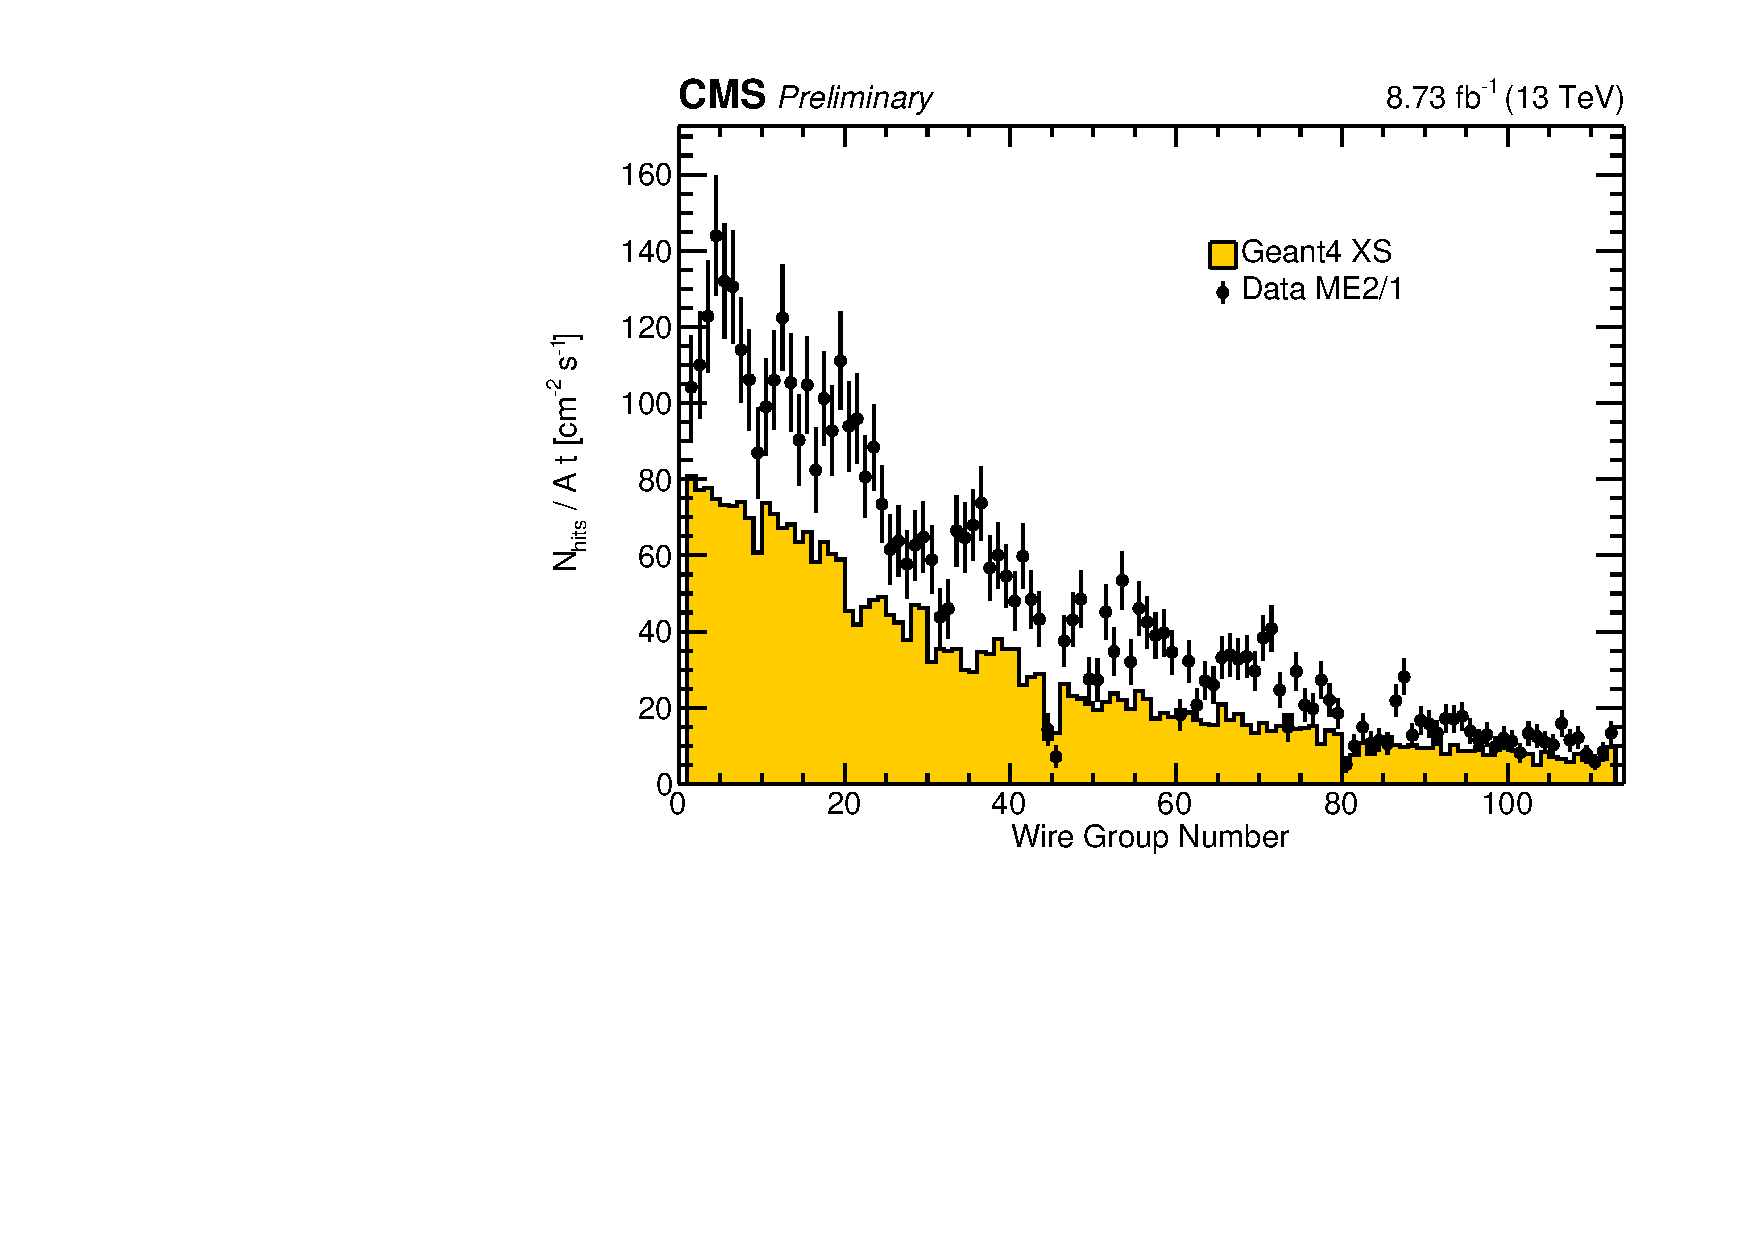
\includegraphics[width=0.85\dummyFigWidth]{figures/neutron/occupancy_21_wire_early_AREA_TIME_20180628_XS_ThermalON.pdf}
	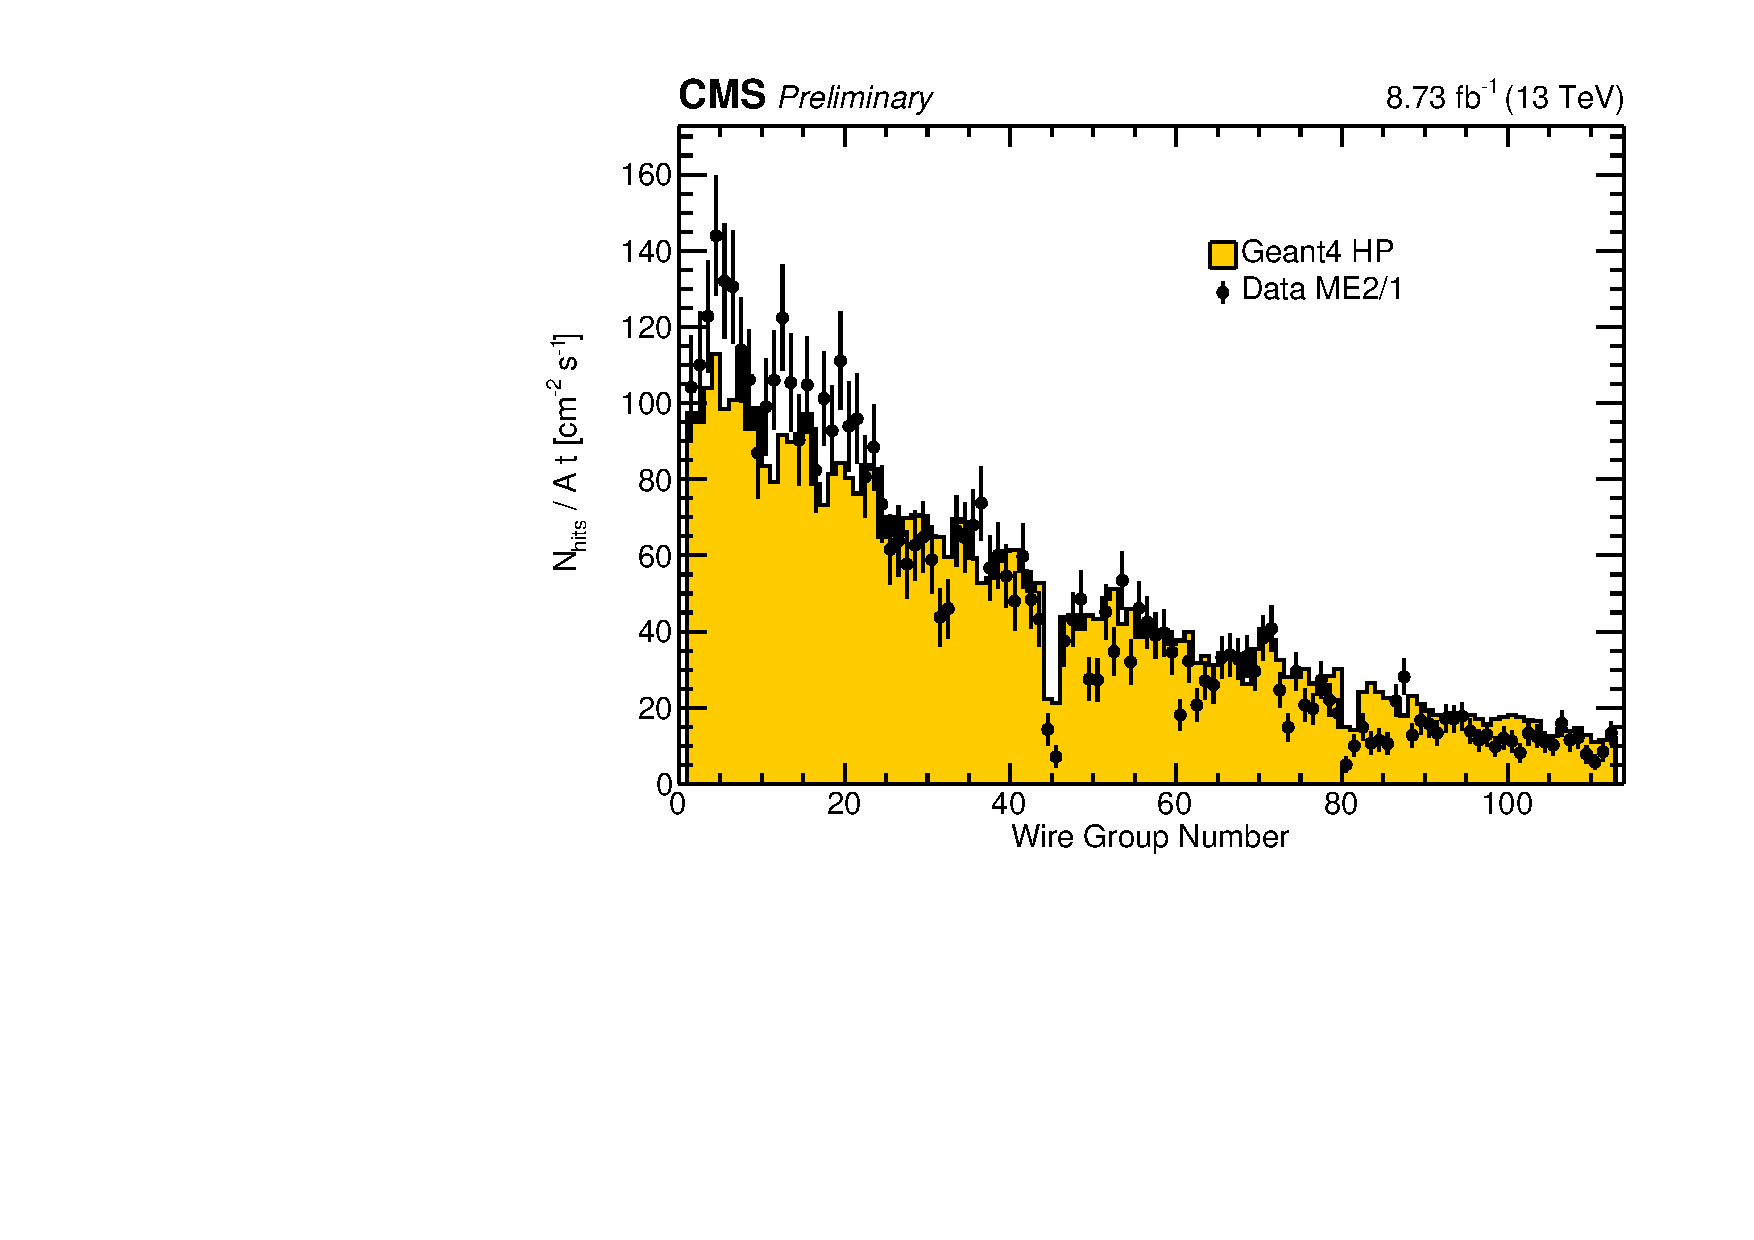
\includegraphics[width=0.85\dummyFigWidth]{figures/neutron/occupancy_21_wire_early_AREA_TIME_20180628_HP_ThermalON.pdf}
  \caption[Histogram of neutron capture induced anode wire hits per time per area for CMS data and for MC simulation for ME2/1 chambers for a reference luminosity of \reflumi.]{Histogram of neutron capture induced anode wire hits per time per area for CMS data (as calculated in \Eq~\ref{eqn:hits_perA_perT_perDigi}) and for MC simulation (as calculated in \Eq~\ref{eqn:MC_hits_perA_perT_perDigi}) for ME2/1 chambers for a reference luminosity of \reflumi. CMS data are compared to results from \GEANTfour (\posstyle{top}) XS and (\posstyle{bottom}) HP neutron interaction cross section libraries in CMS MC simulation of minimum-bias proton-proton collisions at 13 TeV.}
	\label{fig:wg_occupancy_21}
\end{figure}

% Blotting out the appendices for now
%Appendices~\ref{sec:appendix_lumi}, \ref{sec:appendix_occ}, \ref{sec:appendix_phi}, and \ref{sec:appendix_int} contain additional plots of the background hit rates for each of the nine chamber types and for each of the three regions defined by \Tab~\ref{tab:time_windows}. Appendix~\ref{sec:appendix_lumi} contains plots of the hit rate \vs instantaneous luminosity and the hit rate \vs instantaneous luminosity without normalizing to \pp collisions. Appendix~\ref{sec:appendix_occ} contains plots of the local $r$ and $\phi$ distributions. Appendix~\ref{sec:appendix_phi} contains plots of the global $\phi$ distributions. Finally, Appendix~\ref{sec:appendix_int} contains plots of the hit rate \vs CSC chamber type. For candidate neutron capture induced hits in the end-of-gap region, comparisons between CMS data and the HP and XS neutron MC simulations are also shown where appropriate. 

\subsection{Neutron Hit Patterns}
A neutron-induced electron that leaves hits in more than one strip or layer is potentially more disruptive to reconstruction than one that leaves a single isolated hit. It is of interest to see if the MC simulation reproduces digi patterns of single, double, and triple hits found in CMS data. From the selected neutron digis, we consider contiguous clusters of at most 3 half-strips $\times$ 3 layers, \ie $\phi$-$z$ patterns, and study patterns for both CMS data and MC simulation.

\Fig~\ref{fig:pattern} displays histograms of the neutron-induced hit $\phi$-$z$ pattern distribution for CMS data and MC simulation. The $x$~axis bin labels each show a representation of the half-strip \vs layer pattern; the horizontal direction in each is half-strips, and the vertical direction in each is layers. The sections of plots are colored by the number of hits in each pattern; on the far left in green is the only 1-hit pattern, followed by all possible 2-hit patterns in blue, and finally all possible 3-hit patterns in orange. The shaded histogram bins indicate patterns that have comparators on adjacent half-strips on the same layer. Since trigger electronics only report comparator hits on adjacent half-strips if they are in different time bins, the occupancy of these patterns should be suppressed compared to patterns to which they are otherwise geometrically similar. Comparing the shaded histogram bins in \FigDot~\ref{fig:pattern} to the unshaded histogram bins suggests that this is indeed the case.

The distribution of neutron-induced hit patterns is overwhelmingly single, isolated hits. Both the occupancy of each pattern type and the relative ratio between singles, doubles, and triples, as well as to each other, show rough agreement between CMS data and MC simulation.

\begin{figure}[!h]
	\centering
	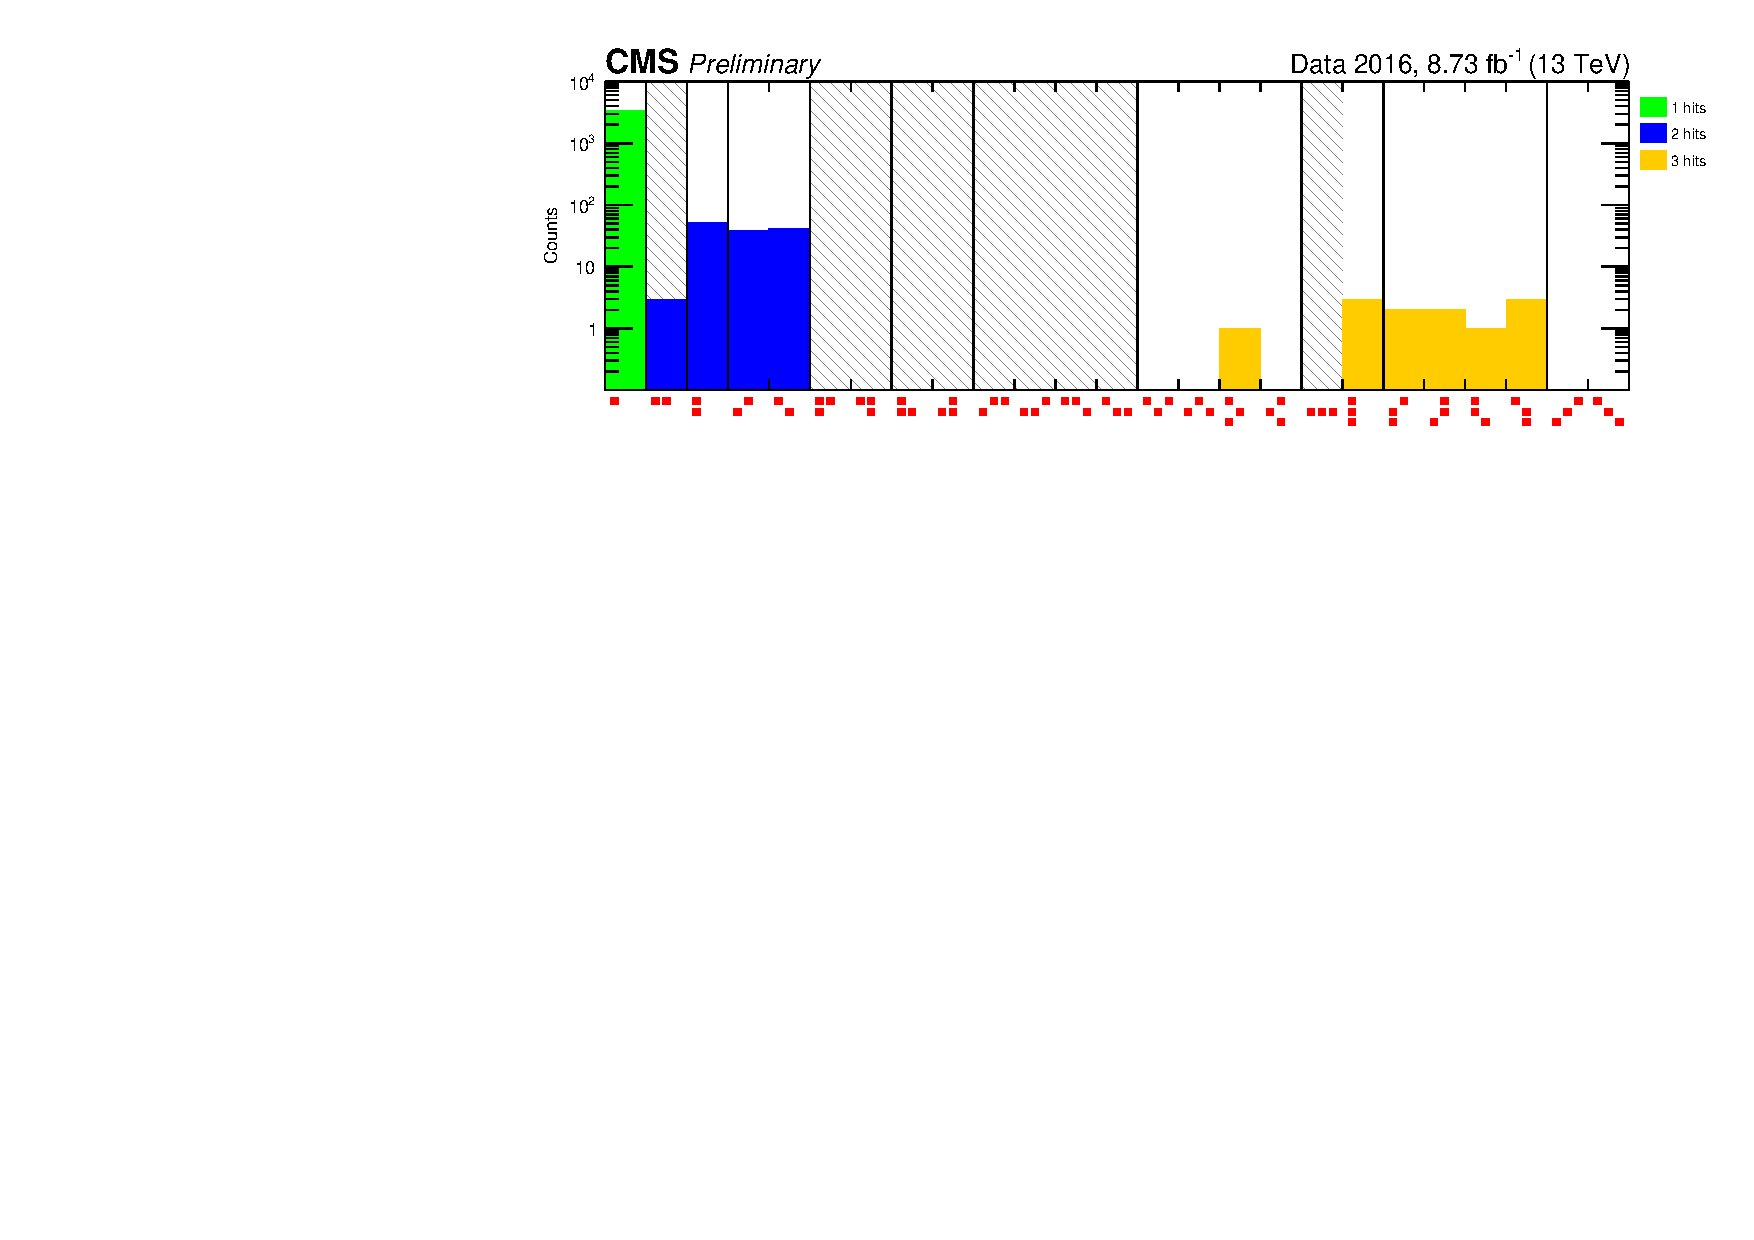
\includegraphics[width=\fullFigWidth]{figures/neutron/BGPatterns_P5.pdf}
	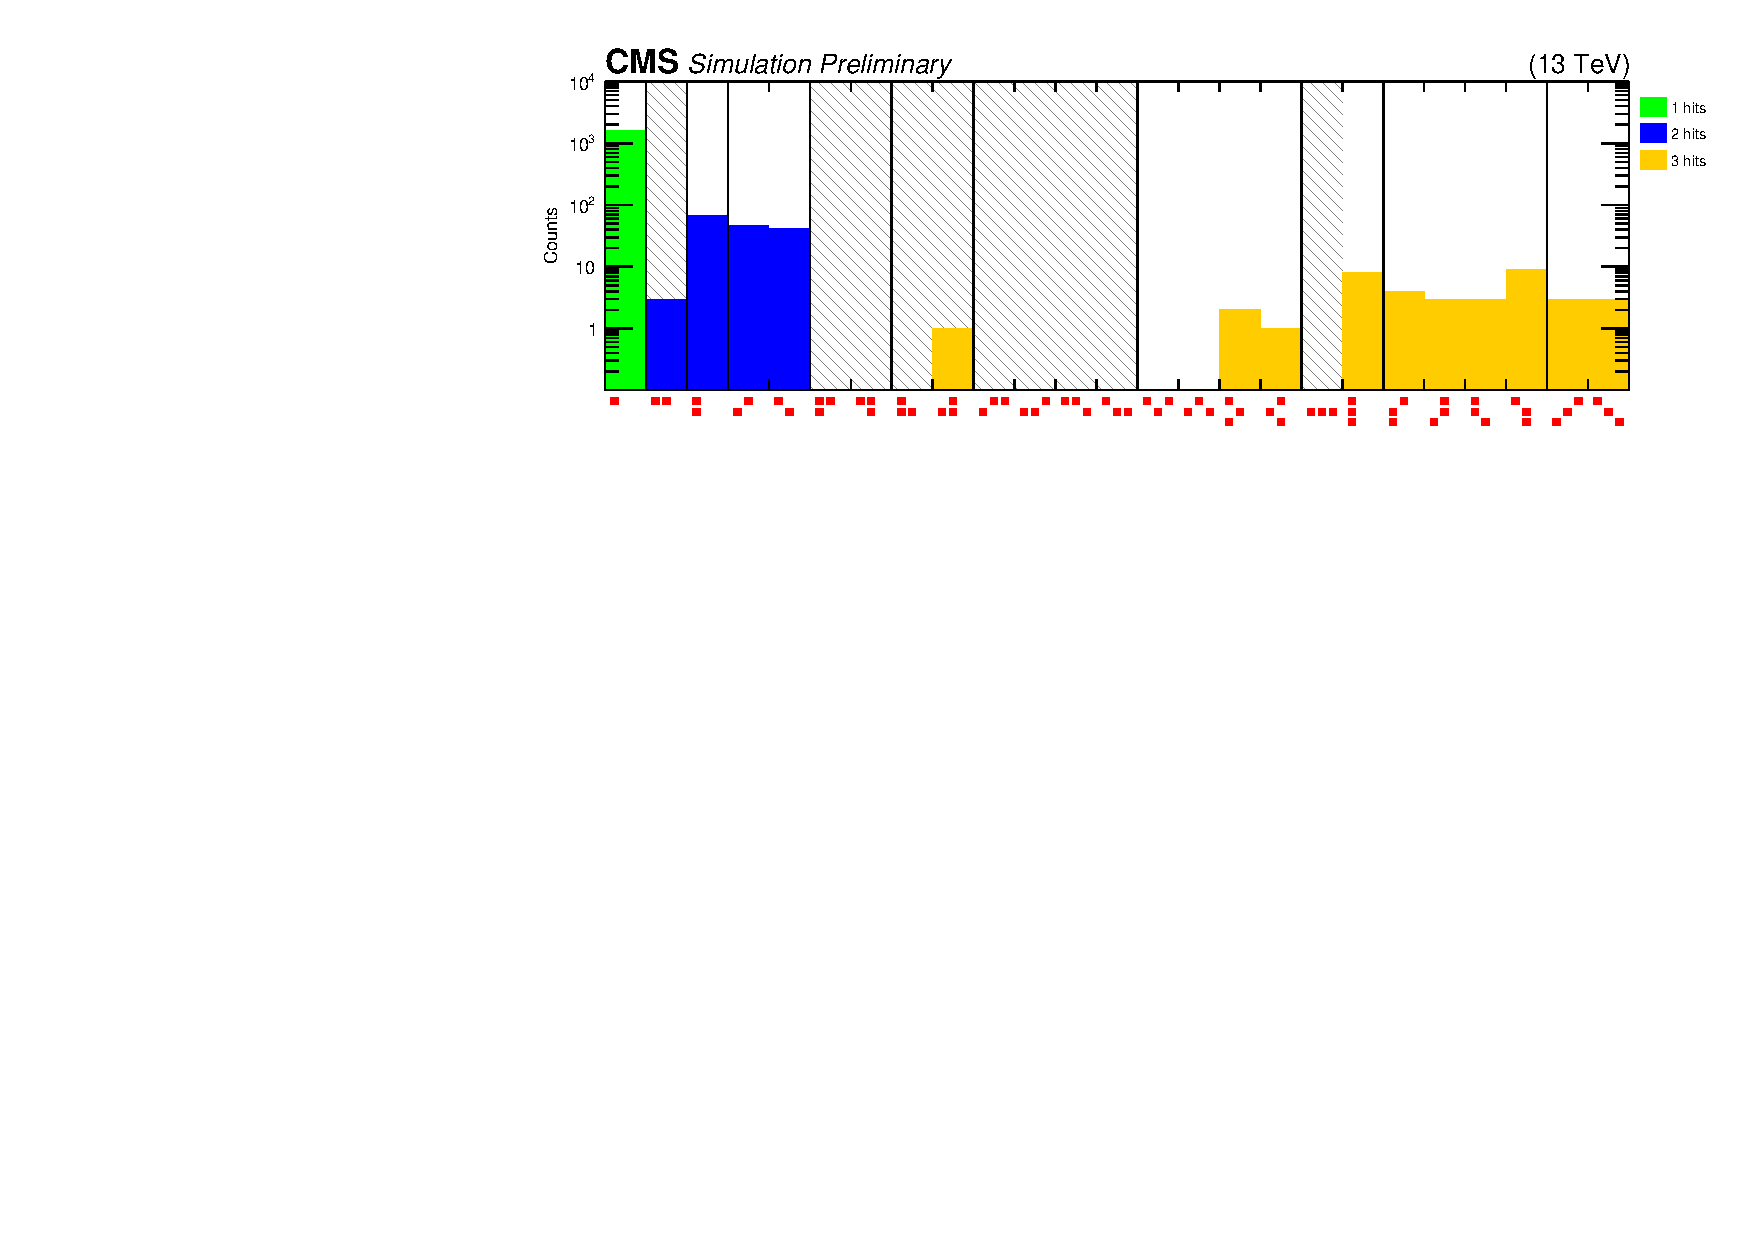
\includegraphics[width=\fullFigWidth]{figures/neutron/BGPatterns_MC.pdf}
  \caption[Distribution of candidate neutron capture induced patterns in 2016 CMS data and CMS simulation.]{Distribution of candidate neutron capture induced patterns in (\posstyle{top}) 2016 CMS data and (\posstyle{bottom}) CMS simulation. The patterns shown here are 1, 2, and 3-hit clusters only. For each red 3$\times$3 pattern, the horizontal direction represents cathode half-strips and the vertical direction represents a layer in the CSC. The red boxes in a pattern indicate the presence of a candidate neutron capture induced hit in a cathode half-strip and layer. The shaded histogram bins correspond to patterns that are suppressed by CSC firmware electronics.}
	\label{fig:pattern}
\end{figure}

\section{Muon Test Beam Studies at GIF++}
\label{sec:GIF}
\subsection{The GIF++ Experimental Setup}
The CERN Gamma Irradiation Facility (GIF++) is located on the CERN Pr\'{e}vessin site in the H4 beam line extracted from the Super Proton Synchrotron (SPS) \cite{Pfeiffer:2016hnl}. The SPS delivers a beam of 400\GeV protons on a fixed target, providing a charged particle beam of hadrons decaying to a beam primarily consisting of muons with a broad momentum spectrum around 100\GeV. The facility includes a 13.9\unit{TBq} \chem{137}{Cs} gamma ray irradiation source emitting primarily 662\keV photons with the means to attenuate the source over a large range. Two CSCs (one ME1/1 and one ME2/1) are placed within the facility. This setup is used for studying aging, gas gain, high-luminosity conditions, \etc, in preparation for the HL-LHC.

\Lone Trigger Accepts (L1As) from muons, triggering chamber readout, can be produced in one of two ways. The first way is by self-trigger, where L1As are produced by chamber electronics forming Local Charged Tracks (LCTs) using coarsely correlated anode wire and cathode strip hits. Variables under control in the experimental setup include the chamber anode high voltage, the gamma ray source intensity (via attenuating filters, allowing a range of intensities from fully open to nearly closed as well as completely off), and the firmware of the controlling electronics, which defines various settings such as hit multiplicity thresholds. The second way to produce L1As is by external trigger, where L1As are produced by the triple coincidence of three scintillators in the beam: one upstream of the source, one downstream of the source, and one that is mounted in the path of the beam just in front of the chambers. The GIF++ data used in this note are externally triggered data taken during a muon test beam over a large range of GIF++ source intensities with CMS-like firmware parameters, and with a set of high voltages intended to equalize gas gain across all layers.

\subsection{LCT Efficiency and RecHit Displacement at GIF++}
\begin{figure}[htbp]
	\centering
	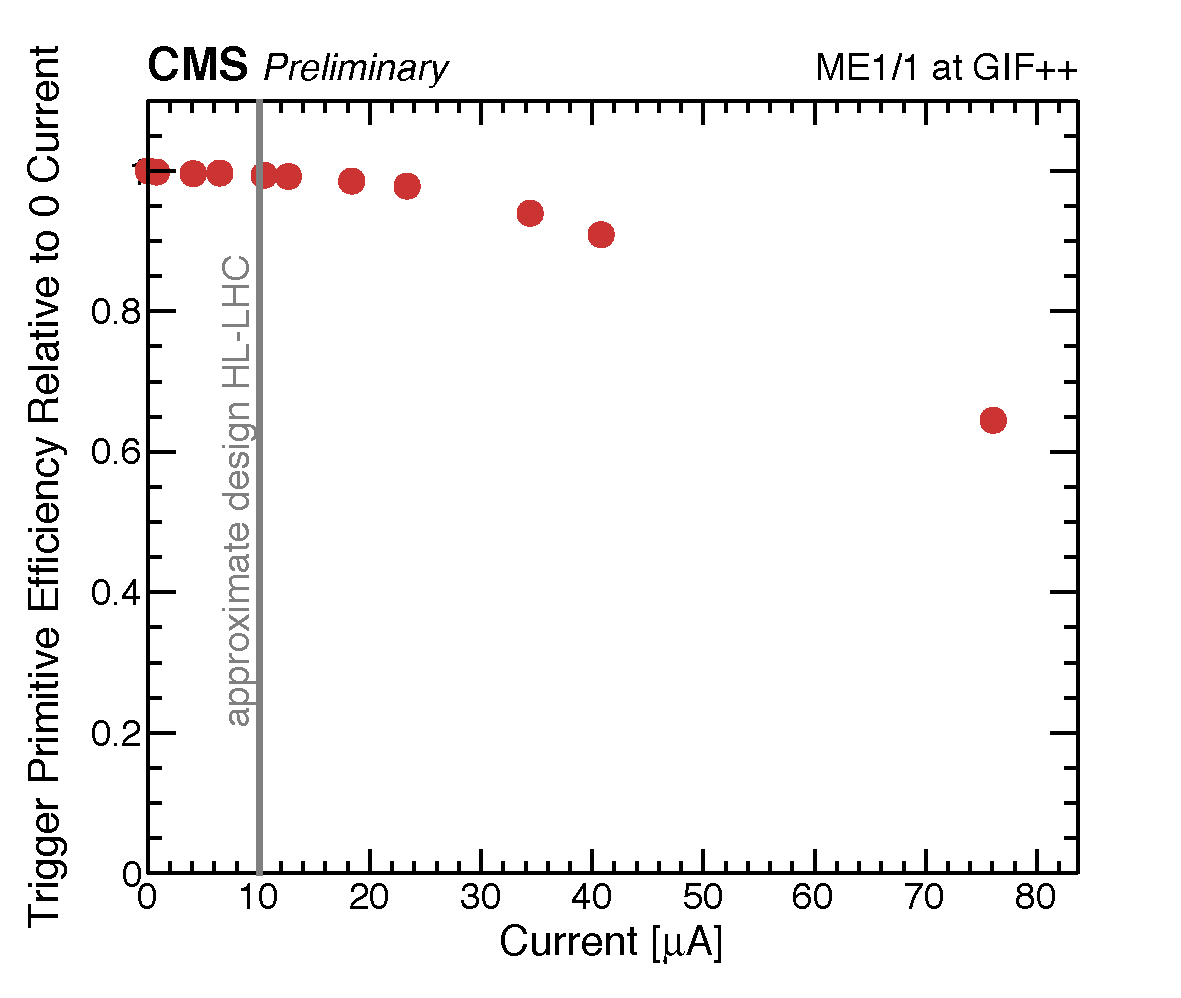
\includegraphics[width=.7\dummyFigWidth]{figures/neutron/Eff_11_LCTScint_L1A.pdf}
	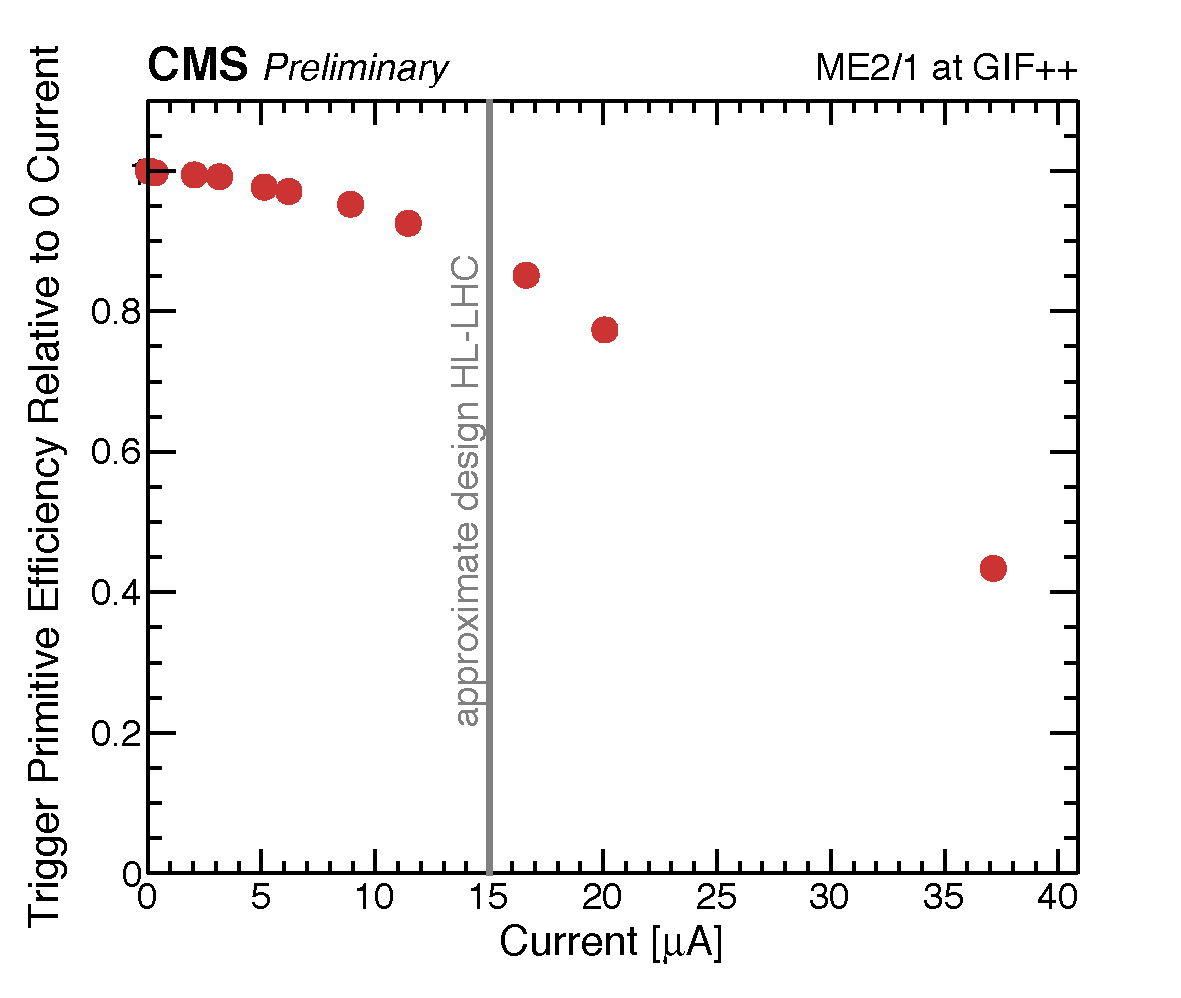
\includegraphics[width=.7\dummyFigWidth]{figures/neutron/Eff_21_LCTScint_L1A.pdf}
  \caption[Plot of LCT efficiency divided by the efficiency at minimum HV current for ME1/1 and ME2/1 chambers at GIF++.]{Plot of LCT efficiency divided by the efficiency at minimum HV current (irradiation source turned off), for the (\posstyle{top}) ME1/1 and (\posstyle{bottom}) ME2/1 chambers at GIF++. LCT efficiency is defined as the number of LCTs created within a scintillator shadow, divided by the number of scintillator triggers received. As the source intensity is increased (chamber anode HV current is increased), the LCT efficiency drops. The gray line indicates an approximate equivalent HV current corresponding to design HL-LHC luminosity.}
	\label{fig:lct_eff}
\end{figure}

To measure the LCT efficiency, we begin by counting the fraction $f$ of L1As that have at least one LCT within the area shadowed by the middle scintillator mounted in front of the chambers. Due to issues of precisely defining the shadow and dealing with events with more than one muon, we do not attempt to define an absolute efficiency. Instead, we define a relative efficiency dividing the value of $f$ taken at higher source intensities by the value of $f$ with the GIF++ source off, denoted $f_\text{off}$. We estimate the scintillator area boundary empirically using a position scatter plot of LCTs, and count those LCTs whose layer 3 half-strip and wire group number fall within this boundary. \Fig~\ref{fig:lct_eff} displays plots of the LCT relative efficiency, $f/f_\text{off}$, as a function of chamber anode HV current induced by increasing the GIF++ source intensity for the ME1/1 and ME2/1 chambers at GIF++. As the gamma source intensity is increased, the number of photon-induced noise hits increases, and the number of LCTs constructed decreases.

%We identify two possible causes for the decrease in the number of LCTs created. The first possibility is that signal muon LCTs are lost due to the chamber electronics spending too much time processing a large number of low quality LCTs, causing signal LCTs to be missed. This phenomenon is referred to as dead time. The second possibility is that signal muon LCTs are lost due to corrupted hits induced by background. To study the first possibility, we tightened the threshold for the number of hits required to create a pre-trigger. \fixmeCOMMENTED{explain pre-trigger better} Muon LCTs are typically of high quality, consisting of five or six hits, so if the loss were indeed due to dead time, tightening the pre-trigger threshold would result in the electronics processing fewer low quality background LCTs, decreasing dead time, which in turn would decrease the chance of missing a high quality signal muon LCT. If on the other hand the electronics are not being saturated with high background rates, tightening the pre-trigger threshold would simply further decrease the number of LCTs constructed.

%\begin{figure}[htbp]
%	\centering
%	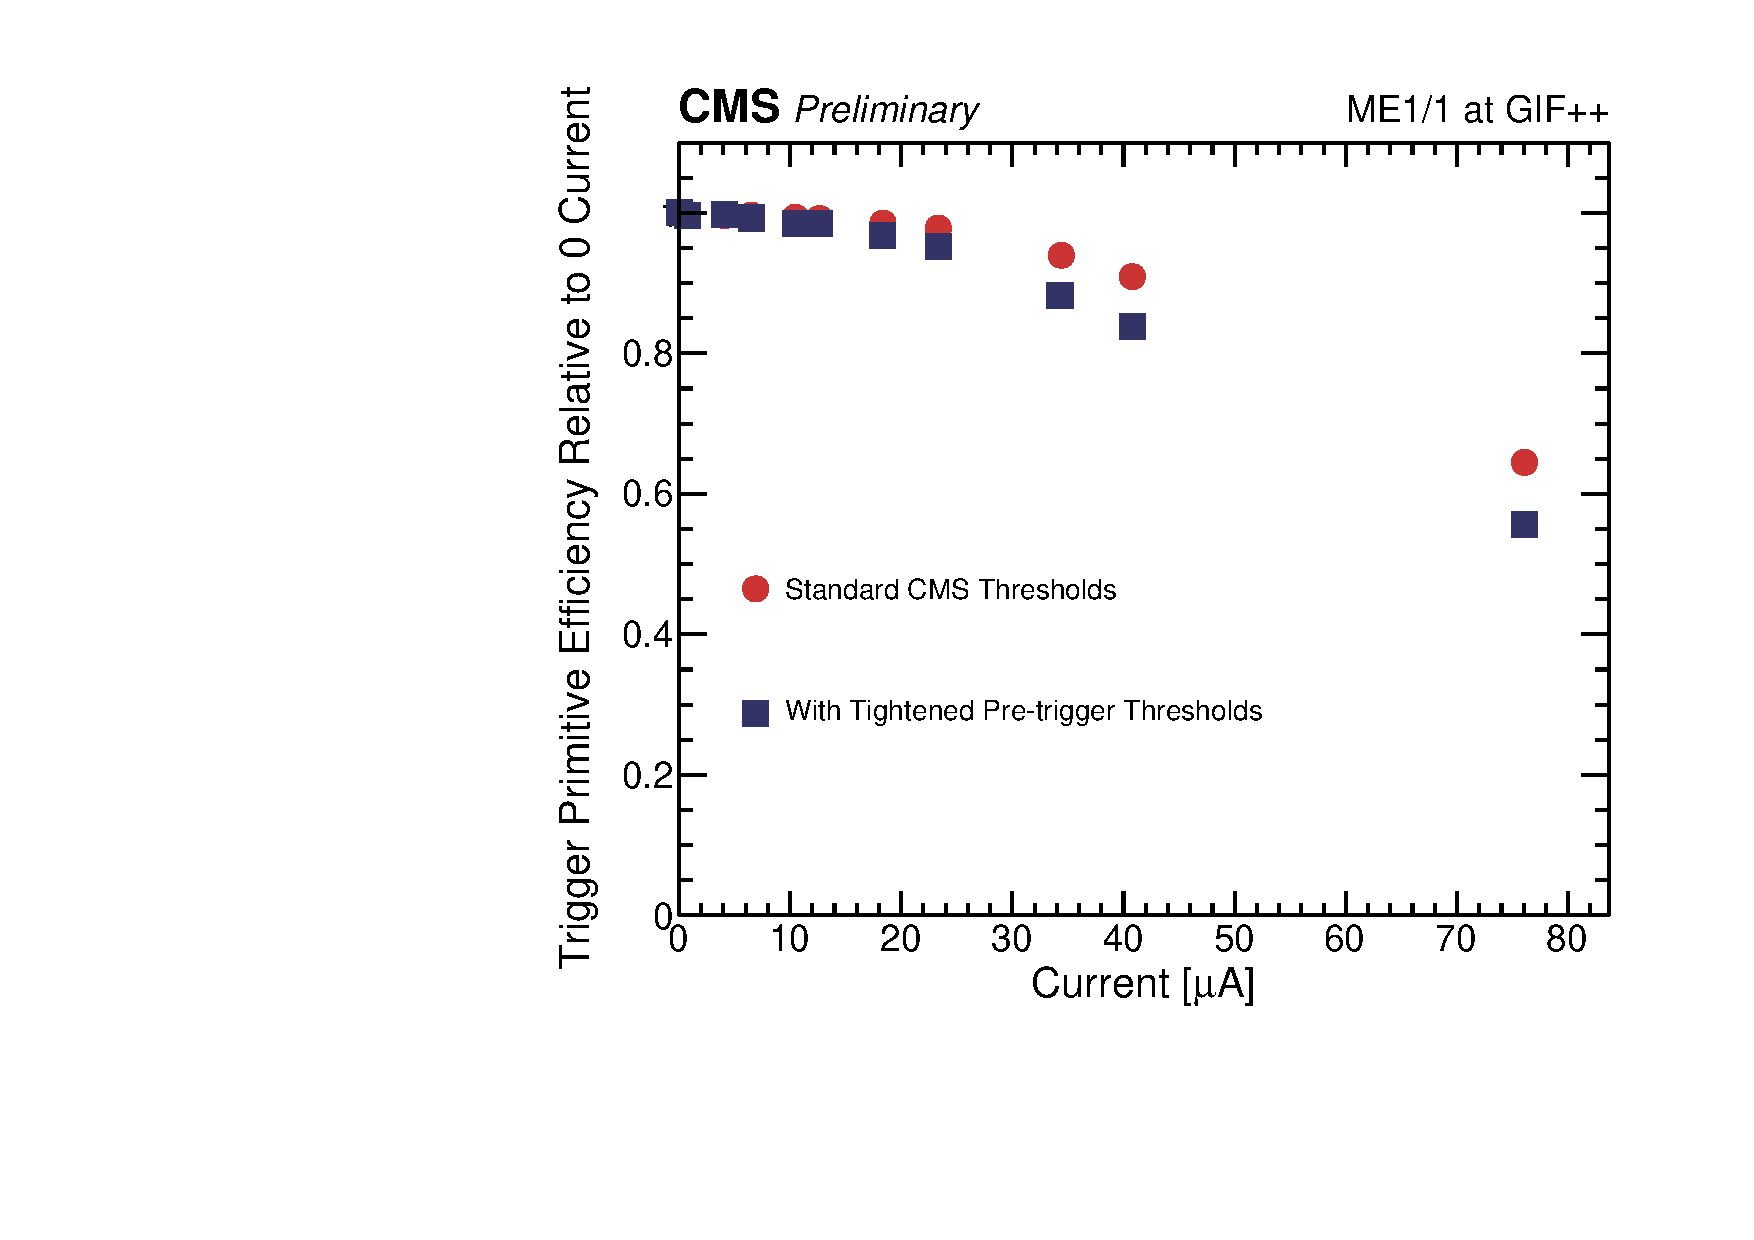
\includegraphics[width=\dummyFigWidth]{figures/neutron/Eff_11_withTight.pdf}
%	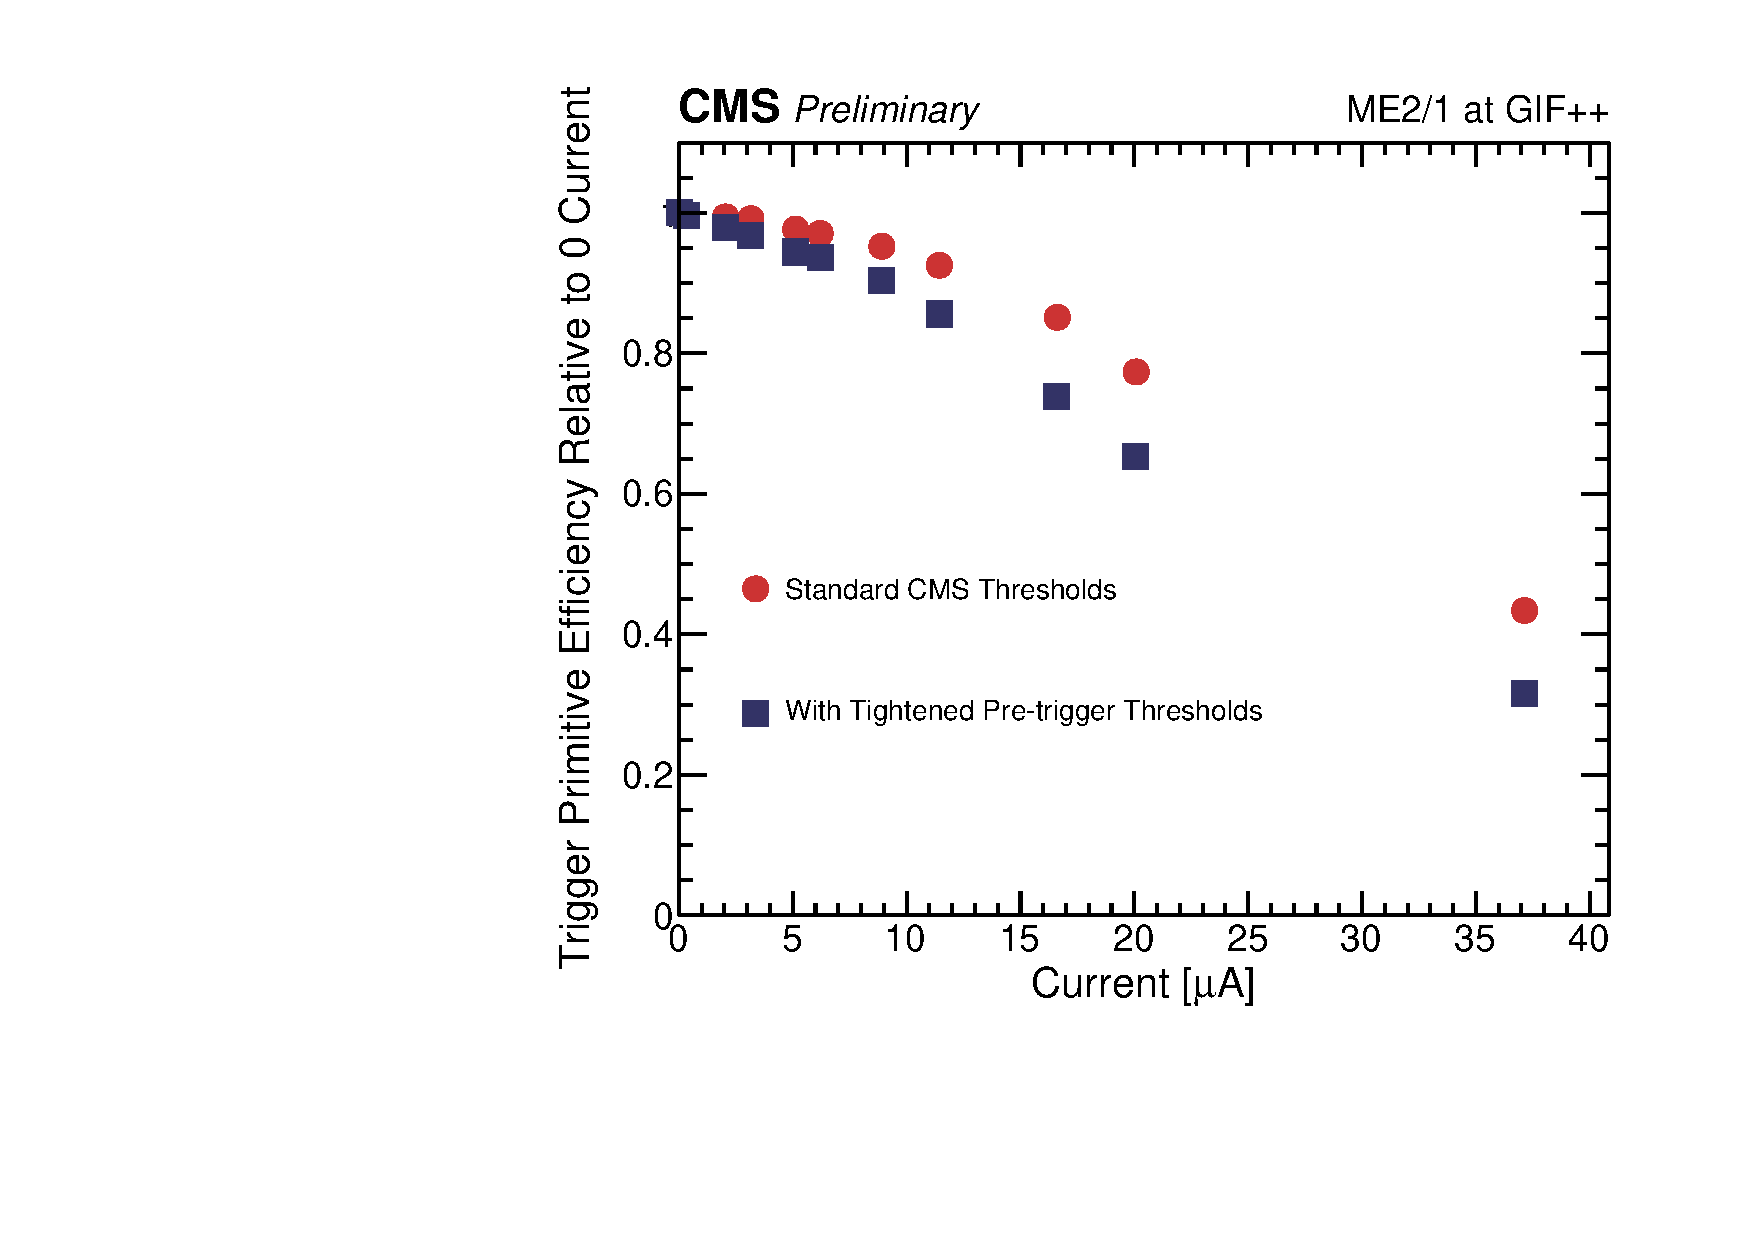
\includegraphics[width=\dummyFigWidth]{figures/neutron/Eff_21_withTight.pdf}
%	\caption{LCT efficiency divided by the efficiency at minimum chamber current, with and without tightened pre-CLCT hit multiplicity threshold for (\posstyle{top}) ME1/1 and (\posstyle{bottom}) ME2/1}
%	\label{fig:lct_eff_withTight}
%\end{figure}

%Figure~\ref{fig:lct_eff_withTight} displays two plots of LCT efficiency divided by the efficiency at minimum chamber current (GIF++ source off), as a function of chamber anode current for the ME1/1 and ME2/1 chambers at GIF++. The red circles are data taken with the same hit thresholds as CMS, and the blue squares are data taken with the CLCT pre-trigger threshold tightened by one hit, \ie the requirement was tightened from 3 hits to 4 hits. \fixmeCOMMENTED{not convincing} The LCT efficiency at a given current is strictly lower in data taken with the tightened pre-trigger threshold, compared to the CMS threshold. We therefore infer that dead time is not a significant source of LCT efficiency loss, and turn to the second possibility: that the LCT efficiency loss is due to corrupted hits.

\begin{figure}[htbp]
	\centering
	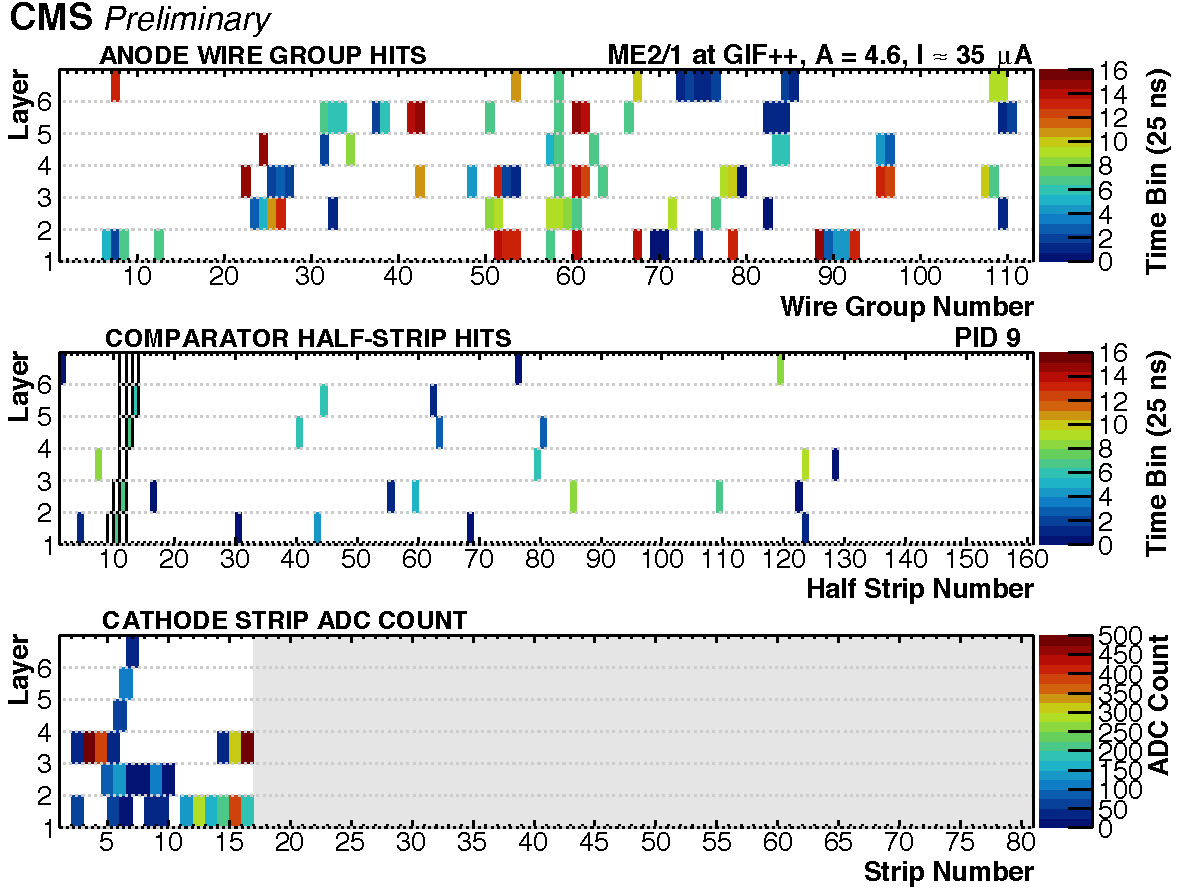
\includegraphics[width=\dummyFigWidth]{figures/neutron/ED_GIF_3384_ME21_9.pdf}
  \caption[Display of an event collected during a muon test beam at the CERN Gamma Irradiation Facility (GIF++) with a CSC from ME2/1.]{Display of an event collected during a muon test beam at the CERN Gamma Irradiation Facility (GIF++) with a CSC from ME2/1, showing digitized detector responses: anode wire ($r$ coordinate) responses (wire group hits), cathode half-strip ($\phi$ coordinate) responses (comparator half-strip hits), and cathode strip analog-to-digital-converter (ADC) counts proportional to deposited charge. Each display is organized by the gas gap layer and the strip or wire number in which the response occurred. The quantity A represents the attenuating factor applied to the 13.9\unit{TBq} \chem{137}{Cs} gamma irradiation source and I is the chamber anode wire HV current. This display illustrates a mechanism by which a photon hit can displace a muon hit; the large amount of deposited charge seen at the left edge of the ADC counts resulted in a corresponding shifted comparator hit.}
	\label{fig:ed}
\end{figure}

\begin{figure}
	\centering
	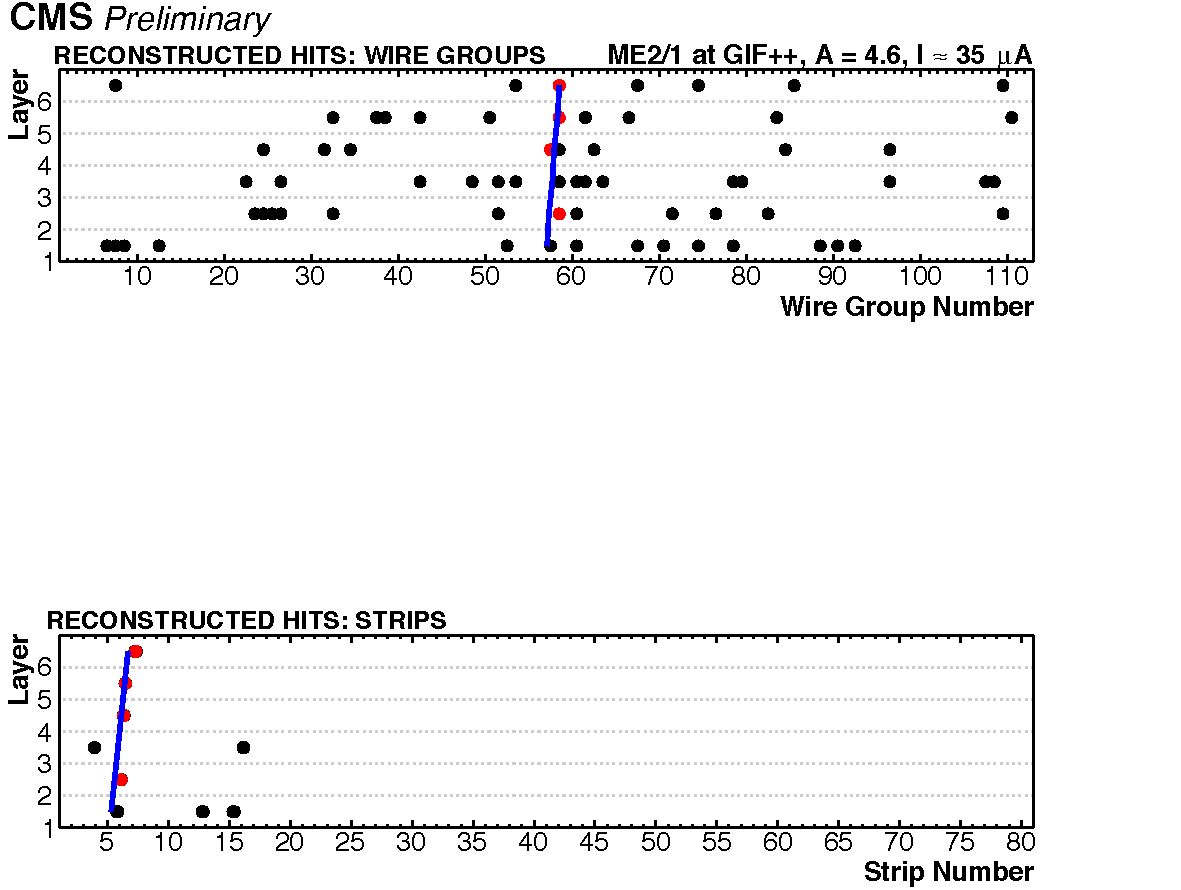
\includegraphics[width=\dummyFigWidth]{figures/neutron/RH_GIF_3384_ME21_9.pdf}
  \caption[Display of the same event, showing offline reconstructed detector responses (RecHits).]{Display of the same event as \FigDot~\ref{fig:ed}, showing offline reconstructed detector responses (RecHits), projected along the anode wire axis and the cathode strip axis (black dots). Blue lines indicate the offline reconstructed muon segment created by a straight-line fit to the red highlighted RecHits. This display illustrates a mechanism by which a photon hit can displace a muon hit; the reconstructed hit in layer 3 was displaced and subsequently excluded from the segment fit.}
	\label{fig:rh}
\end{figure}

One possible cause for the loss of signal muon LCTs is the corruption of muon hits induced by background. To understand the characteristics of hit corruption, we examine CSC event displays such as in \FigDot~\ref{fig:ed}. These event displays show wire group hits, comparator half-strip hits, and strip ADC counts with the layer on the vertical axis and the digi number on the horizontal axis. The color for the wire groups and comparators indicates the digi time bin, while the color for the strip ADC counts indicates the ADC counts. The comparator hit plot has an overlay in black rectangular outline of the LCT pattern that was used to identify the LCT.

This particular event display illustrates a way that a photon-induced hit may cause loss of LCTs, and consequently, loss of offline reconstructed segments. The display shows a muon triggering readout and forming a 4-hit LCT, whose comparator pattern can be seen in half-strips 9--13. The strip ADC counts show a large energy deposit that we attribute to a photon-induced hit in strips 3--4 in layer 3. The corresponding comparator hit in half-strip 7 is shifted away from what would have been its correct position in approximately half-strip 11. This results in what would have been a 5-hit LCT deteriorating to a 4-hit LCT. This ability of photon hits to displace hits can in this way cause loss of LCTs as well as deterioration of their quality.

\Fig~\ref{fig:rh} is a display of the corresponding offline reconstructed hits (RecHits) \cite{Barashko:2007zz}, along with an overlay of the muon segment constructed from them. The RecHits that contributed to the segment are shown in red. The shifted comparator hit and the photon energy deposit resulted in a RecHit that was displaced to the left, resulting in its exclusion from the segment. This directly results in a deterioration of segment reconstruction resolution.

\begin{figure}[htbp]
	\centering
	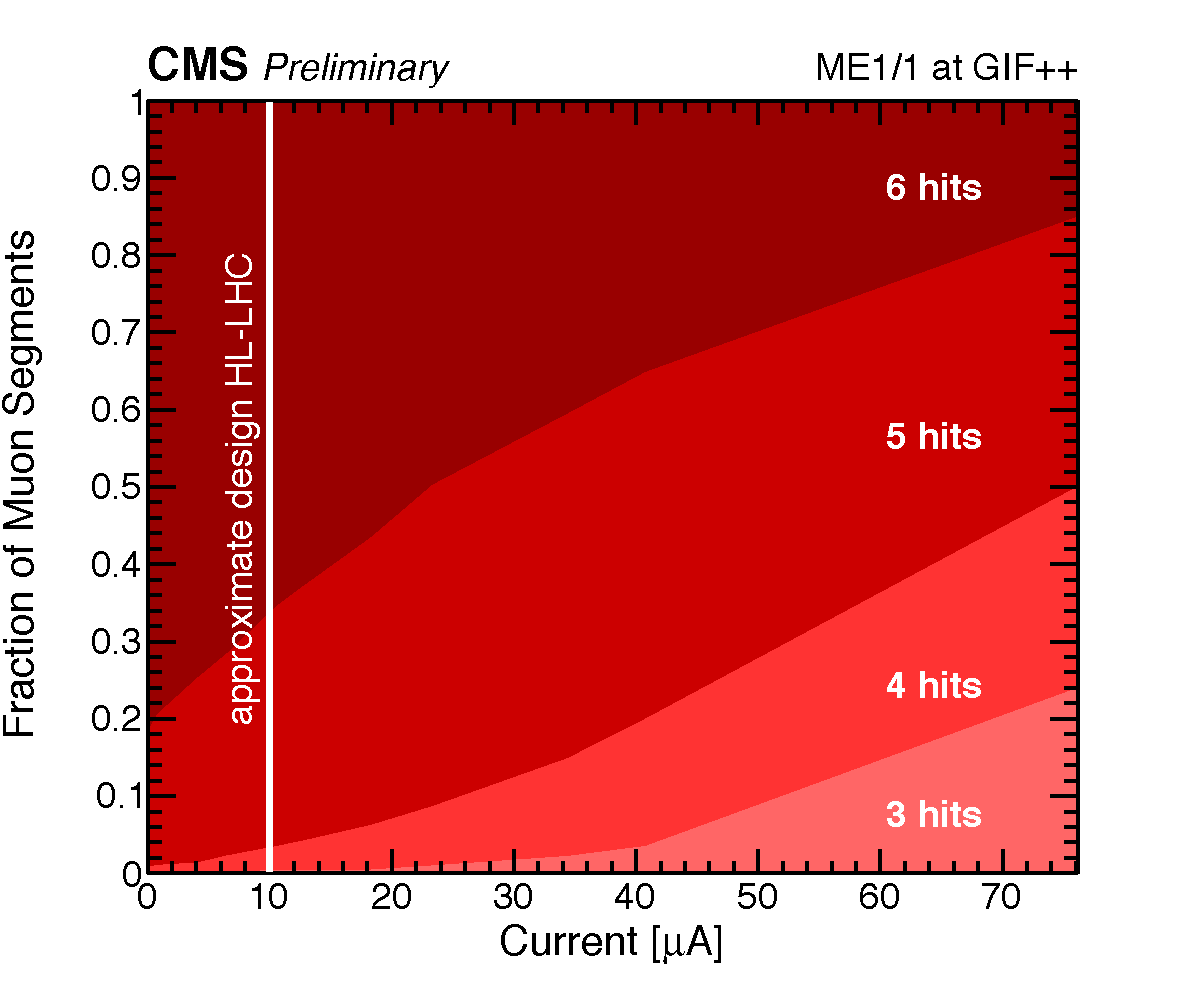
\includegraphics[width=.7\dummyFigWidth]{figures/neutron/SegNHitsFrac_ME11_all.pdf}
	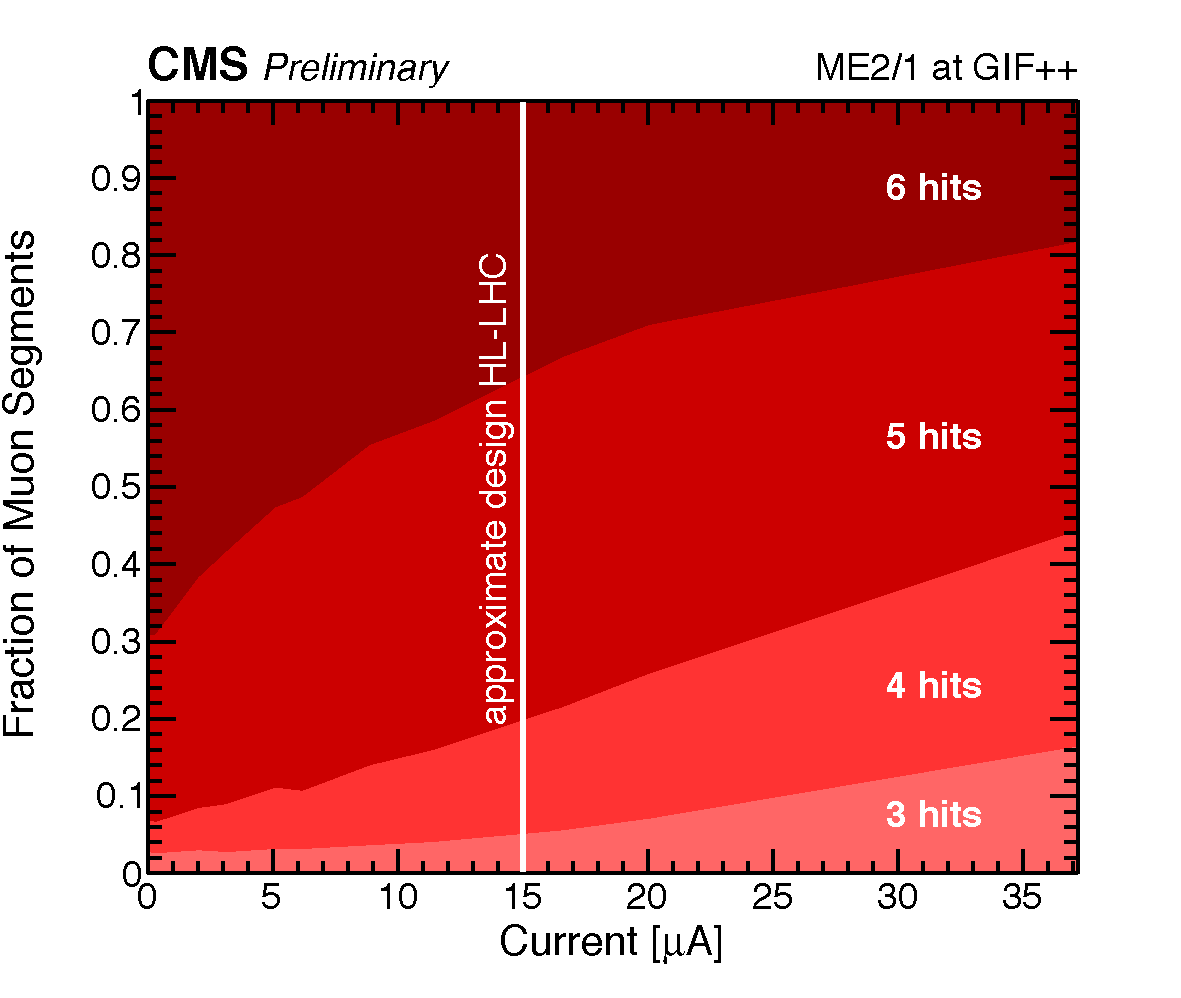
\includegraphics[width=.7\dummyFigWidth]{figures/neutron/SegNHitsFrac_ME21_all.pdf}
  \caption[Stacked plot of fraction of offline reconstructed muon segments, categorized by the number of reconstructed hits used to form them, for the ME1/1 and ME2/1 at GIF++.]{Stacked plot of fraction of offline reconstructed muon segments, categorized by the number of reconstructed hits used to form them, \vs chamber anode HV current, for the (\posstyle{top}) ME1/1 and (\posstyle{bottom}) ME2/1 at GIF++. As the source intensity is increased (chamber anode HV current is increased), the fraction of good quality 6 hit segments decreases, while the fraction of lower quality 3 hit segments increases. The white line indicates an approximate equivalent HV current corresponding to design HL-LHC luminosity.}
	\label{fig:seg_frac}
\end{figure}

\Fig~\ref{fig:seg_frac} displays stacked plots of the fraction of reconstructed muon segments spatially closest to muon LCTs within the scintillator acceptance area, categorized by the number of hits used to form that segment, as a function of chamber anode HV current for the ME1/1 and ME2/1 chambers at GIF++. The plot shows that the fraction of high quality segments formed with 6 hits decreases as the source intensity is increased, while the fraction of lower quality segments formed by 3 hits increases. This confirms that LCT loss can be caused by a loss of hits, and demonstrates the mechanism by which neutron-induced hits can potentially disrupt CSC detector performance.

\section{Charge per Hit Studies at GIF++ and in CMS Data and Simulation}
\label{sec:chargeperhit}

As discussed in \Sec~\ref{sec:GIF}, the GIF++ facility allows us to study the performance of CSC online and offline reconstruction under conditions that potentially correspond to the radiation environment expected at the HL-LHC. To investigate the correspondence between GIF++ source intensity and LHC instantaneous luminosity, we examine the CSC anode HV current as measured by an ammeter in the CSC HV power supply (HVPS) of both CSCs at GIF++ and for similar chamber types at CMS.

eifferences in radiation environments produced from the GIF++ source and from LHC \pp collisions necessitate understanding the validity of using anode HV current for the correspondence between GIF++ and CMS. As noted in \Sec~\ref{sec:GIF} above, GIF++ photons are emitted with a maximum energy of 662\keV by the \chem{137}{Cs} source, and the resulting ionizing electrons are primarily from Compton scattering and the photoelectric effect. In contrast, photons originating from the neutron background in CMS can carry up to several \MeVns in energy and thus, in addition to more energetic electrons from Compton scattering and the photoelectric effect, ionizing electrons and positrons can arise from pair production. Because of these differences and to explore any others, we measure the\unit{charge/hit} of background hits that are expected to be the dominant source of charge in the anode HV current by measuring the ratio of the anode HV current to the anode wire group\unit{hits/s} in both CMS data and GIF++ data. 

\subsection{Computation of charge/hit from CMS data}

\subsubsection{ME1/1}
To calculate\unit{charge/hit} in ME1/1 chambers using CMS data, we take the ratio of the measured HV current (\unit{charge/s}) and the anode wire group\unit{hits/s}. Each of the measured HV current and anode wire group\unit{hits/s} are calculated at a fixed reference luminosity intended to be representative of a typical measured values of the HV current and\unit{hits/s}. We choose \reflumi as the reference luminosity.

We use anode HV current data collected by the HVPS and stored in an external database during LHC fills to calculate the HV current at the reference luminosity, which we refer to as the reference HV current. We read the HV current data offline from the database and correlate each HV current measurement by time to the corresponding measured LHC luminosity. In ME1/1 chambers, each layer constitutes an HV channel. We retrieve the HV current measurements for all ME1/1 HV channels, for all LHC fills during data taking period Run 2016H. We then study plots of anode HV current \vs luminosity and attempt to calculate the reference HV current by performing a two-parameter linear fit to the data and reading off the value of the fit at \reflumi. 

\begin{figure}
	\centering
	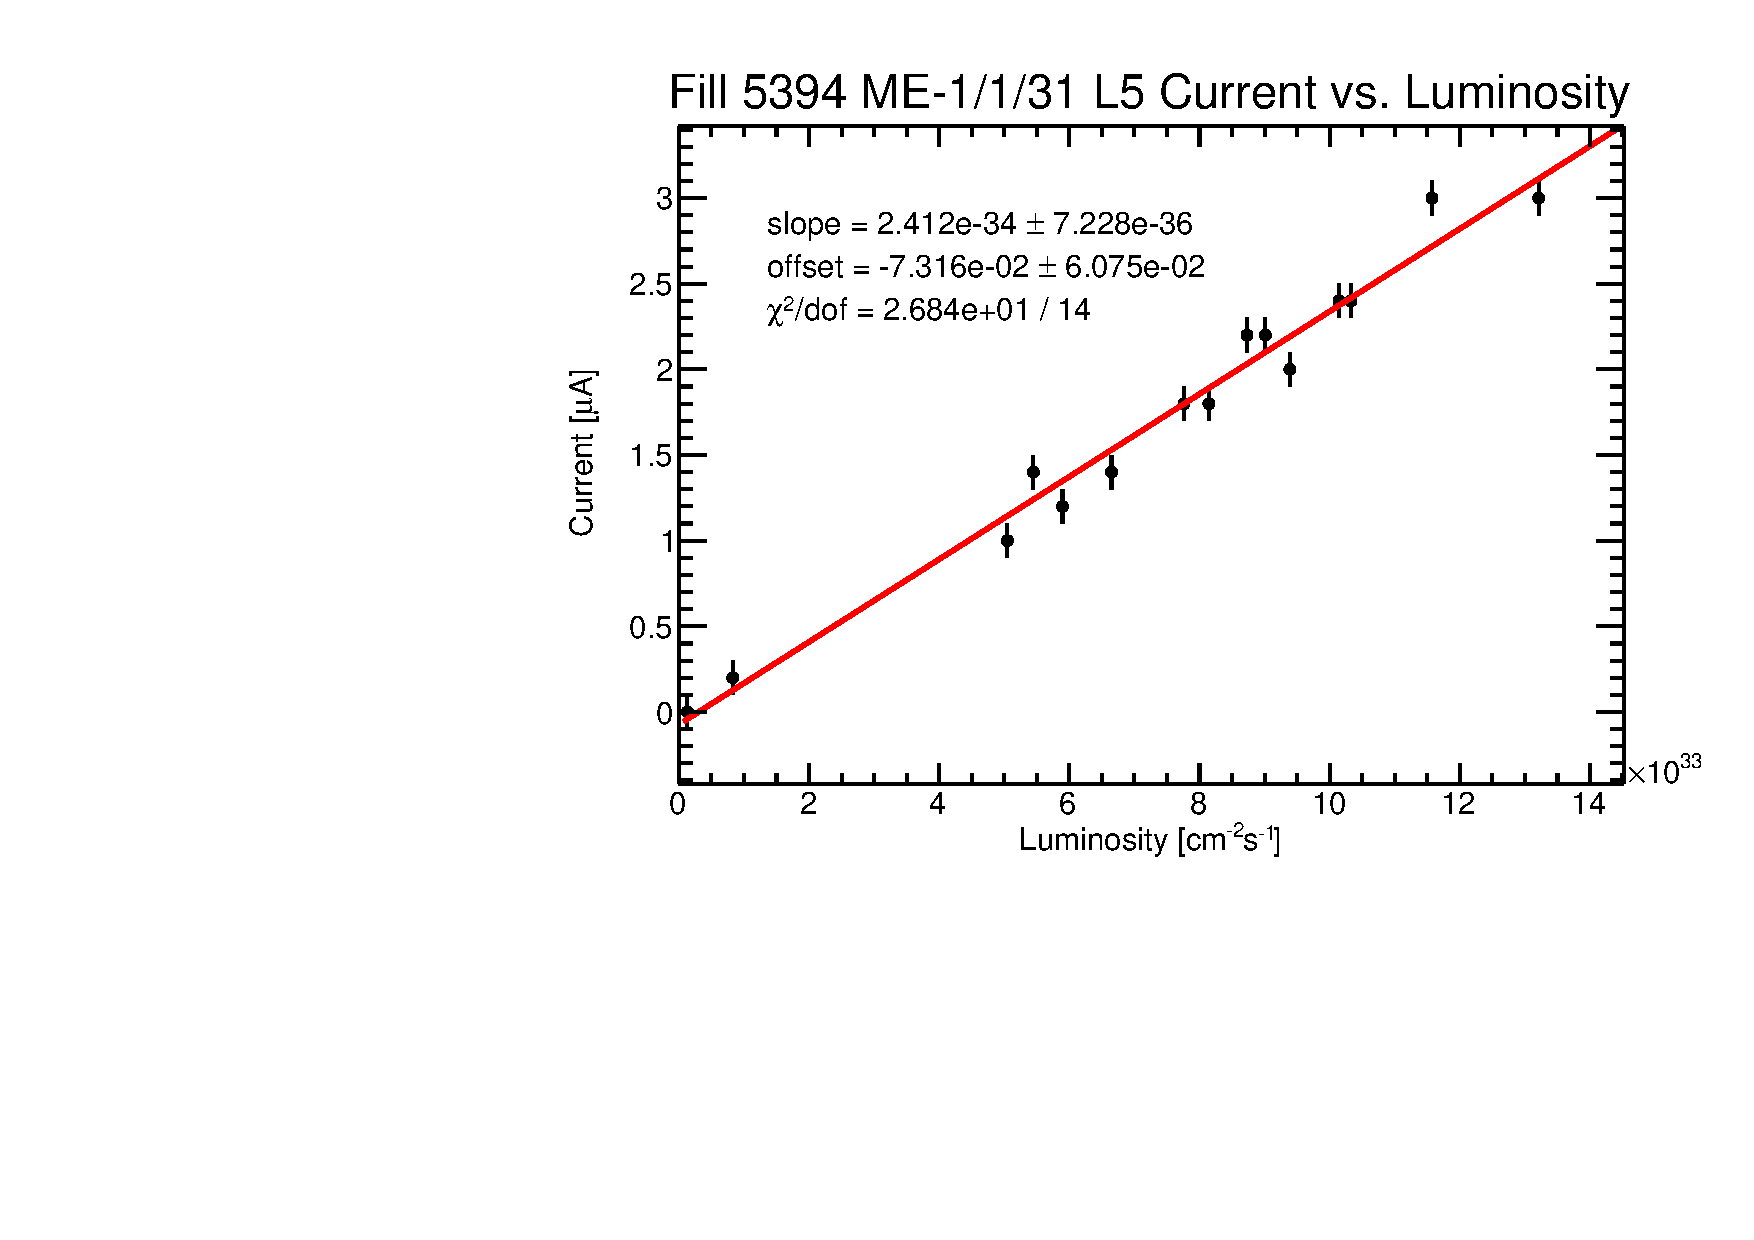
\includegraphics[width=0.7\twoThirdsFigWidth]{figures/neutron/ME11_N_31_5_f5394_curr_lumi.pdf}
	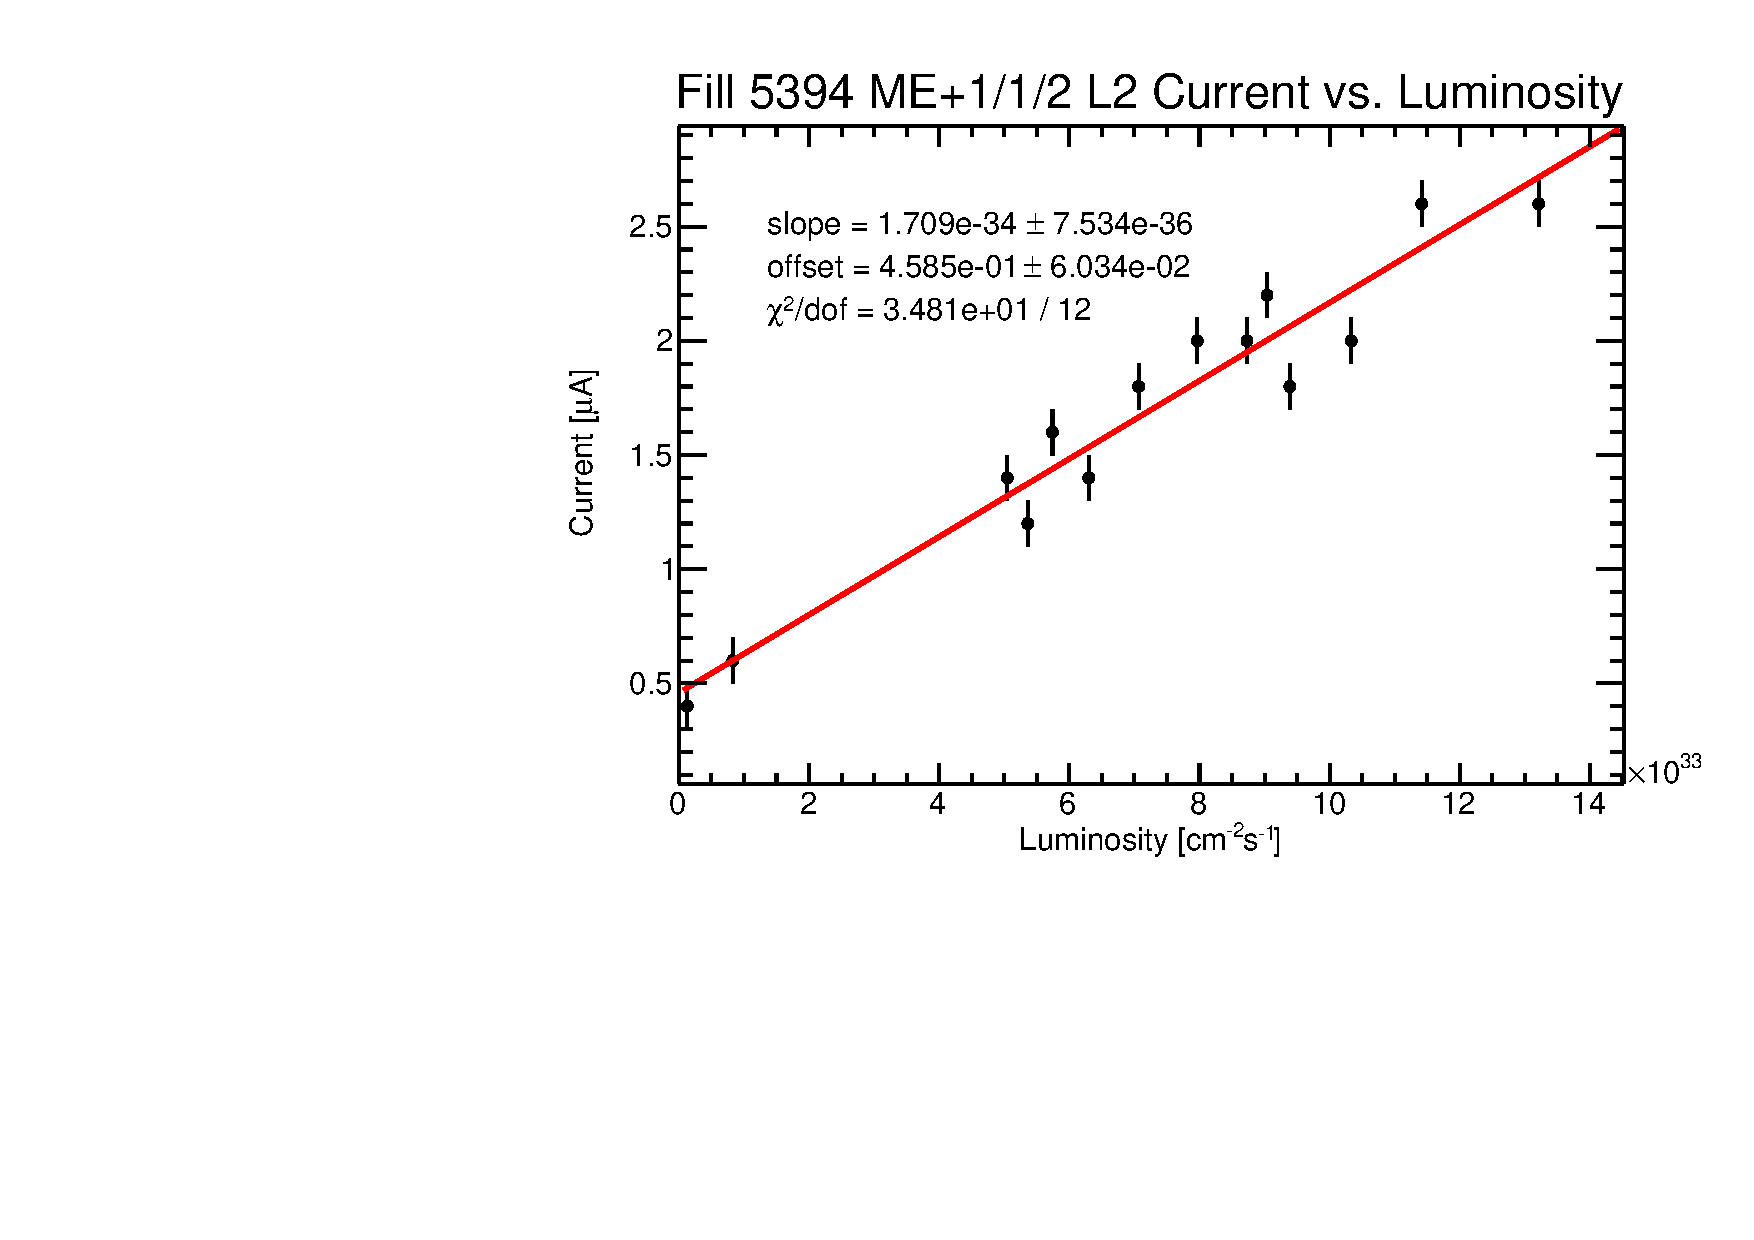
\includegraphics[width=0.7\twoThirdsFigWidth]{figures/neutron/ME11_P_02_2_f5394_curr_lumi.pdf}
	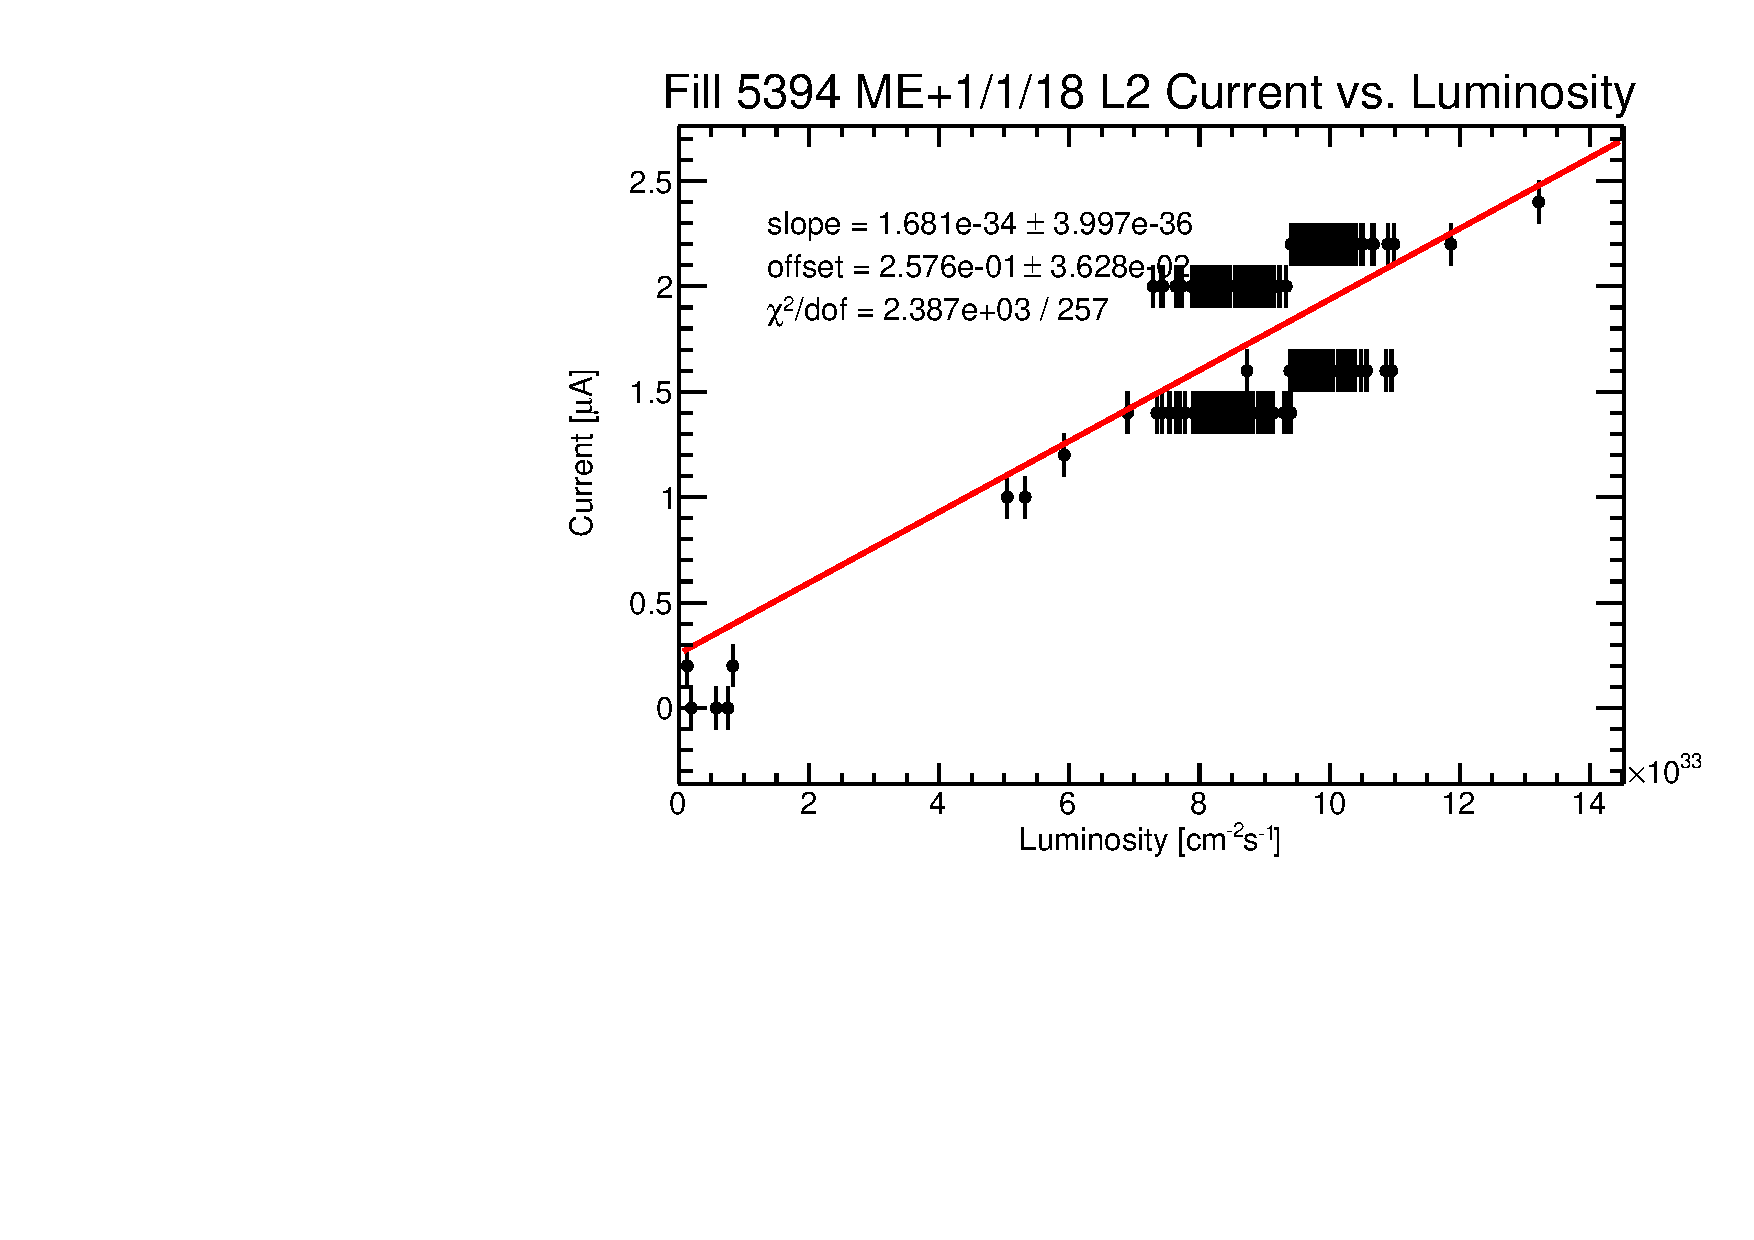
\includegraphics[width=0.7\twoThirdsFigWidth]{figures/neutron/ME11_P_18_2_f5394_curr_lumi.pdf}
  \caption[Plot of anode HV current \vs LHC luminosity with a two-parameter linear fit for three ME1/1 channels.]{Plot of anode HV current \vs LHC luminosity with a two-parameter linear fit for (\posstyle{top}) a well-behaved ME1/1 channel, (\posstyle{middle}) an ME1/1 channel with a large fitted offset, and (\posstyle{bottom}) a noisy ME1/1 channel.}
	\label{fig:ME11_IvsL}
\end{figure}

However, since the HVPSs for the ME1/1 chambers at CMS are known to measure a non-zero offset of HV current at zero luminosity, some adjustment of the HV current is necessary. In addition, in some ME1/1 HV channels, the HVPS can produce very noisy measurements of the anode HV current, resulting in data that are inconsistent with a straight line fit. \Fig~\ref{fig:ME11_IvsL} displays three plots of anode HV current \vs luminosity. The top plot is an example of a well-behaved ME1/1 channel that does not have an offset in the vertical intercept, so that we can use it to calculate the reference HV current. The middle plot is an example of ME1/1 channels that have a large offset of 0.46\muA that needs to be corrected when calculating the reference HV current. The bottom plot is an example of a noisy HV channel where the HVPS reads out hundreds of values of the HV current within a short period of time where the measured values oscillate between two values separated by 0.6\muA and is not consistent with the model of a straight line fit.

To avoid problems such as large offsets and many oscillating values, we scanned through all 432 ME1/1 HV channels in LHC fill 5394. We selected what we thought were the best channels, similar in appearance to the top plot in \FigDot~\ref{fig:ME11_IvsL}, based on fit $\chi^{2}$, number of degrees of freedom, and our own judgment. We applied this list of 157 (out of 432 possible) selected channels for use in all other LHC fills considered. We considered a total of 23 fills in this study. 

\begin{figure}
	\centering
	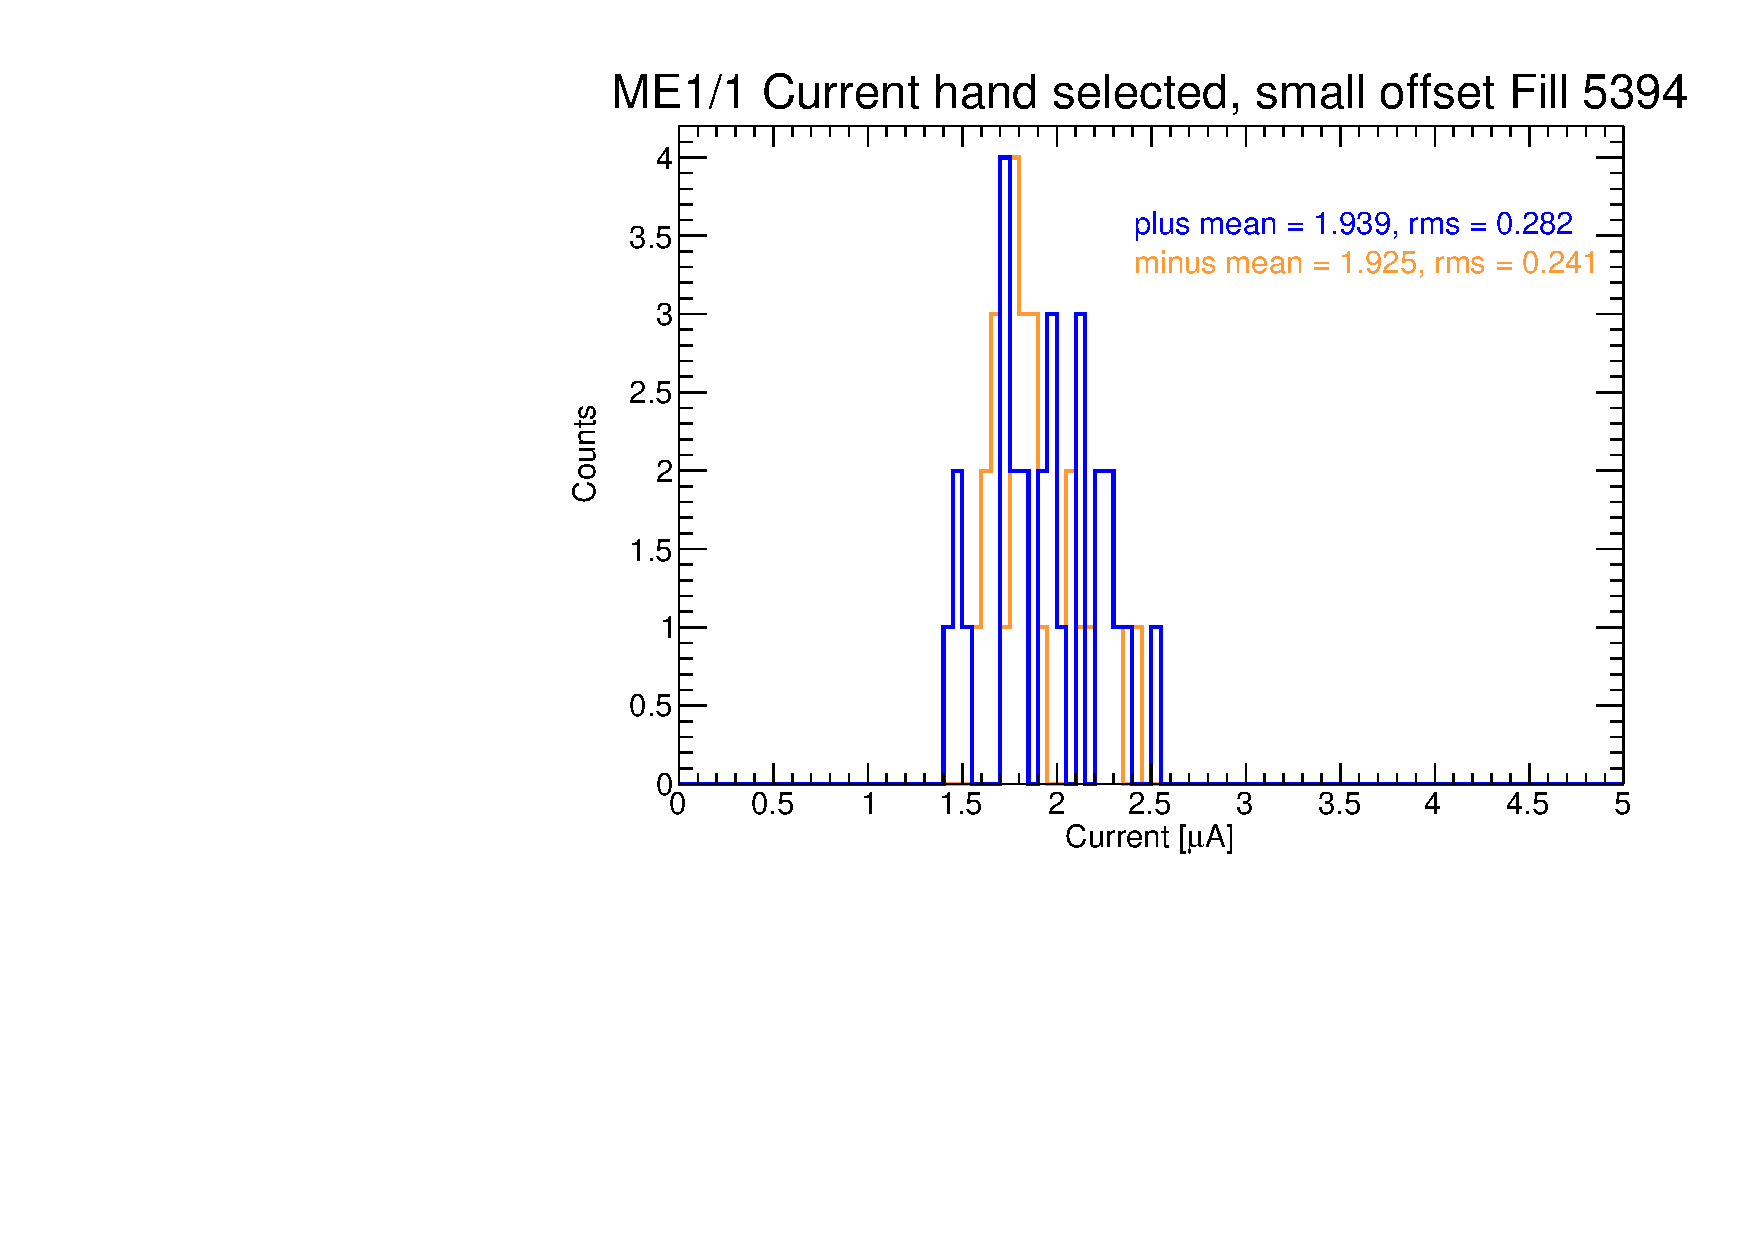
\includegraphics[width=\dummyFigWidth]{figures/neutron/me11_fill_5394_a_sel_slope_hist.pdf}
  \caption[Histogram of offset-corrected reference HV currents from ME1/1 HV channels.]{Histogram of offset-corrected reference HV currents from ME1/1 HV channels that pass the hand selection color-coded by endcap.}
	\label{fig:fill_5394_curr_histo}
\end{figure}

\Fig~\ref{fig:fill_5394_curr_histo} is a histogram of reference HV current values at the reference luminosity from hand-selected channels with the offset required to be less than $\pm$0.1\muA. To obtain one characteristic HV current value for each fill, we take the average of the plus and minus endcaps. Then to combine the measurements over all fills, we take the average of the HV currents in each fill during Run 2016H, with each fill weighted by its integrated luminosity. The averaged HV current is then multiplied by 6 because each CSC chamber has six HV channels (one per chamber layer) which operate independently. The resulting total ME1/1 chamber HV current is 

\begin{equation}
	I_{\text{ME1/1}} = 11.3\muA
\end{equation}

at the reference luminosity.

\begin{figure}
	\centering
	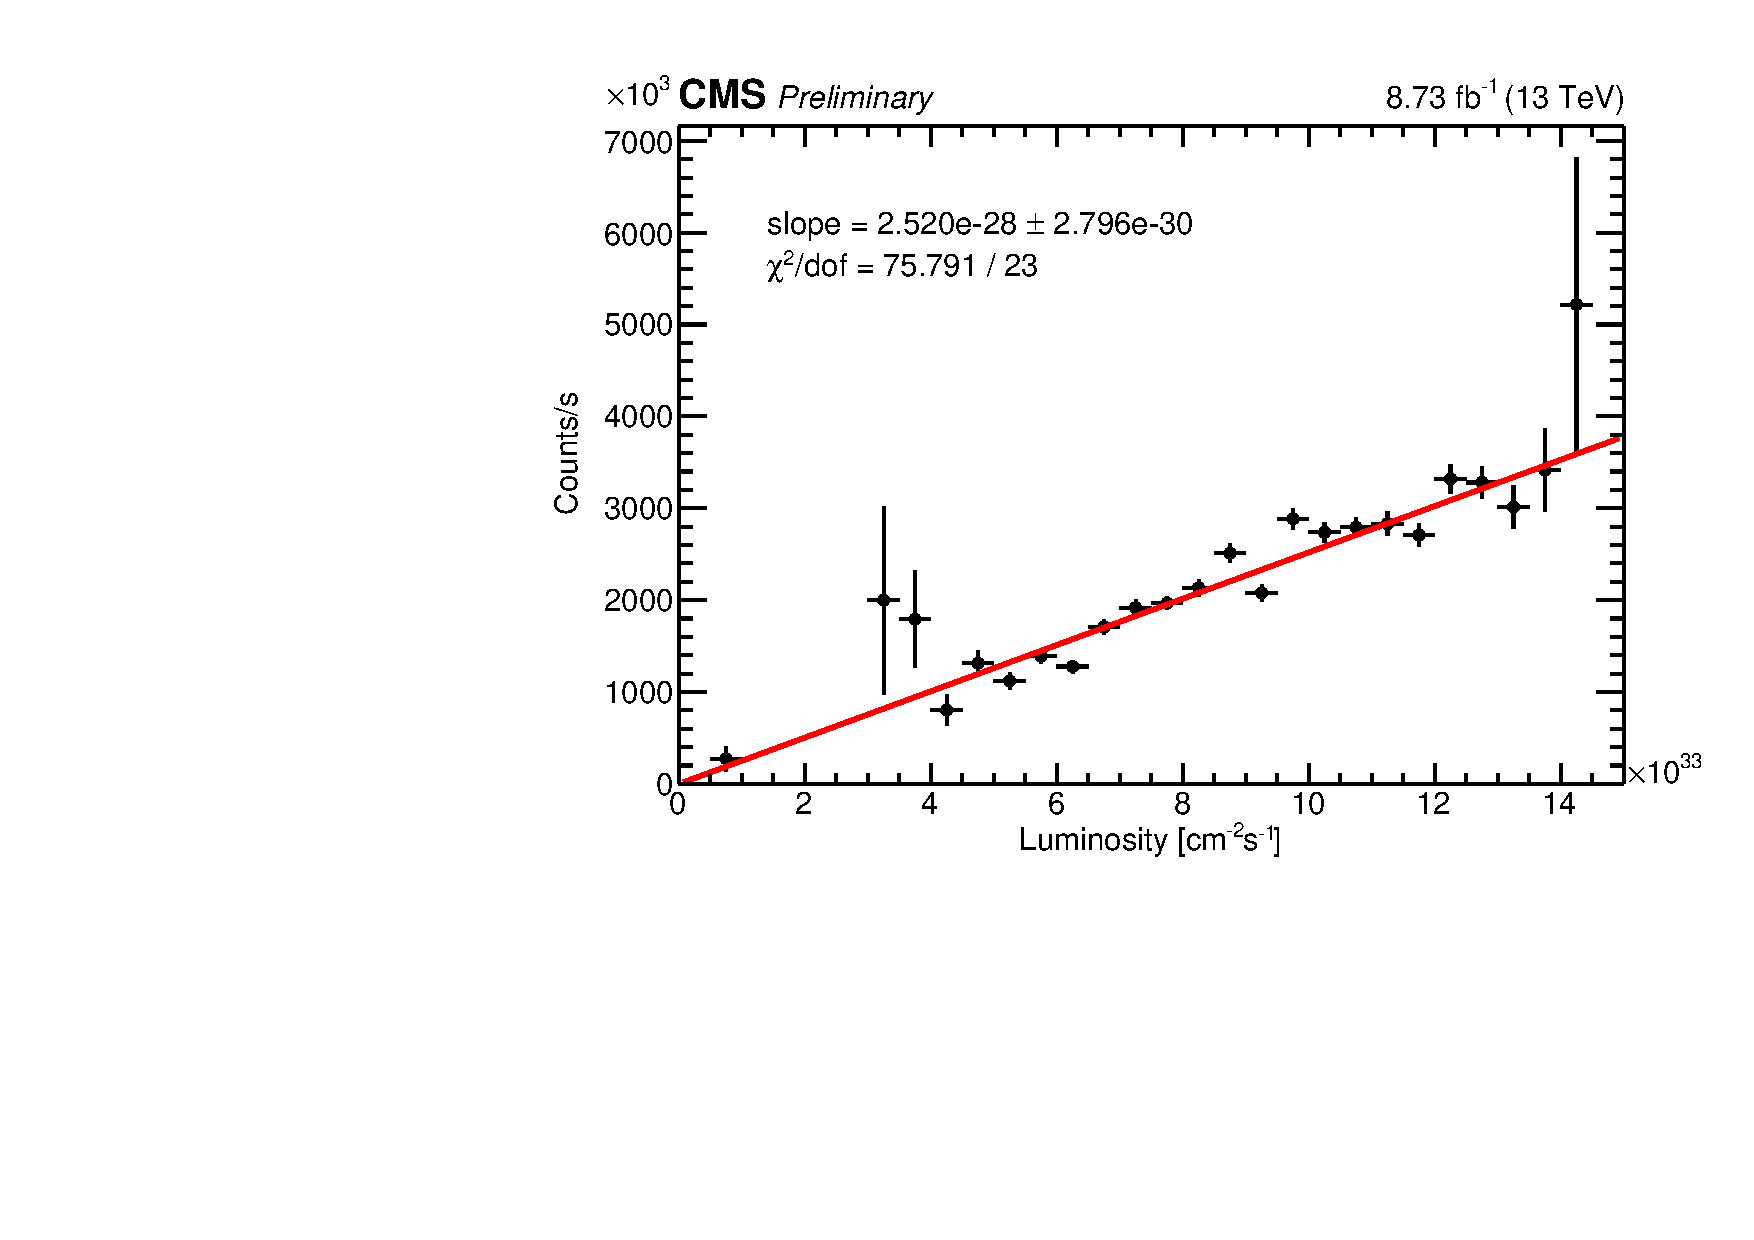
\includegraphics[width=\dummyFigWidth]{figures/neutron/luminosity_11_wire_early_CHAM_TIME_20180416_fit.pdf}
	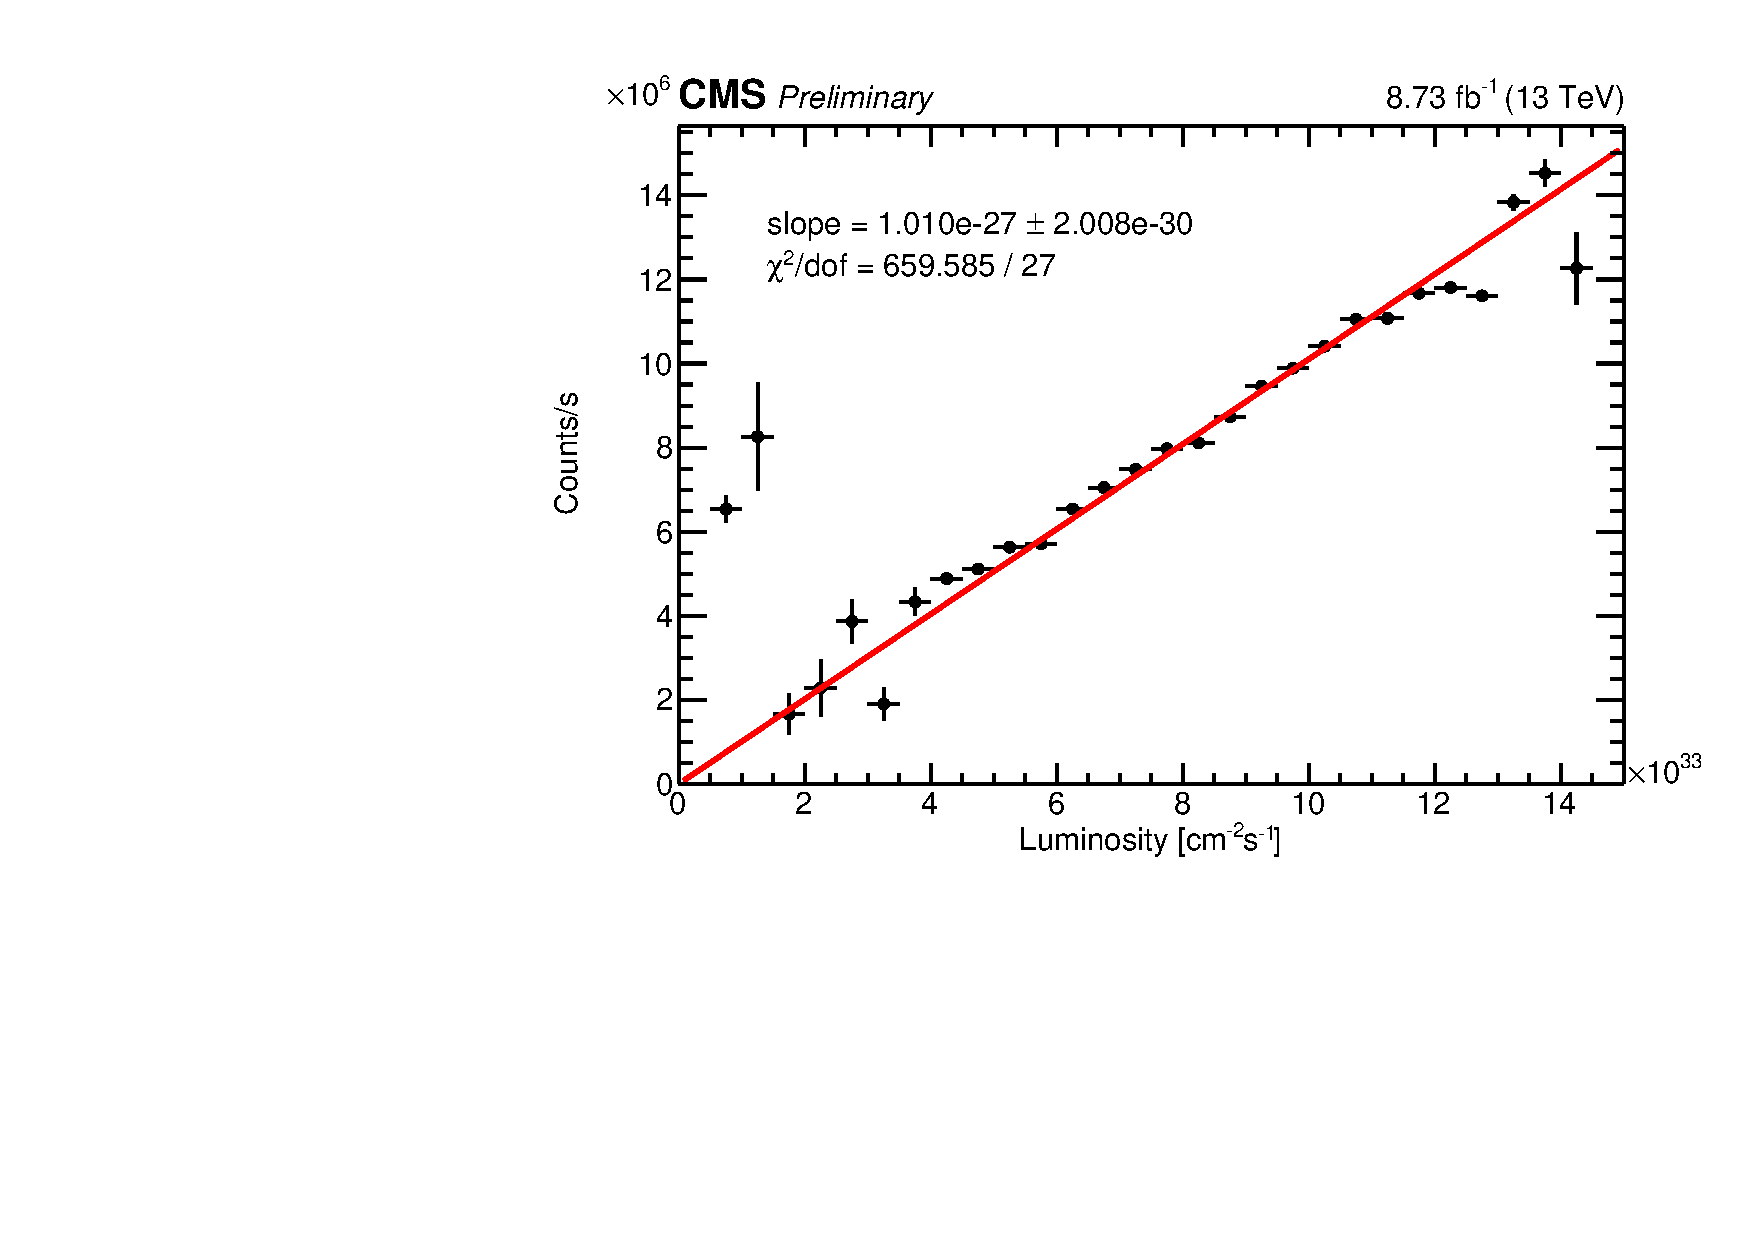
\includegraphics[width=\dummyFigWidth]{figures/neutron/luminosity_11_wire_total_CHAM_TIME_20180416_fit.pdf}
  \caption[Plot of ME1/1 wire group ${N}^\text{CMS}_\text{hits} / {t}$ \vs LHC luminosity with a one-parameter linear fit for hits that occur during LHC bunch gaps and during \pp collisions.]{Plot of ME1/1 wire group ${N}^\text{CMS}_\text{hits} / {t}$ \vs LHC luminosity with a one-parameter linear fit for hits that occur (\posstyle{top}) during LHC bunch gaps and (\posstyle{bottom}) during \pp collisions.}
	\label{fig:ME11_HvsL}
\end{figure}


To obtain the reference rate of anode wire group hits, we start by calculating the values of the\unit{hits/s} at the reference luminosity \reflumi from the slopes of one-parameter linear fit to plots of\unit{hits/s} \vs luminosity in \FigDot~\ref{fig:ME11_HvsL}. The top plot in \FigDot~\ref{fig:ME11_HvsL} is the ME1/1 wire group\unit{hits/s} \vs LHC luminosity (from \Eq~\ref{eqn:hits_perA_perT_perCSC} but without the $1 / A_\text{CSC}$ factor) for wire group hits that occur in LHC bunch gaps (lower left triangle from \FigDot~\ref{fig:rainbow}); the bottom plot is the same but for wire group hits that occur during \pp collisions (middle rectangle from \FigDot~\ref{fig:rainbow}). The reference rate of anode wire group\unit{hits/s} is sum of the hit rates of hits occurring in LHC gaps, $H_\text{LHC gap}$, and during LHC bunch trains, $H_\text{\pp-coll}$, weighted by the LHC bunch fill fraction, $f_\text{fill} = 0.62$,: 

\begin{equation}
	\begin{split}
	\label{eqn:hit_rate_calc}
	H_{\text{WG-ME1/1}} &= f_{\text{fill}} \  H_\text{\pp-coll} + (1-f_{\text{fill}}) \  H_{\text{LHC gap}} \\
	&= 0.62  \  10.1\times10^6 \unit{hits/s} + 0.32  \  2.5\times10^{5} \unit{hits/s} \\
	&= 7.2 \times 10^{6}\unit{hits/s}.
\end{split}
\end{equation}

The\unit{charge/hit} is then calculated by dividing the anode HV current by the anode wire group\unit{hits/s}:

\begin{equation}
	\label{eqn:ME11_chph_calc}
	\text{\text{charge}/\text{hit}} = I_{\text{ME1/1}}/H_{\text{WG-ME1/1}} = (11.3 \muA)/(7.2 \times 10^{6}\unit{hits/s}) = 1570\unit{fC/hit}.
\end{equation}



\subsubsection{ME2/1}
\begin{figure}
    \centering
    \includegraphics[width=0.7\twoThirdsFigWidth]{figures/neutron/ME21_P_04_1_5_f5394_curr_lumi.pdf}
    \includegraphics[width=0.7\twoThirdsFigWidth]{figures/neutron/ME21_P_04_2_5_f5394_curr_lumi.pdf}
    \includegraphics[width=0.7\twoThirdsFigWidth]{figures/neutron/ME21_P_04_3_5_f5394_curr_lumi.pdf}
    \caption[Plot of current \vs luminosity for ME+2/1/04 layer 5 for three HV Segments with a two-parameter linear fit.]{Plot of current \vs luminosity for ME+2/1/04 layer 5 for HV Segment (\posstyle{top}) 1, (\posstyle{middle}) 2, and (\posstyle{bottom}) 3, with a two-parameter linear fit. The least count of approximately 0.1\muA is most evident in HV segment 3.}
    \label{fig:ME21_curr_lumi_p214_5}
\end{figure}

ME2/1 chambers each have 18 independent HV channels. Each of a chamber's six layers is divided into three HV segments: one HV segment, through which passes the highest current, is close to the beam line; one HV segment, through which passes a lower current, is in the center of the chamber; and one HV segment, through which passes the lowest current, is at the end of the chamber furthest from the beam line. \Fig~\ref{fig:ME21_curr_lumi_p214_5} displays plots of the anode HV current \vs luminosity for a representative example of ME2/1 chambers, ME+2/1/04 Layer 5, for all three HV segments.

\begin{figure}
	\centering
	\includegraphics[width=\dummyFigWidth]{figures/neutron/luminosity_21_wire_early_CHAM_TIME_20180416_fit.pdf}
	\includegraphics[width=\dummyFigWidth]{figures/neutron/luminosity_21_wire_total_CHAM_TIME_20180416_fit.pdf}
  \caption[Plot of ME2/1 wire group ${N}^\text{CMS}_\text{hits}/{t}$ \vs LHC luminosity for hits that occur during LHC bunch gaps and during \pp collisions.]{Plot of ME2/1 wire group ${N}^\text{CMS}_\text{hits}/{t}$ \vs LHC luminosity for hits that occur (\posstyle{top}) during LHC bunch gaps and (\posstyle{bottom}) during \pp collisions, with a one-parameter linear fit.}
	\label{fig:ME21_HvsL}
\end{figure}

\begin{figure}
	\centering
	\includegraphics[width=\dummyFigWidth]{figures/neutron/occupancy_21_wire_total_CHAM_TIME_20180416.pdf}
  \caption[Plot of anode wire group ${N}^\text{CMS}_\text{hits}(d)/{t}$ that occur during \pp collisions in ME2/1.]{Plot of anode wire group ${N}^\text{CMS}_\text{hits}(d)/{t}$ that occur during \pp collisions in ME2/1. HV segment 1 is wire group numbers 1--45, HV segment 2 is wire group numbers 46--81, and HV segment 3 is wire group numbers 82--112.}
	\label{fig:ME21_inTrain_occ}
\end{figure}

We start by calculating the rate of wire group hits in ME2/1 for the full chamber in the same way as ME1/1. \Fig~\ref{fig:ME21_HvsL} displays plots of the rate of ME2/1 wire group hits second for hits occurring at the end of LHC bunch gaps and during \pp collisions with a one-parameter linear fit through the origin. The slopes are again used as the reference hit rate and are combined according to \Eq~\ref{eqn:hit_rate_calc}. This gives an estimate of the hit rate in\unit{hits/s} for ME2/1, denoted as $H_\text{WG-ME2/1}$.

We then count the number of hits that occur within each HV segment. This number divided by the total number of hits in the chamber is the fraction of hits $f_{\text{ME2/1-}s}$ that occur in each HV segment, where $s=$1, 2, or 3 for each HV segment. The boundaries of HV segments are visible in \FigDot~\ref{fig:ME21_inTrain_occ} as dips in the occupancy plot at wire groups 45 and 81. HV segment 1 is taken as wire group numbers 1--45, HV segment 2 as 46--81, and HV segment 3 as 82--112. \Tab~\ref{tab:21_hit_frac} reports the hit fractions calculated from \FigDot~\ref{fig:ME21_inTrain_occ}. The rate of wire group hits in each HV segment at the reference luminosity is then obtained by multiplying the hit fraction for each HV segment to the full ME2/1 rate of wire group hits, 

\begin{equation}
	\label{eqn:ME21_HR_calc}
	H_{\text{WG-ME2/1-}s}=f_{\text{ME2/1-}s}  \  H_{\text{WG-ME2/1}}.
\end{equation}

These hit rates are also reported in \Tab~\ref{tab:21_hit_frac}. 

\begin{table}
	\centering
	\topcaption{Values of wire group hit fraction and hit rate in each ME2/1 HV segment.}
	\label{tab:21_hit_frac}
	\begin{tabular}{c|cc}
				& $f_{\text{ME2/1-}s}$    & $H_{\text{WG-ME2/1-}s}$ [hits/s]\\ \hline
	ME2/1       & -                       & 6.3$\times10^{6}$       \\ \hline
	ME2/1 S1    & 0.63                    & 3.9$\times10^{6}$       \\ \hline
	ME2/1 S2    & 0.25                    & 1.5$\times10^{6}$       \\ \hline
	ME2/1 S3    & 0.12                    & 0.8$\times10^{6}$       \\ 
	\end{tabular}
\end{table}

The next step we take is to convert the luminosity values of all points in \FigDot~\ref{fig:ME21_curr_lumi_p214_5} to equivalent \unit{hits/s}. To do this, we multiply the luminosity value of each point, denoted $\pazocal{L}$, by the \unit{hits/s} at \reflumi, $H_{\text{WG-ME2/1-}s}$, in each HV segment.

\begin{equation}
	\label{eqn:lumi_to_hitrate}
	\text{hits/s} = \pazocal{L} \times H_{\text{WG-ME2/1-}s}
\end{equation}

\begin{figure}
	\centering
	\includegraphics[width=\twoThirdsFigWidth]{figures/neutron/ME21_P_04_5_f5394_curr_hitrate.pdf}
	\includegraphics[width=\twoThirdsFigWidth]{figures/neutron/ME21_P_04_6_f5394_curr_hitrate.pdf}
  \caption[Plot of HV current \vs\unit{hits/s} for an ME2/1 layer with smooth transitions in current and a jump in HV current.]{Plot of HV current \vs\unit{hits/s} for an ME2/1 layer (\posstyle{top}) with smooth transitions in current and\unit{hits/s} between HV segments and (\posstyle{bottom}) Plot of HV current \vs\unit{hits/s} for an ME2/1 layer with a jump in HV current and\unit{hits/s} between HV segments 1 and 2. Segment 1 is in blue, segment 2 is in green, and segment 3 is in red.}
	\label{fig:ME21_IvsH}
\end{figure}

This transformation from luminosity to equivalent \unit{hits/s} gives us the HV current as a function of\unit{hits/s} in each ME2/1 segment individually. \Fig~\ref{fig:ME21_IvsH} displays example HV current \vs \unit{hits/s} for ME+2/1/04 Layer~5 and Layer~6. 

At CMS, the non-ME1/1 chambers use a different HVPS system than the ME1/1 chambers. When the non-ME1/1 HVPS were commissioned in CMS, each HV channel in the non-ME1/1 chambers was independently calibrated from each other. As a check of this, we study plots of current \vs luminosity and we verify that it is not necessary to correct for fitted offsets when computing the fitted reference current values. However, we observe that for some non-ME1/1 chambers, there are layer-by-layer differences in current in a given chamber and given LHC fill at the same hit rate. \Fig~\ref{fig:ME21_IvsH} displays example HV current \vs \unit{hits/s} plots for ME+2/1/04 Layer~5 and Layer~6. The top plot (Layer~5) shows that when different HV segments in the same chamber have similar\unit{hits/s}, they do have similar HV currents. However, for some channels, a noticeable jump is observed in the HV current at similar\unit{hits/s}, as in the bottom plot (Layer~6). This discrepancy might be caused by some amount of miscalibration of the HVPS conversion of ADC to$\,$\muA. To avoid channels with possible miscalibration, we scan through plots of HV current \vs\unit{hits/s} for all layers of ME2/1 chambers and search for subjectively defined smooth transitions in HV current and\unit{hits/s} between each segment. 

\begin{figure}
	\centering
	\includegraphics[width=\dummyFigWidth]{figures/neutron/ME21_f5394_chph_sel_hist.pdf}
	\caption{Histogram of values of\unit{charge/hit} in fC in ME2/1 for LHC Fill 5394.}
	\label{fig:ME21_fill_5394_chph_histo}
\end{figure}

We then calculate\unit{charge/hit} by dividing the $y$ axis value (HV current) by the $x$ axis value (hits$/$s) of each data point in the HV current \vs\unit{hits/s} plots for all three HV segments in each selected chamber layer. Each\unit{charge/hit} value is collected into a histogram for each LHC fill during run period H of 2016. One entry in this histogram is a single data point from plots of HV current \vs\unit{hits/s} in chamber layers that pass our selection. \Fig~\ref{fig:ME21_fill_5394_chph_histo} is an example of the\unit{charge/hit} histogram of selected chamber layers for each HV segment for LHC Fill 5394. (Fill 5394 was used to determine the selection of good ME2/1 layers.) HV segment 1 is the blue histogram, HV segment 2 is the green histogram, and HV segment 3 is the red histogram. HV segment 3 is bi-modal because at very low HV current (less than approximately 0.6\muA) the HV current ADC least count of approximately 0.1\muA is the dominant source of uncertainty which causes measured values of the HV current to fluctuate between the two closest least count values.

To obtain a\unit{charge/hit} value in each fill and HV segment, we use the mean of each of the\unit{charge/hit} histogram. Then finally, just as the HV current measurements in ME1/1 were combined, the\unit{charge/hit} for each HV segment in each LHC fill is averaged with a weighting according to the integrated luminosity of each fill considered. For HV segment 3 this procedure gives a 4\% larger\unit{charge/hit} than by computing the ratio of the HV current averaged over fills and the\unit{hits/s} from \Tab~\ref{tab:21_hit_frac}.

\subsection{Computation of charge/hit from GIF++ data}
\begin{figure}
	\centering
	\includegraphics[width=\halfFigWidth]{figures/neutron/g_ALL_C1.pdf}\hspace*{-1em}
	\includegraphics[width=\halfFigWidth]{figures/neutron/g_S1_C110.pdf}
	\includegraphics[width=\halfFigWidth]{figures/neutron/g_S2_C110.pdf}\hspace*{-1em}
	\includegraphics[width=\halfFigWidth]{figures/neutron/g_S3_C110.pdf}
  \caption[Plot of anode HV current \vs\unit{hits/s} at GIF++ for ME1/1 and ME2/1 HV segments.]{Plot of anode HV current \vs\unit{hits/s} at GIF++ for (\posstyle{top left}) ME1/1 and ME2/1 HV segment (\posstyle{top right}) 1, (\posstyle{bottom left}) 2, and (\posstyle{bottom right}) 3.}
	\label{fig:GIF_IvsH}
\end{figure}

At GIF++, the\unit{charge/hit} for background hits is obtained by measuring the anode HV current and the rate of early time anode wire groups hits in externally triggered data at each source attenuation. \Fig~\ref{fig:GIF_IvsH} displays plots of the measured anode HV current as a function of the total number of anode wire group hits that occur in readout time bins 1--5 for the ME1/1 and ME2/1 chambers at GIF++ respectively. Each dot represents a single source attenuation, where the lowest source intensity yields the lowest HV current and lowest background\unit{hits/s}, and increasing the source intensity also increases the HV current and anode wire\unit{hits/s} roughly linearly. The slopes of the fitted lines represent the measured\unit{charge/hit} of each CSC. For ME2/1, only the first 8 points are used to calculate the slope, because at higher source intensities, the high HV currents passing through the internal resistance result in a non-negligible drop in the HV at the anode wire.

\subsection{Computation of charge/hit from CMS simulation}
\begin{figure}
	\centering
	\includegraphics[width=\dummyFigWidth]{figures/neutron/CPH_ME11.pdf}
	\includegraphics[width=\dummyFigWidth]{figures/neutron/CPH_ME21.pdf}
  \caption[Histogram of the avalanche charge per simulated wire hit for for ME1/1 and non-ME1/1 champers in CMS simulation.]{In simulation of CMS data, histogram of the avalanche charge per simulated wire hit for (\posstyle{top}) ME1/1 and (\posstyle{bottom}) non-ME1/1 chambers}
	\label{fig:cph_MC}
\end{figure}

In the HP neutron simulation as described above, each simulated wire hit can be associated to a quantity of simulated avalanche charge produced from the gas ionization. \Fig~\ref{fig:cph_MC} displays histograms of the simulated avalanche charges for ME1/1 and non-ME1/1 simulated wire hit. We take the mean of these histograms of total avalanche charge per simulated wire hit as a measure of\unit{charge/hit} in MC simulation for neutron-induced hits.

\subsection{Comparison of charge/hit}

\begin{table}
	\centering
  \topcaption[Values of\unit{charge/hit} in ME1/1 and each HV segment of ME2/1 in units of\unit{fC/hit}.]{Values of\unit{charge/hit} in ME1/1 and each HV segment of ME2/1 in units of\unit{fC/hit}. All non-ME1/1 chamber\unit{charge/hit} were observed to be similar. Therefore, the\unit{charge/hit} was measured by averaging all non-ME1/1 chambers; the * in the ME2/1 MC\unit{charge/hit} measurements indicates this.}
	\label{tab:charge_per_hit}
	\begin{tabular}{c|ccc}
	{[}fC/hit{]}                 & CMS                      & GIF++                    & MC                   \\ \hline
	ME1/1                        & 1570                     & 3780                     & 1360                 \\ \hline
	ME2/1 S1                     & 3451                     & 4010                     & 1420*                \\ \hline
	ME2/1 S2                     & 3274                     & 3720                     &                      \\ \hline
	ME2/1 S3                     & 3166                     & 3890                     &                      \\ 
	\end{tabular}
\end{table}

\Tab~\ref{tab:charge_per_hit} is the collection of all\unit{charge/hit} calculations in units of\unit{fC/hit} for ME1/1 and ME2/1 for CMS data, GIF++ data, and CMS simulation. 

To summarize the results: 
\begin{itemize}
	\item ME1/1\unit{charge/hit} at GIF++ is roughly a factor of 2.5 higher than at CMS
	\item ME1/1 MC\unit{charge/hit} matches ME1/1\unit{charge/hit} at CMS within 15\%
	\item ME2/1\unit{charge/hit} is a factor of 2--3 higher than ME1/1\unit{charge/hit} at CMS
	\item ME2/1\unit{charge/hit} at GIF++ is 20--30\% higher at GIF++ than at CMS
	\item ME2/1 MC\unit{charge/hit} is roughly 2--2.5 lower than ME2/1\unit{charge/hit} at CMS
\end{itemize}

These results are important for reconstruction studies, where the total\unit{hits/s} is the strongest indicator of trigger and software performance. This means that at equal\unit{hits/s} for CSCs at GIF++ and CMS (effects on muon reconstruction are roughly the same), the HV current will differ by the same amount as\unit{charge/hit}. So, when using HV current for correspondence between GIF++ source intensities and ME1/1, these results at face value imply that at an equal\unit{hits/s} the chamber at GIF++ will have a factor of 2.5 larger HV current than chambers in CMS. Similarly, for the ME2/1 chamber correspondence, the ME2/1 at GIF++ will have a 20--30\% larger HV current than the chambers in CMS assuming an equal\unit{hits/s} (depending on HV segment). However, further understanding of possible mis-calibration of HV current ADC to \muA conversion is necessary in the calculation of ME2/1\unit{charge/hit}. 

\section{Acknowledgments}
\label{sec:acknowledgments}

	We would like to thank everyone on the CSC GIF++ team, the CMS UCLA group, and everyone whose work we have built on or partially reproduced and who have contributed valuable knowledge and advice, including Cameron Bravo, Tim Cox, Alice Florent, Jay Hauser, Misha Ignatenko, Vladimir Ivantchenko, Evaldas Juska, Alexey Kamenev, Andrey Korytov, Katerina Kuznetsova, Armando Lanaro, Paul Lujan, Alex Madorsky, Nick McColl, Hualin Mei, Yuriy Pakhotin, Vladimir Palchik, Victor Perelygin, Jian Wang, Wells Wulsin, and Piet Verwilligen. This work was partially supported by the U.S.\ Department of Energy under Award Number {DE}--{SC}0009937.

Reference \cite{PietsPage} contains brief a history of the measurement of the neutron background in CMS with links to previous work done dating back to 1994.


\chapter{Conclusion}

%%%%%%%%%%%%%%%%%%%%%%%%%%%%%%%%%%%%%%%%%%%%%%%%%%%%%%%%%%%%%%%%%%%%%%

\bibliography{thesis}
\bibliographystyle {cmstdr_modified}

\end {document}

